%%%%%%%%%%%%%%%%%%%%%%%%%%%%%%%%%%%%%%%%%%%%%%%%%%%%%%%%%%%%%%%%%%%%%%%%%%%%%%%
% Author:  David Duarte
%
% Escuela de Ingeniería Electrónica
% Instituto Tecnológico de Costa Rica
%
% Tesis de Licenciatura
% 
% Phone:   +506 60348656
% email:   davidduarte28@gmail.com
%
%%%%%%%%%%%%%%%%%%%%%%%%%%%%%%%%%%%%%%%%%%%%%%%%%%%%%%%%%%%%%%%%%%%%%%%%%%%%%%%

% \documentclass is book
% If you want a printable two-side version of the thesis
%\documentclass[12pt,twoside,letterpaper]{book}

% If you want an electronic-only version of the thesis, do it one-sided
\documentclass[12pt,oneside,letterpaper]{book}

\usepackage[T1]{fontenc}
%\usepackage[utf8]{inputenc}   % is no longer required (since 2018)
\usepackage{ifthen}            % provide if-then-else operators
\usepackage{listings}
\usepackage{xcolor}

\definecolor{codegreen}{rgb}{0,0.6,0}
\definecolor{codegray}{rgb}{0.5,0.5,0.5}
\definecolor{codepurple}{rgb}{0.58,0,0.82}
\definecolor{backcolour}{rgb}{0.95,0.95,0.92}

\lstdefinestyle{mystyle}{
    backgroundcolor=\color{backcolour},   
    commentstyle=\color{codegreen},
    keywordstyle=\color{magenta},
    numberstyle=\tiny\color{codegray},
    stringstyle=\color{codepurple},
    basicstyle=\ttfamily\footnotesize,
    breakatwhitespace=false,         
    breaklines=true,                 
    captionpos=b,                    
    keepspaces=true,                 
    numbers=left,                    
    numbersep=5pt,                  
    showspaces=false,                
    showstringspaces=false,
    showtabs=false,                  
    tabsize=2
}

\lstset{style=mystyle}

% --------------------------------------------------------------------------
% Global variables required in document formatting
% --------------------------------------------------------------------------
%
% BOOK MODE
%
\newboolean{bookmode}                  % boolean used to control book format
% Ensure that only one of the next two lines is active:
\setboolean{bookmode}{true}           % turn book mode on
%\setboolean{bookmode}{false}           % turn book mode off

%
% DRAFT MODE
%   The draft mode activates the TODO index and some "draft" markings all
%   around.  Ensure you set it to false for the final version!!
%   
%
\newboolean{draftmode}                  % boolean used to control draft-mode

%% -------------------------------------------------------------------------

%% Configure su nombre, título de tesis, lectores, fechas, etc. en:
%%
%% >>>>  config.tex  <<<<
%%

% --------------------------------------------------------------------------

% include all packages and define all required general macros
%%%%%%%%%%%%%%%%%%%%%%%%%%%%%%%%%%%%%%%%%%%%%%%%%%%%%%%%%%%%%%%%%%%%%%%%%%%%%%%
% Author:  Pablo Alvarado
%
% Escuela de Electrónica
% Instituto Tecnológico de Costa Rica
%
% Phone:   +506 2550 9005
% email:   palvarado@itcr.ac.cr
% 
%%%%%%%%%%%%%%%%%%%%%%%%%%%%%%%%%%%%%%%%%%%%%%%%%%%%%%%%%%%%%%%%%%%%%%%%%%%%%%%

\PassOptionsToPackage{usenames,dvipsnames}{xcolor}

% -----------------------------------------------------------------------------
%   Define all configuration commands
% -----------------------------------------------------------------------------

\newcommand{\genderLector}[1]{%
  \ifthenelse{\equal{#1}{F}}{%
    Profesora Lectora%
  }{%
    \ifthenelse{\equal{#1}{M}}{%
      Profesor Lector%
    }{%
      Persona profesora lectora%
    }%
  }%
}

% Lector I
\newcommand{\nameLectorI}{$<$\emph{Use defLectorI in config.tex}$>$}
\newcommand{\genderLectorI}{N/A}

\newcommand{\defLectorI}[1][M]{%
  \renewcommand{\genderLectorI}{\genderLector{#1}}%
  \lectorIRelay%
}

\newcommand{\lectorIRelay}[1]{%
  \renewcommand{\nameLectorI}{#1}
}

%% Lector II
\newcommand{\nameLectorII}{$<$\emph{Use setLectorII in main.tex}$>$}
\newcommand{\genderLectorII}{N/A}

\newcommand{\defLectorII}[1][M]{%
  \renewcommand{\genderLectorII}{\genderLector{#1}}%
  \lectorIIRelay%
}

\newcommand{\lectorIIRelay}[1]{%
  \renewcommand{\nameLectorII}{#1}
}

%% Asesor
\newcommand{\nameAsesor}{$<$\emph{Use setAsesor in main.tex}$>$}
\newcommand{\genderAsesor}{$<$\emph{Use setAsesor in main.tex}$>$}

\newcommand{\defAsesor}[1][M]{%
  \ifthenelse{\equal{#1}{F}}{%
    \renewcommand{\genderAsesor}{Profesora Asesora}%
  }{%
    \ifthenelse{\equal{#1}{M}}{%
      \renewcommand{\genderAsesor}{Profesor Asesor}%
    }{%
      % La RAE no ha definido cómo hacer esto...
      %
      % Hay que preguntar a la persona asesora no-binaria directamente
      % cómo gusta ser tratada.
      \renewcommand{\genderAsesor}{Persona profesora asesora}%
    }
  }
  \asesorRelay
}

\newcommand{\asesorRelay}[1]{%
  \renewcommand{\nameAsesor}{#1}
}

% Dates for draft and final
\newcommand{\thesisDraftDate}{\today}
\newcommand{\defDraftDate}[1]{\renewcommand{\thesisDraftDate}{#1}}

\newcommand{\thesisFinalDate}{$<$\emph{Fecha de Defensa en config.tex}$>$}
\newcommand{\defFinalDate}[1]{\renewcommand{\thesisFinalDate}{#1}}

% Author definition and gender related strings

\newcommand{\thesisAuthor}{Error: Undefined}
\newcommand{\thesisAuthorShort}{Error: Undefined}
\newcommand{\thesisAuthorTECID}{Error: Undefined}
\newcommand{\thesisAuthorAddress}{Error: Undefined}
\newcommand{\thesisAuthorDegree}{Error: Undefined}

\newcommand{\defAuthor}[1][M]{%
  \ifthenelse{\equal{#1}{F}}{%
    \renewcommand{\thesisAuthorAddress}{la señora}
    \renewcommand{\thesisAuthorDegree}{Ingeniera}
  }{%
    \ifthenelse{\equal{#1}{f}}{%
      \renewcommand{\thesisAuthorAddress}{la señorita}
      \renewcommand{\thesisAuthorDegree}{Ingeniera}
    }{%
      \ifthenelse{\equal{#1}{M}}{%
        \renewcommand{\thesisAuthorAddress}{el señor}
        \renewcommand{\thesisAuthorDegree}{Ingeniero}
        
      }{%
        \renewcommand{\thesisAuthorAddress}{la persona}
        \renewcommand{\thesisAuthorDegree}{Ingeniere}
      }
    }
  }
  \authorRelay
}

\newcommand{\authorRelay}[1]{%
  \renewcommand{\thesisAuthor}{#1}
}

\newcommand{\defAuthorShort}[1]{%
  \renewcommand{\thesisAuthorShort}{#1}
}

\newcommand{\defAuthorTECID}[1]{%
  \renewcommand{\thesisAuthorTECID}{#1}
}

%% About the institution and department
\newcommand{\thesisDepartment}{Escuela de Ingeniería Electrónica}
\newcommand{\thesisInstitution}{Tecnológico de Costa Rica}

\newcommand{\defDepartment}[1]{%
  \renewcommand{\thesisDepartment}{#1}
}

\newcommand{\defInstitution}[1]{%
  \renewcommand{\thesisInstitution}{#1}
}



%% About the report name, and type
\newcommand{\thesisTitle}{Error: Undefined}
\newcommand{\thesisFlatTitle}{\thesisTitle}
\newcommand{\thesisKeywords}{Error: Undefined}
\newcommand{\thesisType}{Error: Undefined}

%% A tool to remove new lines leaving no spaces
\newcommand\titleFlattener[1]{\def\\{\relax\ifhmode\unskip\fi\space\ignorespaces}#1}

\newcommand{\defTitle}[1]{%
  \renewcommand{\thesisFlatTitle}{\titleFlattener{#1}}
  \renewcommand{\thesisTitle}{#1}
}

\newcommand{\defKeywords}[1]{%
  \renewcommand{\thesisKeywords}{#1}
}

\newcommand{\defTFGType}[1]{%
  \renewcommand{\thesisType}{#1}
}

%% Este archivo contiene toda la configuración básica del documento de
%% tesis, para centralizar alguna información que se requiere en todo
%% el documento.

%% DRAFT MODE

%%   El modo borrador activa las listas de cosas por hacer, con su
%%   índice, y algunas marcas explícitas de "borrador" por todo lado.
%%
%%   Asegúrse de que esta variable sea false en la versión final y de haber
%%   actualizado la fecha de la defensa, un poco más abajo.
\setboolean{draftmode}{true}            % turn draft mode on
%\setboolean{draftmode}{false}          % turn draft mode off

%% Esta es la fecha que se colocará en el modo borrador
\defDraftDate{\today}
%% Esta es la fecha que se usará en la versión final
\defFinalDate{24 de noviembre, 2024}

%% Este es el nombre del estudiante y el pronombre que utiliza, para cambiar
%% las portadas como corresponde

% Con el nombre de autor, se debe especificar el género a utilizar:
%
%   [M]asculino
%   [F]emenino (usando "señora" donde corresponda)
%   [f]emenino (usando "señorita" donde corresponda)
%   persona [N]o binaria
%
%   Debido a la falta de norma en español para las personas no binarias,
%   posíblemente deba ajustarse para el gusto de cada quien.
%
\defAuthor[M]{David Duarte Sánchez}                % Nombre del estudiante
%\defAuthor[f]{María del Pilar Pérez Prado}    % Nombre de la estudiante

\defAuthorShort{D.~Duarte}                      % Nombre corto
\defAuthorTECID{2017239606}                     % Carné

%% Este es el título completo del informe del trabajo final de graduación.
%% Usted puede agregar \\ para forzar líneas nuevas en la portada y automática-
%% mente el comando se encarga de eliminar eso cuando necesita el título
\defTitle{Desarrollo de un conjunto de flujos de trabajo \\
          para la implementación de software a bordo de \\
          computadoras de guía, navegación y control espacial}

%% Palabras clave
\defKeywords{GNC, Sistemas, procesadores embebidos, marcos de trabajo, model to model transofrmation, codigo embebido}

%% Tribunal Evaluador
%%
%% Indique los nombres de los lectores y asesor
%% El parámetro opcional es
%%  [M]asculino,
%%  [F]emenino,
%%  persona [N]o binaria
\defLectorI[M]{Dr.\,Alfonso Chaves Jiménez}
\defLectorII[M]{Ing.\,William Marín Moreno}
\defAsesor[M]{Dr.\,Johan Carvajal Godínez}

%% Tipo de tesis o informe
%%   - Tesis de Licenciatura
%%   - Informe de Proyecto Final 
%%   - Tesis de Maestría
\defTFGType{Tesis de Licenciatura}

%% Nombre del departamento e institución
\defInstitution{Instituto Tecnológico de Costa Rica}
\defDepartment{Escuela de Ingeniería Electrónica}

 % Load the desired configuration

%Para el PDF (cambiar si se desea otras cosas a lo indicado arriba
\newcommand{\pdfAuthor}{\thesisAuthor}
\newcommand{\pdfTitle}{\thesisFlatTitle} 
\newcommand{\pdfKeywords}{\thesisKeywords}
\newcommand{\pdfSubject}{\thesisType}


%% -------------------------------------------------------------------

\usepackage{ifpdf}

% Command to change between draft or release mode:
\newcommand{\ifdraft}[2]{\ifthenelse{\boolean{draftmode}}{#1}{#2}}
% Command to change between draft or release mode:
\newcommand{\ifbook}[2]{\ifthenelse{\boolean{bookmode}}{#1}{#2}}

% include all required packages here
\usepackage{csquotes}                  % recommended for biblatex
\usepackage[spanish,es-tabla]{babel}   % spanish, remove es-tabla for cuadro
%\usepackage[spanish]{babel}   % spanish, remove es-tabla for cuadro

\usepackage{xspace} % Decide if a space is needed at the end of some commands

\makeatletter
% babel uses a hook and therefore the tablename is here not defined yet.
% However, it defines es@tablename with upper/lowercase, and we use it.
\ifthenelse{\equal{\es@tablename}{Ttabla}}{%
  \newcommand{\cuadro}{tabla}
  \newcommand{\cuadros}{tablas}
  \newcommand{\Cuadro}{Tabla}
  \newcommand{\elcuadro}{la tabla}
  \newcommand{\Elcuadro}{La tabla}
  \newcommand{\loscuadros}{las tablas}
  \newcommand{\Loscuadros}{Las tablas}
  
  \newcommand{\tabla}{tabla}
  \newcommand{\tablas}{tablas}
  \newcommand{\Tabla}{Tabla}
  \newcommand{\latabla}{la tabla}
  \newcommand{\Latabla}{La tabla}
  \newcommand{\lastablas}{las tablas}
  \newcommand{\Lastablas}{Las tablas}
  
  \newcommand{\tabref}[1]{\hyperref[#1]{tabla~\ref*{#1}}\xspace}
  \newcommand{\Tabref}[1]{\hyperref[#1]{Tabla~\ref*{#1}}\xspace}

  \newcommand{\latabref}[1]{la \tabref{#1}}
  \newcommand{\Latabref}[1]{La \tabref{#1}}

}{%
  \newcommand{\cuadro}{cuadro}
  \newcommand{\cuadros}{cuadros}
  \newcommand{\Cuadro}{Cuadro}
  \newcommand{\elcuadro}{el cuadro}
  \newcommand{\Elcuadro}{El cuadro}
  \newcommand{\loscuadros}{los cuadros}
  \newcommand{\Loscuadros}{Los cuadros}
  
  \newcommand{\tabla}{cuadro}
  \newcommand{\tablas}{cuadros}
  \newcommand{\Tabla}{Cuadro}
  \newcommand{\latabla}{el cuadro}
  \newcommand{\Latabla}{El cuadro}
  \newcommand{\lastablas}{los cuadros}
  \newcommand{\Lastablas}{Los cuadros}
  
  \newcommand{\tabref}[1]{\hyperref[#1]{cuadro~\ref*{#1}}\xspace}
  \newcommand{\Tabref}[1]{\hyperref[#1]{Cuadro~\ref*{#1}}\xspace}

  \newcommand{\latabref}[1]{el \tabref{#1}}
  \newcommand{\Latabref}[1]{El \tabref{#1}}

}
\makeatother

% References to figures
\newcommand{\figref}[1]{\hyperref[#1]{figura~\ref*{#1}}\xspace}
\newcommand{\Figref}[1]{\hyperref[#1]{Figura~\ref*{#1}}\xspace}
\newcommand{\lafigref}[1]{la \hyperref[#1]{figura~\ref*{#1}}\xspace}
\newcommand{\Lafigref}[1]{La \hyperref[#1]{figura~\ref*{#1}}\xspace}

% References to equations
\newcommand{\equ}[1]{\hyperref[#1]{(\ref*{#1})}\xspace}

% Refrences to chapters and sections
\newcommand{\capref}[1]{\hyperref[#1]{capítulo~\ref{#1}}\xspace}
\newcommand{\secref}[1]{\hyperref[#1]{sección~\ref{#1}}\xspace}

\usepackage{makeidx}                    % to create index file

\usepackage[nottoc]{tocbibind}          % Fix the hyperrefs to TOC,TOF, etc.
                                        % and ensure that they appear all in 
                                        % the Table of Contents
\ifdraft{%
  %\usepackage[refpage]{nomencl}        % Use to easily administrate the list
  \usepackage[intoc,spanish]{nomencl}   % of symbols
}{%
  \usepackage[intoc,spanish]{nomencl}
}

\usepackage{siunitx}                    % Units of the SI
\sisetup{output-decimal-marker = {,}}   % Use decimal , instead of decimal .
\DeclareSIQualifier\peak{p}
\DeclareSIQualifier\ppeak{pp}

\usepackage{amsmath}
\usepackage{amssymb,amstext}            % AMS-math and symbols package
\usepackage{mathrsfs}                   % Calygraphic fonts for transforms
\usepackage{trsym}                      % Para símbolos de transformadas o---o
\usepackage{stmaryrd}                   % For short arrows
\usepackage{nicefrac}
\usepackage{array}                      % extensions to tabular environment
\usepackage{longtable}                  % supports extraordinary long tables
\usepackage{tabularx}                   % supports tables with fixed width

\usepackage[backend=biber,              % Use biber/biblatex
            style=ieee,
            sorting=none,
            citestyle=numeric-comp]{biblatex}

\usepackage{afterpage}                  % put something only after the page
\usepackage{multirow}                   % supports multiple row grouping in 
                                        % tables
\usepackage{multicol}                   % multiple columns environments
\usepackage{enumitem}                   % better enumeration with paralist 
                                        % equivalents as follows:

\newlist{compactitem}{itemize}{3}
\setlist[compactitem]{topsep=0pt,partopsep=0pt,itemsep=0pt,parsep=0pt}
\setlist[compactitem,1]{label=\textbullet}
\setlist[compactitem,2]{label=---}
\setlist[compactitem,3]{label=*}

\newlist{compactdesc}{description}{3}
\setlist[compactdesc]{topsep=0pt,partopsep=0pt,itemsep=0pt,parsep=0pt}

\newlist{compactenum}{enumerate}{3}
\setlist[compactenum]{label*=\arabic*.,topsep=0pt,partopsep=0pt,itemsep=0pt,parsep=0pt}
\newlist{compactenuma}{enumerate}{3}
\setlist[compactenuma]{label*=\alph*.,topsep=0pt,partopsep=0pt,itemsep=0pt,parsep=0pt}

\usepackage{icomma}                     % decimal comma in math mode

\usepackage{bold-extra}

\usepackage[format=hang,%
            font=small,%
            labelfont=bf]{caption}      % nicer figure captions
\usepackage{subcaption}                 % for subfigures
            
\usepackage{booktabs}                   % book type tabulars
\usepackage{pdfpages}                   % used to include the final "acta"

% the own style with options depending on the draft mode
\ifdraft{%
\usepackage[todo]{sty/tecStyle}         % some command definitions
                                        % options [todo] todo-index
}{%
\usepackage{sty/tecStyle}               % some command definitions
                                        % options [todo] todo-index
}

%% fix the title for examples
\renewcommand{\examplelistname}{Índice de ejemplos}
\renewcommand{\examplename}{Ejemplo}

%% define some command to cope with the tribunal names

%% Lector I


\usepackage{url}                        % allows linebreaks at certain
                                        % characters or combinations of 
                                        % characters for URLs

%% Usual tikz libraries and configuration
\usepackage{tikz}
\usepackage{pgfplots}
\pgfplotsset{compat=1.16}
\usepgfplotslibrary{fillbetween}
\usetikzlibrary{patterns,shapes,arrows.meta,positioning,calc,babel}
\usetikzlibrary{fit,shapes.geometric,decorations.markings}

\usepackage{listings}                   % syntax highlighting of code fragments

\lstdefinestyle{verilog-style}
{
  language=Verilog,
  basicstyle=\small\ttfamily,
  keywordstyle=\color{dkblue},
  identifierstyle=\color{black},
  commentstyle=\color{dkgreen},
  numbers=left,
  numberstyle=\tiny\color{black},
  numbersep=10pt,
  tabsize=8,
  moredelim=*[s][\colorIndex]{[}{]},
  literate=*{:}{:}1
}
\lstset{literate=%
  {á}{{\'a}}1
  {é}{{\'e}}1
  {í}{{\'i}}1
  {ó}{{\'o}}1
  {ú}{{\'u}}1
  {ñ}{{\~n}}1
  {Á}{{\'A}}1
  {É}{{\'E}}1
  {Í}{{\'I}}1
  {Ó}{{\'O}}1
  {Ú}{{\'U}}1
  {Ñ}{{\~N}}1
}

\definecolor{vorange}{RGB}{255,143,102}

\makeatletter
\newcommand*\@lbracket{[}
\newcommand*\@rbracket{]}
\newcommand*\@colon{:}
\newcommand*\colorIndex{%
    \edef\@temp{\the\lst@token}%
    \ifx\@temp\@lbracket \color{black}%
    \else\ifx\@temp\@rbracket \color{black}%
    \else\ifx\@temp\@colon \color{black}%
    \else \color{vorange}%
    \fi\fi\fi
}
\makeatother


% For pdflatex
% - The hyperref package should always be loaded last, since it has to
%   overwrite some of the commands.
% - The package subfigure caused that the pagebackrefs and index refs were set
%   incorrectly.

\ifpdf
%
% final / draft document options
%\usepackage{graphicx}                   % for inserting pdf-graphics.
                                        % options final / draft
\ifdraft{%
\usepackage[%pdftex,%
            naturalnames=true,
            linktocpage,
            hyperindex,
            colorlinks,
            urlcolor=dkred,          %\href to external url
            filecolor=dkmagenta,     %\href to local file
            linkcolor=dkred,         %\ref and \pageref
            citecolor=dkgreen,       %\cite
            plainpages=false,
            pdfpagelabels,
            pdfpagemode=UseOutlines, % means use bookmarks (None,UseOutlines)
            % bookmarksopen=false,   % would show the whole hierarchy if true
            bookmarksnumbered=true,
            pdfpagelayout=OneColumn, % SinglePage,OneColumn,TwoColumnLeft,...
            pdfview=FitH, % FitB,FitBH,FitBV,Fit,FitH,FitV
            pdfstartview=FitH, % FitB,FitBH,FitBV,Fit,FitH,FitV
            unicode,
            ]{hyperref}
}{%
% Use biber/biblatex
\usepackage[%pdftex,%
            naturalnames=true,
            linktocpage,hyperindex,
            colorlinks,
            urlcolor=dkred,          %\href to external url
            filecolor=dkmagenta,     %\href to local file
            linkcolor=dkred,         %\ref and \pageref
            citecolor=dkgreen,       %\cite
            plainpages=false,
            pdfpagelabels,
            pdfpagemode=UseOutlines, % means use bookmarks (None,UseOutlines)
            % bookmarksopen=false,   % open the whole hierarchy if true!
            bookmarksnumbered=true,
            pdfpagelayout=OneColumn, % SinglePage,OneColumn,TwoColumnLeft,...
            pdfview=FitH, % FitB,FitBH,FitBV,Fit,FitH,FitV
            pdfstartview=FitH, % FitB,FitBH,FitBV,Fit,FitH,FitV,
            unicode,
            ]{hyperref}
}


%
% Ensure that the links of the images point to the top of the images and not
% to the caption
%
\usepackage[figure]{hypcap}

% %
% % Ensure that pdfLaTeX do the same spacing as LaTeX
% %
\pdfadjustspacing=1 
% %
\else   % i.e. if not pdf

\usepackage[active]{srcltx}             % insert links into the dvi to jump
\usepackage{graphicx}                   % for inserting eps-graphics.
                                        % options final / draft
                                        % into the sources directly.
\ifdraft{%
\usepackage[ps2pdf,%
            % plainpages=false,
            linktocpage,
            hyperindex,
            % pdfpagelabels,
            pdfpagemode=UseOutlines,
            pdfstartview=FitH,
            unicode,]{hyperref}
}{%
\usepackage[ps2pdf,%
            % plainpages=false,
            linktocpage,
            hyperindex,
            % pdfpagelabels,
            pdfpagemode=UseOutlines,
            pdfstartview=FitH,
            unicode,]{hyperref}
}

%\usepackage[ps2pdf]{hyperref}

\fi  % end of if pdf or not

% --------------------------------------------------------------------------

% Allow the use of international characters
\AtBeginDocument{%
  \hypersetup{%
             pdftitle={\pdfTitle},%
             pdfsubject={\pdfSubject},%
             pdfauthor={\pdfAuthor},%
             pdfkeywords={\pdfKeywords}
            }%
}


%\usepackage{algorithmic}            % algorithmic environment


\usepackage{rotating}                % allow block rotation

%% This environment will allow to rotate a page in the PDF, just
%% for visualization purposes.  Since nowadays the documents are
%% almost never printed, it is best if rotated pages are also shown
%% rotated in the PDF viewer, and this is the purpose of this environment.
\newenvironment{rotatepage}%
{\global\pdfpageattr\expandafter{\the\pdfpageattr/Rotate 90}}%
{\clearpage\pagebreak[4]\global\pdfpageattr\expandafter{\the\pdfpageattr/Rotate 0}}

    
%%%%%%%%%%%%%%%%%%%%%%%%%%%%%%%%%%%%%%%%%%%%%%%%%%%%%%%%%%%%%%%%%%%%%%%%%%%%%%%

%\sloppy

%
% Some own font definitions
%
\DeclareMathAlphabet{\mathpzc}{OT1}{pzc}{m}{it}
\DeclareMathAlphabet{\mathpss}{OT1}{cmss}{m}{sl}

%
% page layout
%

\usepackage{vmargin}
\setpapersize{USletter}

% For letter-paper printing
\setmarginsrb{33mm}{8mm}{23mm}{7mm}{15pt}{15pt}{7mm}{12mm}
%\setlength{\headheight}{15pt}         % fancy headers wanted this

%
% Fraction of Float Object / Text
%

\renewcommand{\topfraction}{0.95}       % how much of top of page should be 
                                        % allowed to be float object?
\renewcommand{\bottomfraction}{0.95}    % how much of bottom of page should be
                                        % allowed to be float object?
\renewcommand{\textfraction}{0.05}      % how much of page must be text?

\usepackage{fancyhdr}                   % fancy page headers

\usepackage{lastpage}

%
% header and footer layout (needs package fancyhdr)
%
\newcommand{\copyrightfooter}{\tiny{\copyright \the\year\ --- \thesisAuthorShort %
    \qquad Uso exclusivo ITCR}}
%
\newcommand{\draftfoot}%
  {\ifdraft{\textcolor{dkblue}{\tiny\textsl{Borrador: \today}}{}}
           {}
}

\pagestyle{fancy}
\renewcommand{\chaptermark}[1]{\markboth{{\small
    \thechapter\hspace*{1mm}#1}}{}}
\renewcommand{\sectionmark}[1]{\markright{{\small
    \thesection\hspace*{1mm}#1}}{}}
%\lhead[{\small\textsc\Roman{\thepage}}]{\fancyplain{}%
\lhead[{\small\thepage}]{\fancyplain{}%
        {{\slshape \small\nouppercase{\leftmark}}}}
\chead[]{}
\rhead[\fancyplain{}%
%        {{\slshape \small\nouppercase{\rightmark}}}]{{\small\textsc\Roman{\thepage}}}
        {{\slshape \small\nouppercase{\rightmark}}}]{{\small\thepage}}
\lfoot[]{\draftfoot}
\ifbook{%
  \cfoot[]{}
}{
  \cfoot[\copyrightfooter]{\copyrightfooter}
}
\rfoot[\draftfoot]{}
\renewcommand{\headrulewidth}{0.5pt}
\renewcommand{\footrulewidth}{0pt}

%
% Caption style for tables
% For caption v3:
\captionsetup[table]{position=top,
  format=hang,
  textfont={normalsize},
  labelfont={normalsize,bf}}

\newcommand{\tablecaption}[2][foo]{%
  \ifthenelse{\equal{#1}{foo}}{%
    \caption{#2}%
  }{%
    \caption[#1]{#2}%
  }
}

%% En español hay diferencia entre Tabla y Cuadro.
%%
%% Tabla: es la tabla periódica, o una tabla de logaritmos o de
%%        probabilidades o de integrales. Usualmente es algo que no
%%        requiere referencias o explicaciones adicionales en el texto porque
%%        todas sus entradas son sucesiones de alguna cosa que se busca allí
%%        mismo
%% Cuadro: es lo que usualmente se usa en inglés como "table", y resume
%%        información que requiere al menos parcialmente explicaciones en el
%%        el texto.

%% \addto\extrasspanish{\renewcommand{\tablename}{Tabla}}
%% \addto\extrasspanish{\renewcommand{\listtablename}{\'Indice de tablas}}

%
% paragraph layout
%
\renewcommand{\baselinestretch}{1.1}    % line spacing
\parindent0em                           % indentation width of first line
\parskip1.3ex                           % space between paragraphs

%
% document consists of
% chapter - section - subsection - subsubsection - paragraph - subparagraph
%
\setcounter{secnumdepth}{2}             % depth of section numbering
\setcounter{tocdepth}{2}                % depth of table of contents

% For biblatex
\addbibresource{literatura.bib}

%
% prepares index from entries like \index{word} or \index{group!word}.
% don't forget to call "makeindex filename" for final index generation.
%
\makeindex                            %% for package makeidx.sty
%\newindex{default}{idx}{ind}{Index}  %% for package index.sty

\newcommand{\octave}{GNU/Octave}
\newcommand{\linux}{GNU/Linux}


%
% prepares notation or nomenclature 
%
\makenomenclature

%%% Local Variables: 
%%% mode: latex
%%% TeX-master: "main"
%%% End: 


% define all symbols used in the document
%% (C) 2021 Pablo Alvarado
%% Escuela de Ingeniería Electrónica
%% Plantila para presentaciones
%% notation.tex
%% ---------------------------------------------------------------------------

%%
% Command definitions for localized symbol format definition
%%
\renewcommand{\Re}{\operatorname{Re}}
\renewcommand{\Im}{\operatorname{Im}}
\newcommand{\notimplies}{%
  \mathrel{{\ooalign{\hidewidth$\not\phantom{=}$\hidewidth\cr$\implies$}}}}

\newcommand{\prt}[1]{\ensuremath{\mathcal{#1}}}         %% partitioning
\newcommand{\img}[1]{\ensuremath{\mathcal{#1}}}         %% image as a set
\newcommand{\reg}[1][R]{\ensuremath{\mathcal{#1}}}      %% region
\newcommand{\pred}[1]{\ensuremath{\mathrm{#1}}}         %% predicate
\newcommand{\operat}[2]{\mathcal{#1}\left\{#2\right\}}
\newcommand{\transf}[1]{\mathscr{#1}}
\newcommand{\fourier}[1]{\transf{F}\left\{#1\right\}}
\newcommand{\ifourier}[1]{\transf{F}^{-1}\left\{#1\right\}}
\newcommand{\laplace}[1]{\transf{L}\left\{#1\right\}}
\newcommand{\ulaplace}[1]{\transf{L}_u\left\{#1\right\}}
\newcommand{\blaplace}[1]{\transf{L}_b\left\{#1\right\}}
\newcommand{\ilaplace}[1]{\transf{L}^{-1}\left\{#1\right\}}
\newcommand{\ztrans}[1]{\transf{Z}\left\{#1\right\}}
\newcommand{\iztrans}[1]{\transf{Z}^{-1}\left\{#1\right\}}
\newcommand{\zutrans}[1]{\transf{Z}_u\left\{#1\right\}}
\newcommand{\exceq}{\ensuremath{\overset{!}{=}}}

\newcommand{\tr}[1]{\operatorname{tr}\!\left\{#1\right\}}
\newcommand{\rank}{\operatorname{rg}}
\newcommand{\trace}[1]{\operatorname{tr}{#1}}
\newcommand{\signum}{\operatorname{signum}}
\newcommand{\pos}{\operatorname{pos}}
\newcommand{\val}{\operatorname{val}}
\newcommand{\Var}{\operatorname{Var}}
\newcommand{\Cov}{\operatorname{Cov}}
\newcommand{\Curt}{\operatorname{Curt}} % Curtosis
\newcommand{\E}{\operatorname{E}}
\newcommand{\ind}[1]{1\!\left\{#1\right\}} % indicator function
\newcommand{\vct}[1]{\ensuremath{\underline{\bm{{#1}}}}}
\newcommand{\pix}[1]{\ensuremath{\bm{#1}}}
\newcommand{\mat}[1]{\ensuremath{\bm{{#1}}}}
\newcommand{\tsr}[1]{\ensuremath{\mathcal{#1}}}
\newcommand{\jacob}{\ensuremath{\bm{J}}} % Jacobian
\newcommand{\VC}{\operatorname{VC}} % Vapnik-Chervonenkis
\newcommand{\MI}{\operatorname{MI}} % Mutual information
\newcommand{\KL}{\operatorname{KL}} % Kullback-Leibler
\newcommand{\MAP}{\operatorname{MAP}} % Maximum a posteriori

\newcommand{\vctOmega}{\vct{\bm{\Omega}}}
\newcommand{\vctalpha}{\vct{\bm{\alpha}}}
\newcommand{\vctbeta}{\vct{\bm{\beta}}}
\newcommand{\vctgamma}{\vct{\bm{\gamma}}}
\newcommand{\vcteta}{\vct{\bm{\eta}}}
\newcommand{\vctmu}{\vct{\bm{\mu}}}
\newcommand{\vctomega}{\vct{\bm{\omega}}}
\newcommand{\vctphi}{\vct{\bm{\phi}}}
\newcommand{\vctpsi}{\vct{\bm{\psi}}}
\newcommand{\vctpi}{\vct{\bm{\pi}}}
\newcommand{\vcttheta}{\vct{\bm{\theta}}}
\newcommand{\vctvarphi}{\vct{\bm{\varphi}}}
\newcommand{\vctsigma}{\vct{\bm{\sigma}}}
\newcommand{\vctxi}{\vct{\bm{\xi}}}
\newcommand{\vctzeta}{\vct{\bm{\zeta}}}
\newcommand{\vctvarepsilon}{\vct{\bm{\varepsilon}}}

\newcommand{\raum}[1]{\ensuremath{\mathbb{#1}}}

\newcommand{\matGamma}{\mat{\bm{\Gamma}}}
\newcommand{\matLambda}{\mat{\bm{\Lambda}}}
\newcommand{\matPhi}{\mat{\bm{\Phi}}}
\newcommand{\matPi}{\mat{\bm{\Pi}}}
\newcommand{\matPsi}{\mat{\bm{\Psi}}}
\newcommand{\matSigma}{\mat{\bm{\Sigma}}}
\newcommand{\matTheta}{\mat{\bm{\Theta}}}

\newcommand{\row}[2]{\ensuremath{\underline{\bm{#1}}_{#2,:}}}
\newcommand{\col}[2]{\ensuremath{\underline{\bm{#1}}_{:,#2}}}
\newcommand{\seq}[1]{\ensuremath{#1}}
\newcommand{\set}[1]{\ensuremath{\mathcal{#1}}}
\newcommand{\gset}[1]{\ensuremath{#1}} %% set for greek symbols
\newcommand{\front}[1]{\widehat{\set{#1}}}
\newcommand{\setlambda}{\set{\bm{\lambda}}}
\newcommand{\klass}[1]{\ensuremath{\mathpss{#1}}}
\newcommand{\graph}[1]{\ensuremath{\mathsf{#1}}}
\newcommand{\lab}[1]{\ensuremath{\mathpss{L}(#1)}}
\newcommand{\myfrac}[2]{{\footnotesize #1/#2}}
\newcommand{\ifthenspc}{\rule{3mm}{0mm}}
\newcommand{\point}[1]{\ensuremath{\mathsf{#1}}}
\newcommand{\estim}[1]{\ensuremath{\hat{#1}}}
\newcommand{\numset}[1]{\ensuremath{\mathbb{#1}}}
\newcommand{\tuple}[1]{\ensuremath{\left\langle#1\right\rangle}}
\newcommand{\conj}[1]{\ensuremath{{{#1}^{\ast}}}}
\newcommand{\base}[1]{\set{#1}}
\newcommand{\zeron}[1]{\ensuremath{\underset{\uparrow}{#1}}}
\newcommand{\sysT}{\ensuremath{\mathcal{T}}}
\newcommand{\sys}[1]{\ensuremath{\sysT\left\{#1\right\}}}
%\newcommand{\sen}{\operatorname{sen}} % sinus in spanish (seno)
%\newcommand{\senh}{\operatorname{senh}} % sinus hiperbolicus in spanish (seno)
%\newcommand{\arcsen}{\operatorname{arcsen}} % arcus sinus hiperbolicus in spanish (arcoseno)
\newcommand{\sgn}{\operatorname{sgn}} % signus
\newcommand{\roc}{\text{ROC: }}
\newcommand{\med}{\operatorname{med}} % median
\newcommand{\diag}{\operatorname{diag}} % diagonal
\newcommand{\normal}{\ensuremath{\mathcal{N}}}
\newcommand{\binomial}{\ensuremath{\mathcal{B}}}
\newcommand{\multinomial}{\ensuremath{\operatorname{Multinomial}}}
\newcommand{\Bernoulli}{\operatorname{Ber}}
\newcommand{\drawn}{\thicksim}

\newcommand{\lagr}{\ensuremath{\mathcal{L}}}
\newcommand{\primal}{\ensuremath{\mathcal{P}}}
\newcommand{\original}{\ensuremath{\mathcal{P}}}
\newcommand{\dual}{\ensuremath{\mathcal{D}}}

\newcommand{\code}[1]{\texttt{#1}}
\newcommand{\conv}{\ensuremath{\ast}}
\newcommand{\corr}{\ensuremath{\circ}}
\newcommand{\cconv}{\ensuremath{\;\,\text{\footnotesize{N}}\!\!\!\!\!\!\bigcirc}}
\newcommand{\Ln}{\operatorname{Ln}}
\newcommand{\sa}{\operatorname{sa}}
\newcommand{\senc}{\operatorname{senc}}
\newcommand{\si}{\operatorname{si}}


%% Natural, Integer and Real Numbers
\newcommand{\setA}{\ensuremath{\mathbb{A}}}
\newcommand{\setB}{\ensuremath{\mathrm{I\negthinspace B}}}
\newcommand{\setC}{\ensuremath{\mathbb{C}}}
\newcommand{\setD}{\ensuremath{\mathrm{I\negthinspace D}}}
\newcommand{\setE}{\ensuremath{\mathrm{I\negthinspace E}}}
\newcommand{\setF}{\ensuremath{\mathrm{I\negthinspace F}}}
\newcommand{\setG}{\ensuremath{\mathbb{G}}}
\newcommand{\setH}{\ensuremath{\mathrm{I\negthinspace H}}}
\newcommand{\setI}{\ensuremath{\mathbb{I}}}
\newcommand{\setJ}{\ensuremath{\mathbb{J}}}
\newcommand{\setK}{\ensuremath{\mathrm{I\negthinspace K}}}
\newcommand{\setL}{\ensuremath{\mathrm{I\negthinspace L}}}
\newcommand{\setM}{\ensuremath{\mathrm{I\negthinspace M}}}
\newcommand{\setN}{\ensuremath{\mathrm{I\negthinspace N}}}
\newcommand{\setO}{\ensuremath{\mathbb{O}}}
\newcommand{\setP}{\ensuremath{\mathrm{I\negthinspace P}}}
\newcommand{\setQ}{\ensuremath{\mathbb{Q}}}
\newcommand{\setR}{\ensuremath{\mathrm{I\negthinspace R}}}
\newcommand{\setS}{\ensuremath{\mathbb{S}}}
\newcommand{\setT}{\ensuremath{\mathbb{T}}}
\newcommand{\setU}{\ensuremath{\mathbb{U}}}
\newcommand{\setV}{\ensuremath{\mathbb{V}}}
\newcommand{\setW}{\ensuremath{\mathbb{W}}}
\newcommand{\setX}{\ensuremath{\mathbb{X}}}
\newcommand{\setY}{\ensuremath{\mathbb{Y}}}
\newcommand{\setZ}{\ensuremath{\mathbb{Z}}}

\newcommand{\orden}{\ensuremath{\mathcal{O}}}
\newcommand{\order}{\ensuremath{\mathcal{O}}}
\newcommand{\loss}{\ensuremath{\mathcal{L}}}

%%
% Multimap symbols
%
\newcommand{\ttoF}{\TransformHoriz}
\newcommand{\Ftot}{\InversTransformHoriz}
\newcommand{\ttoZ}{\ttoF}
\newcommand{\Ztot}{\Ftot}
\newcommand{\ttoZu}{\overset{z_u}{\ttoF}}
\newcommand{\Zutot}{\overset{z_u}{\Ftot}}
\newcommand{\vttoF}{\text{\begin{sideways}$\Ftot$\end{sideways}}}
\newcommand{\vFtot}{\text{\begin{sideways}$\ttoF$\end{sideways}}}
\newcommand{\vttoZ}{\vttoF}
\newcommand{\vZtot}{\vFtot}
\newcommand{\ttoDF}{\underset{N}{\ttoF}}
\newcommand{\DFtot}{\underset{N}{\Ftot}}

\newcommand{\thisis}[2]{\underset{#1}{\underbrace{#2}}}

\newcommand\givenbase[1][]{\:#1\lvert\:}
\let\given\givenbase
\newcommand\sgiven{\givenbase[\delimsize]}
\DeclarePairedDelimiterX\Basics[1](){\let\given\sgiven #1}
                    

% allow equations to be splitted (breaked) into several pages
\allowdisplaybreaks[3]

% --------------------------------------------------------------------------
\begin{document}
  % where to look for graphics
  \graphicspath{{./}{./fig/}}

  \pagenumbering{alph}
  % fix some terms not activated due to the bug of hyperref with spanish.
  
  \renewcommand{\examplesolution}{Solución}
  \pagestyle{empty}

  % select one of the following titlepages
  %% ---------------------------------------------------------------------------
%% titlepage_licce_es.tex
%%
%% Title page
%%
%% $Id: titlepage.tex 1452 2010-07-07 00:55:16Z palvarado $
%% ---------------------------------------------------------------------------
\phantomsection
\pdfbookmark[1]{Portada}{Portada}

\thispagestyle{empty} 

\begin{center}

Tecnológico de Costa Rica

\par\vspace{1ex}

Escuela de Ingeniería Electrónica

\par\vspace{1ex}

Programa de Licenciatura en Ingeniería Electrónica

\par\vspace{20mm}

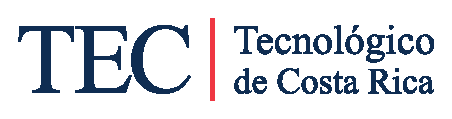
\includegraphics[width=60mm]{Firma_TEC-4}

\par\vspace*{\fill}

{\large\bf{\thesisTitle\par}}

\par\vspace*{\fill}

Informe de Trabajo Final de Graduación para optar por el título de

\thesisAuthorDegree{} en Electrónica con el grado académico de Licenciatura

\par\vspace{20mm}

\thesisAuthor

\vspace*{\fill}

\ifdraft{%
  {Borrador de \thesisDraftDate}%
}{%
  {Cartago, \thesisFinalDate}%
}
\end{center}
\newpage 
\cleardoublepage 


%%% Local Variables: 
%%% mode: latex
%%% TeX-master: "main"
%%% End: 
 % Titlepage in Spanish
  %%% ---------------------------------------------------------------------------
%% titlepage_licce_es.tex
%%
%% Title page
%%
%% $Id: titlepage.tex 1452 2010-07-07 00:55:16Z palvarado $
%% ---------------------------------------------------------------------------
\phantomsection
\pdfbookmark[1]{Portada}{Portada}

\thispagestyle{empty} 

\begin{center}

Tecnológico de Costa Rica

\par\vspace{1ex}

Electronics Engineering Department

\par\vspace{1ex}

Licentiate Degree Program in Electronics Engineering

\par\vspace{20mm}

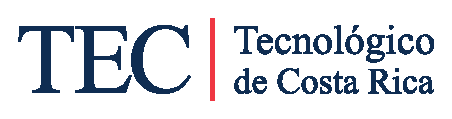
\includegraphics[width=60mm]{Firma_TEC-4}

\par\vspace*{\fill}

{\large\bf{\thesisTitle\par}}

\par\vspace*{\fill}


Final report submitted in partial fulfillment of the requirements

for the degree of Licentiate in Electronics Engineering

\par\vspace{20mm}

\thesisAuthor

\vspace*{\fill}

\ifdraft{%
  {Draft \thesisDraftDate}%
}{%
  {Cartago, \thesisFinalDate}%
}
\end{center}
\newpage 
\cleardoublepage 


%%% Local Variables: 
%%% mode: latex
%%% TeX-master: "main"
%%% End: 
 % Titlepage in English (only if thesis is in En)

  %%% ---------------------------------------------------------------------------
%% titlepage_msc_es.tex
%%
%% Title page
%%
%% $Id: titlepage.tex 1452 2010-07-07 00:55:16Z palvarado $
%% ---------------------------------------------------------------------------
\phantomsection
\pdfbookmark[1]{Portada}{Portada}

\thispagestyle{empty} 

\begin{center}

Tecnológico de Costa Rica

\par\vspace{1ex}

Escuela de Ingeniería Electrónica

\par\vspace{20mm}

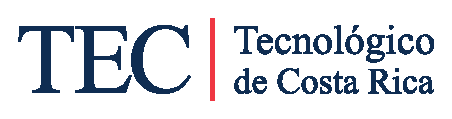
\includegraphics[height=60mm]{Firma_TEC-4}

\par\vspace*{\fill}

{\large\bf{\thesisTitle\par}}

\par\vspace*{\fill}

Documento de tesis sometido a consideración para optar por el grado
académico de Maestría en Electrónica con Énfasis en
%
%Sistemas Embebidos
Procesamiento Digital de Señales
%Microelectrónica
%Sistemas Microelectromecánicos

\par\vspace{20mm}

\thesisAuthor

\vspace*{\fill}

\ifdraft{%
  {Borrador de \thesisDraftDate}%
}{%
  {Cartago, \thesisFinalDate}%
}
\end{center}
\newpage 
\cleardoublepage 


%%% Local Variables: 
%%% mode: latex
%%% TeX-master: "main"
%%% End: 
   % Titlepage in Spanish
  %%% ---------------------------------------------------------------------------
%% titlepage.tex
%%
%% Title page
%%
%% $Id: titlepage.tex 1452 2010-07-07 00:55:16Z palvarado $
%% ---------------------------------------------------------------------------
\phantomsection
\pdfbookmark[1]{Portada}{Portada}

\thispagestyle{empty} 

\begin{center}

Tecnológico de Costa Rica

\par\vspace{1ex}

Escuela de Ingeniería Electrónica

\par\vspace{20mm}

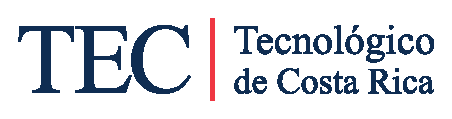
\includegraphics[height=60mm]{Firma_TEC-4}

\par\vspace*{\fill}

{\large\bf{\thesisTitle\par}}

\par\vspace*{\fill}

A thesis submitted in partial fulfillment of the requirements for the
degree of
%
Master of Science in Electronics, Major in 
%
%Embedded Systems
Digital Signal Processing
%Microelectronics
%Microelectromechanical systems

\par\vspace{20mm}

\thesisAuthor

\vspace*{\fill}

\ifdraft{%
  {Draft \thesisDraftDate}%
}{%
  {Cartago, \thesisFinalDate}%
}
\end{center}
\newpage 
\cleardoublepage 


%%% Local Variables: 
%%% mode: latex
%%% TeX-master: "main"
%%% End: 
   % Titlepage in English (only if thesis is in En)

  \thispagestyle{empty}

\rule{\textwidth}{0pt}

\vfill

\ifdraft{%
  El documento
  \href{https://www.tec.ac.cr/sites/default/files/media/doc/requisitos_trabajos_finales_graduacion_2021.pdf}%
  {Requisitos para la entrega de Trabajos Finales de Graduación} a las
  bibliotecas del TEC indica que usted debe incluir la licencia de
  Creative Commons en la página siguiente de la portada.

  Asegúrse entonces de \href{https://creativecommons.org/choose/?lang=es}%
  {elegir la licencia correcta}, y ajustar el texto abajo a su selección.

  Es necesario que
  \href{https://creativecommons.org/about/downloads/}{descargue el
    ícono} correcto en formato vectorial, y lo coloque en el
  directorio \code{fig/}.%
}



\vfill


\framebox[\textwidth]{
  \footnotesize
  \parbox{0.98\textwidth}{%
    \begin{center} %
      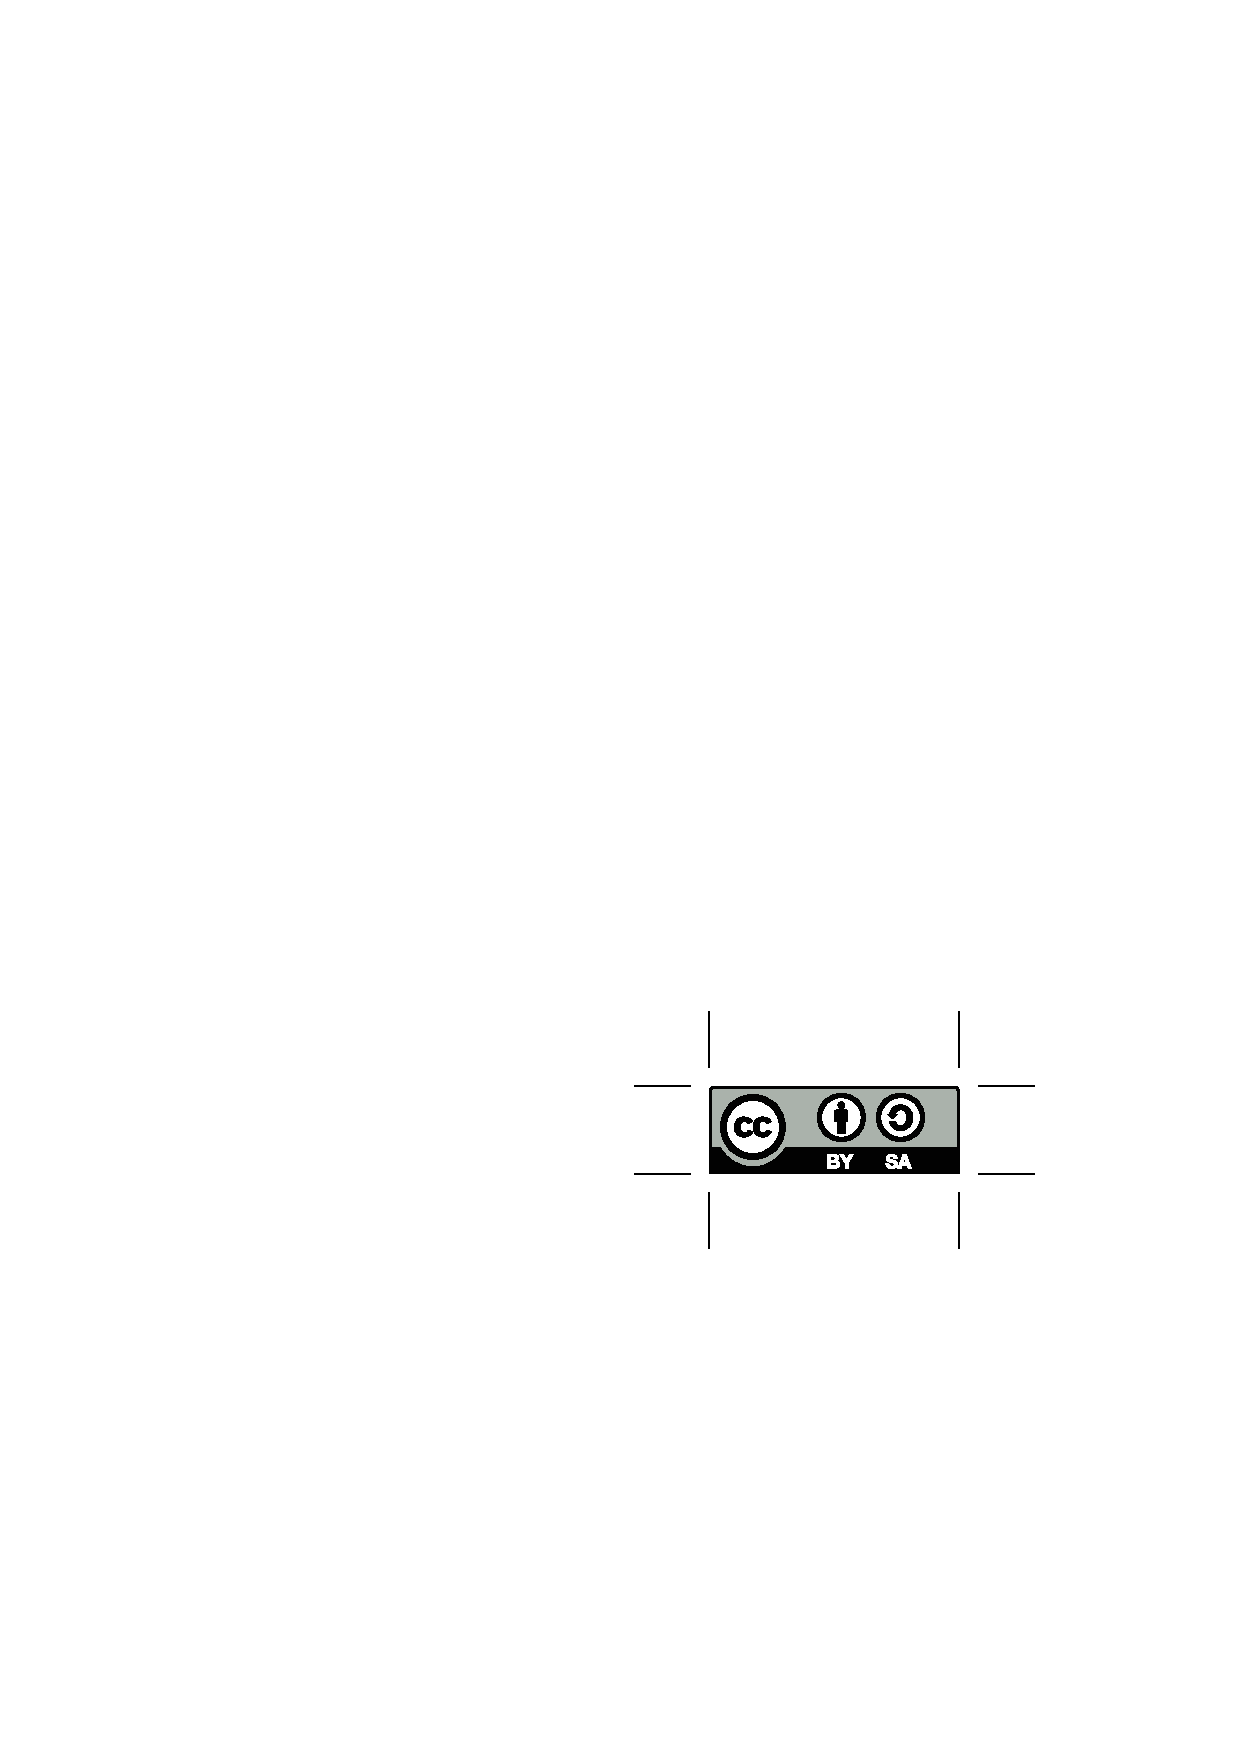
\includegraphics[scale=1]{by-sa} %
    \end{center} %
    
    Este trabajo titulado \emph{\thesisFlatTitle{}} por \thesisAuthor{}, se
    encuentra bajo la Licencia Creative Commons
    \href{http://creativecommons.org/licenses/by-sa/4.0/?ref=chooser-v1}%
    {Atribución-ShareAlike 4.0 International}.
    
    Para ver una copia de esta Licencia, visite
    \url{http://creativecommons.org/licenses/by-sa/4.0/}.\bigskip
    
    \copyright \the\year \hfill%
    \thesisAuthor \hfill%
    \thesisInstitution
  }
}

  
  % Hoja de depuración, con comandos definidos por la plantilla.
  % \phantomsection
\pdfbookmark[1]{Debug}{Debug}

Esta es una página de depuración, para ver todos los comandos
definidos en config.tex

De \verb+babel+ se obtiene que \verb+\tablename+ es \tablename.  Por
lo tanto, en esta versión se usará ``\latabla'' para denotar a cada
``\tabla''.  Ver \tabref{tab:comandostab} para la lista de comandos
existentes.



Este documento es elaborado por \thesisAuthorAddress~\thesisAuthor\
(\thesisAuthorShort) con carné \thesisAuthorTECID, para optar por el
título de \thesisAuthorDegree.

\genderAsesor\ \nameAsesor.

\genderLectorI\ \nameLectorI.

\genderLectorII\ \nameLectorII.

Titulo crudo:

\begin{center}
  \thesisTitle.  
\end{center}

Título aplanado:

``\thesisFlatTitle''.

Palabras clave: \thesisKeywords.

Fecha borrador: \thesisDraftDate

Fecha final: \thesisFinalDate





  
  \thispagestyle{empty}

\rule{10mm}{0pt}

\vfill

Declaro que el presente documento de tesis ha sido realizado enteramente
por mi persona, utilizando y aplicando literatura referente al tema e
introduciendo conocimientos y resultados experimentales propios.

En los casos en que he utilizado bibliografía he procedido a indicar las
fuentes mediante las respectivas citas bibliográficas.  En consecuencia,
asumo la responsabilidad total por el trabajo de tesis realizado y por
el contenido del presente documento.



\vspace*{8mm}

\begin{flushright}
  \thesisAuthor\par
  Cartago, \today\par
  Céd: 1-0123-0456
\end{flushright}

\cleardoublepage

%%% Local Variables: 
%%% mode: latex
%%% TeX-master: "main"
%%% End: 

  %% -------------------------------------------------
  %% Acta y hoja del tribunal
  %%
  %% Asegúrse de que las fechas de defensa de tesis sean las que aparecen
  %% en las actas.
  
  %% Para la Licenciatura en Ingeniería Electrónica:

  %%   Acá se colocan las dos actas como plantillas para ser firmadas
  %%   por el tribunal.

  %%   El acta de aprobación, dependiendo del tribunal, puede dejarla
  %%   en blanco en la tesis, para que el tribunal firme la tesis completa
  %%   sobre esta acta, o, si el tribunal lo decide, extrae la hoja
  %%   para que sea firmada "caligráficamente" por los miembros del tribunal.
  %%   Al acta firmada, en formato PDF (ya sea firmado con tabletas gráficas o
  %%   en papel y escaneada) la integra al documento con el comando para incluir
  %%   el pdf directamente \includepdf{archivo} 
  %% ESTE ARCHIVO DEBE ELIMINARSE DE LA VERSIÓN FINAL

\thispagestyle{empty}

\begin{center}
  \begin{tabular}{c}
    \thesisInstitution \\
    \thesisDepartment \\
    Trabajo Final de Graduación \\
    Acta de Aprobación
  \end{tabular}
\end{center}

\vfill

\begin{center}
  \begin{tabular}{c}
    Defensa de Trabajo Final de Graduación \\
    Requisito para optar por el título de \thesisAuthorDegree\ en Electrónica\\
    Grado Académico de Licenciatura
  \end{tabular}
\end{center}

\vfill

%% \thesisAuthorAddress, \thesisAuthor y \thesisTitle están en main.tex
El Tribunal Evaluador aprueba la defensa del trabajo final de graduación
denominado \textsl{\thesisFlatTitle{}}, realizado por
%
\thesisAuthorAddress\ \thesisAuthor\ %
%
y, hace constar que cumple con las normas
establecidas por la \thesisDepartment{} del \thesisInstitution{}.

\vfill

\begin{center}
 Miembros del Tribunal Evaluador
\end{center}

\vfill

\begin{center}
  \begin{tabularx}{\textwidth}{cXc}
    \rule{0.45\textwidth}{0.5pt} && \rule{0.45\textwidth}{0.5pt} \\
    \nameLectorI                 && \nameLectorII \\
    \genderLectorI               && \genderLectorII
  \end{tabularx}
  
  \vspace{10mm}

  \begin{tabular}{c}
    \rule{0.45\textwidth}{0.5pt} \\
    \nameAsesor \\
    \genderAsesor
  \end{tabular}
\end{center}

\vfill

\begin{center}
  Cartago, \ifdraft{\thesisDraftDate}{\thesisFinalDate}\par
\end{center}

\cleardoublepage

%%% Local Variables: 
%%% mode: latex
%%% TeX-master: "main"
%%% End: 
  % Remover en versión final
  %\includepdf{acta_aprob_firmada} % Incluir el acta firmada acá.

  %% El acta de evaluación usualmente la extrae del documento y
  %% la entrega al tribunal para que sea firmada, y ellos la hacen
  %% llegar al profesor del curso de TFG.  Ese documento no
  %% debe aparecer en la tesis final, así que esta línea deberá
  %% comentarla en la versión final:
  %% ESTE ARCHIVO DEBE ELIMINARSE DE LA VERSIÓN FINAL


\thispagestyle{empty}

\begin{center}
  \begin{tabular}{c}
    \thesisInstitution \\
    \thesisDepartment \\
    Trabajo Final de Graduación \\
    Tribunal Evaluador \\
    Acta de Evaluación
  \end{tabular}
\end{center}

\vfill

\begin{center}
  \begin{tabular}{c}
    Defensa del Trabajo Final de Graduación \\
    Requisito para optar por el título de \thesisAuthorDegree\ en Electrónica\\
    Grado Académico de Licenciatura
  \end{tabular}
\end{center}

\vfill

%% Configurar todo en config.tex
\begin{center}

  Estudiante:%
  \qquad \textbf{\thesisAuthor}%
  \qquad Carné: \thesisAuthorTECID

  \vspace*{2ex}

  \setlength\tabcolsep{0pt}
  \begin{tabular}{p{.25\textwidth}p{.73\textwidth}}
    Nombre del proyecto: & \textsl{\thesisFlatTitle}
  \end{tabular}
\end{center}
\vspace{5mm}

\vfill

Los miembros de este Tribunal hacen constar que este trabajo final de
graduación ha sido aprobado y cumple con las normas establecidas por
la \thesisDepartment{} del \thesisInstitution{} y es merecedor de la
siguiente calificación:

\vfill

\begin{center}
  Nota del Trabajo Final de Graduación: \rule{25mm}{0.5pt}
\end{center}

\vfill

\begin{center}
 Miembros del Tribunal Evaluador
\end{center}

\vfill

% Defina con \setLector* en main.tex (líneas 87-89) los lectores y asesor
\begin{center}
  \begin{tabularx}{\textwidth}{cXc}
    \rule{0.45\textwidth}{0.5pt} && \rule{0.45\textwidth}{0.5pt} \\
    \nameLectorI                 && \nameLectorII \\
    \genderLectorI               && \genderLectorII
  \end{tabularx}
  
  \vspace{10mm}

  \begin{tabular}{c}
    \rule{0.45\textwidth}{0.5pt} \\
    \nameAsesor \\
    \genderAsesor
  \end{tabular}
\end{center}

\vfill

\begin{center}
  Cartago, \ifdraft{\thesisDraftDate}{\thesisFinalDate}\par
\end{center}

\cleardoublepage

%%% Local Variables: 
%%% mode: latex
%%% TeX-master: "main"
%%% End: 
   % >> Remover en versión final <<
    
  %% Para la maestría en electrónica:
  %%% ESTE ARCHIVO DEBE ELIMINARSE DE LA VERSIÓN FINAL

\thispagestyle{empty}

\begin{center}
  \begin{tabular}{c}
    \thesisInstitution \\
    \thesisDepartment \\
    Proyecto de Graduación \\
    Tesis de Maestría \\
    Tribunal Evaluador
  \end{tabular}
\end{center}

\vfill

Tesis de maestría defendida ante el presente Tribunal Evaluador como
requisito para optar por el grado académico de maestría, del
\thesisInstitution.

\vfill

\vspace*{20mm}
\begin{center}
 Miembros del Tribunal
\end{center}
\vspace*{8mm}

\vfill

\begin{center}
  \begin{tabularx}{\textwidth}{cXc}
    \rule{0.45\textwidth}{0.5pt} && \rule{0.45\textwidth}{0.5pt} \\
    \nameLectorI                 && \nameLectorII \\
    \genderLectorI               && \genderLectorII
  \end{tabularx}
  
  \vspace{10mm}

  \begin{tabular}{c}
    \rule{0.45\textwidth}{0.5pt} \\
    \nameAsesor \\
    \genderAsesor
  \end{tabular}
\end{center}

\vfill


Los miembros de este Tribunal dan fe de que la presente tesis de
maestría ha sido aprobada y cumple con las normas establecidas por la
\thesisDepartment.

\vfill

\begin{center}
  Cartago, \today\par
\end{center}

\cleardoublepage

%%% Local Variables: 
%%% mode: latex
%%% TeX-master: "main"
%%% End: 
  % Remover en versión final
  %%% ESTE ARCHIVO DEBE ELIMINARSE DE LA VERSIÓN FINAL


\thispagestyle{empty}

\begin{center}
  \begin{tabular}{c}
    \thesisInstitution \\
    \thesisDepartment \\
    Tesis de Maestría \\
    Acta de Evaluación
  \end{tabular}
\end{center}

\vfill

Tesis de maestría defendida ante el presente Tribunal Evaluador como
requisito para optar por el grado académico de maestría, del
\thesisInstitution.

\vspace*{15mm}

%% Configurar todo en config.tex
\begin{center}
  Estudiante: \thesisAuthor
\end{center}

\vfill

\begin{center}
  Nombre del Proyecto: \thesisFlatTitle}
\end{center}

\vspace*{20mm}
\begin{center}
 Miembros del Tribunal Evaluador
\end{center}
\vspace*{8mm}

\vfill

% Los nombres de lectores y asesor se definen en el archivo main.tex
\begin{center}
  \begin{tabularx}{\textwidth}{cXc}
    \rule{0.45\textwidth}{0.5pt} && \rule{0.45\textwidth}{0.5pt} \\
    \nameLectorI                 && \nameLectorII \\
    \genderLectorI               && \genderLectorII
  \end{tabularx}
  
  \vspace{10mm}

  \begin{tabular}{c}
    \rule{0.45\textwidth}{0.5pt} \\
    \nameAsesor \\
    \genderAsesor
  \end{tabular}
\end{center}

\vfill

Los miembros de este Tribunal dan fe de que la presente tesis de
maestría ha sido aprobada y cumple con las normas establecidas por la
\thesisDepartment.

\vfill

\begin{center}
  Nota final de la Tesis de Maestría: \rule{3cm}{0.5pt}
\end{center}
\vfill

\begin{center}
  Cartago, \today\par
\end{center}

\cleardoublepage

%%% Local Variables: 
%%% mode: latex
%%% TeX-master: "main"
%%% End: 
   % Remover en versión final
  %% -------------------------------------------------
  \chapter*{Resumen}
\thispagestyle{empty}

Este proyecto se centra en el desarrollo de flujos de trabajo robustos para la implementación de software en sistemas de computadoras de guía, navegación y control (GNC) espaciales. El primer paso consiste en seleccionar una plataforma de hardware óptima para diseñar un modelo de ingeniería de una computadora de navegación espacial. Sobre esta base, se establecerán procesos para el prototipado de algoritmos de control de orientación y navegación, con un enfoque especial en sistemas hardware-in-the-loop. Estos sistemas permitirán una validación más realista de los algoritmos en condiciones espaciales simuladas.
Además, se explorarán casos de uso aplicados a un sistema de navegación y control a través del desarrollo de una aplicación de referencia. Esta aplicación se basará en una Unidad de Medida Inercial (IMU) y un controlador PID, demostrando la interacción y el rendimiento de los componentes involucrados. Este enfoque integral busca optimizar la implementación de software en sistemas GNC espaciales, mejorando significativamente su eficiencia y confiabilidad.

\bigskip

%% Defina las palabras clave con defKeywords en config.tex:
\textbf{Palabras clave:} \thesisKeywords

\clearpage
\chapter*{Abstract}
\thispagestyle{empty}

This project focuses on developing robust workflows for the implementation of software in space guidance, navigation, and control (GNC) computers. The first step involves selecting an optimal hardware platform to design an engineering model of a space navigation computer. Based on this foundation, processes will be established for prototyping orientation and navigation control algorithms, with a special emphasis on hardware-in-the-loop systems. These systems will enable a more realistic validation of the algorithms under simulated space conditions.
Additionally, use cases applied to a navigation and control system will be explored through the development of a reference application. This application will be based on an Inertial Measurement Unit (IMU) and a PID controller, demonstrating the interaction and performance of the involved components. This comprehensive approach aims to optimize the implementation of software in space GNC systems, significantly improving their efficiency and reliability.

\bigskip

\textbf{Keywords:} GNC, Systems, embedded, processor, framework, model to model transformation, embedded code, MATLAB, simulink, containers

\cleardoublepage

%%% Local Variables: 
%%% mode: latex
%%% TeX-master: "main"
%%% End: 

  \vspace*{0.4\textheight}
% No debe confundirse la dedicatoria con el agradecimiento.
% La dedicatoria solo tiene una línea corta de la persona a quien se dedica.

{\hfill{\Large{\emph{a mis queridos padres}}}}

  \chapter*{Agradecimientos}
\thispagestyle{empty}

El resultado de este trabajo no habría sido posible sin el apoyo incondicional de 
Johan Carvajal Godínez, quien siempre mostró una gran disponibilidad para cooperar 
y asegurarse de que este proyecto se llevara a cabo con éxito. También quiero expresar
mi gratitud al laboratorio de sistemas espaciales y a todos sus 
integrantes por su valiosa contribución.

\vspace*{1cm}

\thesisAuthor

Cartago, \today

\cleardoublepage

%%% Local Variables: 
%%% mode: latex
%%% TeX-master: "paMain"
%%% End: 


  %----------------------------------------------------------------------------
  \frontmatter
  %----------------------------------------------------------------------------
  \pagestyle{fancy}
  \pagenumbering{roman}

  \pdfbookmark[1]{Indice General}{Indice General}

  \parskip0ex                           % space between paragraphs

  \tableofcontents                      % Table of contents
  \listoffigures                        % List of figures
  \listoftables                         % List of tables
  \lstlistoflistings
\ifdraft{%
  % todo's                              % TODOs
  \listoftodo
}{%
}

  %% ---------------------------------------------------------------------------
%% paNotation.tex
%%
%% Notation
%%
%% $Id: paNotation.tex,v 1.15 2004/03/30 05:55:59 alvarado Exp $
%% ---------------------------------------------------------------------------

\cleardoublepage
\renewcommand{\nomname}{Lista de símbolos y abreviaciones}
\setlength{\nomitemsep}{-\parsep}

%%
% Commands required for the nomenclature groups
%
% There are following prefix forms:
%  a   abbreviation    \syma[key]{symbol}{description}
%  g   general         \symg[key]{symbol}{description}
%%

\renewcommand{\nomgroup}[1]{%
  \ifthenelse{\equal{#1}{G}}{\section*{\hspace*{-\leftmargin}Notación general}}{}%
  \ifthenelse{\equal{#1}{A}}{\section*{\hspace*{-\leftmargin}Abreviaturas y Siglas}}{}%
}

\newcommand{\syma}[3][foo]{%
  \ifthenelse{\equal{#1}{foo}}%
  {\nomenclature[A]{#2}{#3}}{\nomenclature[A#1]{#2}{#3}}}
\newcommand{\symg}[3][foo]{%
  \ifthenelse{\equal{#1}{foo}}%
  {\nomenclature[G]{#2}{#3}}{\nomenclature[G#1]{#2}{#3}}}

%%
% Símbolos en la notación general
% (es posible poner la declaración en el texto
%%


\symg[t]{$\sys{\cdot}$}{Transformación realizada por un sistema.}
\symg[yscalar]{$y$}{Escalar.}
\symg[zconjugado]{$\conj{z}$}{Complejo conjugado de $z$.}
\symg[rcomplexreal]{$\Re(z)$ o $z_{\Re}$}{Parte real del número complejo $z$.}
\symg[icompleximag]{$\Im(z)$ o $z_{\Im}$}{Parte imaginaria del número
                                        complejo $z$.}
\symg[jimaginario]{$j$}{$j=\sqrt{-1}$.}
\symg[xvector]{$\vct{x}$}{Vector. \newline\hspace{1mm}%
  $\vct{x}=\left[ x_1 \; x_2 \; \ldots \; x_n \right]^T =
  \begin{bmatrix}
    x_1 \\ x_2 \\ \vdots \\ x_n
  \end{bmatrix}$}

\symg[mmatrix]{$\mat{A}$}{Matriz. \newline\hspace{1mm}%
  $\mat{A} =
  \begin{bmatrix}
    a_{11} & a_{12} & \cdots & a_{1m}\\
    a_{21} & a_{22} & \cdots & a_{2m}\\
    \vdots & \vdots & \ddots & \vdots\\
    a_{n1} & a_{n2} & \cdots & a_{nm}\\
  \end{bmatrix}$}

\symg[C]{$\setC$}{Conjunto de los números complejos.}

%%
% Algunas abreviaciones
%%

\syma{PCA}{Análisis de componentes principales}
\syma{WSN}{Redes Inalámbricas de Sensores}
\syma{ASM}{Modelos Activos de Forma}

\printnomenclature[20mm]

%%% Local Variables:
%%% mode: latex
%%% TeX-master: "paMain"
%%% End:
                    % Abbreviation

  \parskip1.3ex                         % space between paragraphs

  %----------------------------------------------------------------------------
  \mainmatter
  %----------------------------------------------------------------------------
  % where to look for graphics
  \graphicspath{{./}{./fig/}}
  %\pagenumbering{arab}

  % Main files
  %% ---------------------------------------------------------------------------
%% intro.tex
%%
%% Introduction
%%
%% $Id: intro.tex 1477 2010-07-28 21:34:43Z palvarado $
%% ---------------------------------------------------------------------------

\chapter{Introducción}
\label{chp:intro}

\section{Proceso de diseño de los sistemas de Guía, Navegación y Control espacial}

La implementacion de sistemas GNC en sistemas embebidos, conlleva una combinacion de
hardware y software especializado, por un lado, los microcontroladores son los encargados de
gestionar los clculos, mientras que los sensores proporcionan distintos tipos de datos por medio
de las entradas. Por otro lado, los sistemas en tiempo real garantizan la respuesta en el momento
requerido. Las aplicaciones de estos se pueden observar en drones, satelites y sondas espaciales
[4].

Como se menciono anteriormente los sistemas GNC son fundamentales en las misiones es-
paciales, estan encargados de determinar la trayectoria optima para cumplir los objetivos de
la mision, ademas de calcular la secuencia de maniobras necesarias, determinar la posicion,
velocidad y orientacion, tambien se encargan de aplicar las acciones correctivas necesarias para
mantener la trayectoria [15].

\subsection{Requerimientos de los sistemas}

Los requerimientos de los sistemas GNC incluyen: precision para determinar la posicion
y orientacion del vehiculo con gran exactitud, robustez para funcionar de manera confiable
y tolerar fallos o perturbaciones generadas por el entorno, autonomia para poder operar sin
depender de la intervencion humana, flexibilidad para adaptarse a diferentes fases de la mision
y un bajo consumo de potencia para minimizar el uso de los recursos limitados a bordo.

Para cumplir con los requerimientos mencionados anteriormente se debe definir con precision
los requerimientos del sistema, como la precision necesaria para determinar la posicion del
vehiculo, la robustez del sistema para resistir fallos, las restricciones energeticas y de recursos
computacionales a bordo. Una vez solventados estos requerimientos el sistema se plantea bajo
una arquitectura modular la cual divide el sistema en bloques independientes para las funciones
de guia, navegacion y control, facilitando el desarrollo, prueba y mantenimiento [1].

\section{Sistemas embebidos para los sistemas GNC}
El uso de sistemas embebidos ha transformado la navegación y el control aeroespacial. Estos sistemas 
integran hardware y software, permitiendo el procesamiento de datos en tiempo real, fundamental para 
la navegación precisa y el control de vuelo. Los sistemas embebidos gestionan sensores que recopilan 
información sobre altitud, velocidad y posición, permitiendo a pilotos y sistemas automáticos tomar 
decisiones rápidas y fundamentadas. Esta capacidad de respuesta es esencial en entornos cambiantes, 
como la aviación o el lanzamiento de cohetes.

Además, los sistemas embebidos facilitan la integración de múltiples funciones en un solo dispositivo,
 reduciendo el peso y volumen de los equipos a bordo, un factor crucial en la industria aeroespacial. 
 Por ejemplo, en los sistemas de control de vuelo, los microcontroladores y procesadores embebidos pueden
  gestionar desde la navegación hasta la comunicación y el monitoreo de sistemas críticos, todo desde una 
  única unidad. Esta integración mejora la eficiencia del espacio y minimiza la posibilidad de fallos al 
  reducir el número de componentes individuales que podrían fallar.

Finalmente, la implementación de sistemas embebidos ha permitido avances significativos en la automatización 
y la inteligencia artificial aeroespacial. Los algoritmos embebidos procesan datos de manera eficiente, permitiendo 
la navegación autónoma y el control de vehículos sin intervención humana, especialmente relevante en misiones
 espaciales con comunicación limitada. Los sistemas embebidos mejoran la seguridad y eficiencia de las operaciones 
 aeroespaciales, abriendo nuevas posibilidades para la exploración y el desarrollo de tecnologías futuras en este campo.

\subsection{Marco de Trabajo Yocto}
El Yocto Project es una iniciativa de código abierto que proporciona un conjunto de herramientas y recursos para crear 
sistemas operativos Linux personalizados, especialmente diseñados para dispositivos embebidos. Su objetivo principal es 
facilitar el desarrollo de software y la integración de componentes en una amplia variedad de hardware, permitiendo a los 
desarrolladores construir imágenes de sistema adaptadas a sus necesidades específicas. Utiliza BitBake, una herramienta que 
permite definir recetas para la construcción y empaquetado de software, lo que otorga gran flexibilidad y personalización. 
Además, soporta múltiples arquitecturas de hardware, como ARM, x86, MIPS y PowerPC, lo que lo hace adecuado para diferentes 
dispositivos, desde microcontroladores hasta sistemas más complejos. Al fomentar la reutilización de componentes y contar con 
una comunidad activa que contribuye con mejoras y documentación, el Yocto Project se convierte en una solución ideal para el 
desarrollo de sistemas operativos en aplicaciones de IoT, electrónica de consumo y automatización industrial.

\section{Donde se ubica dentro del flujo de control}
Diagrama profe Johan (ver en proxima reunion)

\section{Hardware en el loop}
El Hardware en el loop es una tecnica fundamental en el desarrollo de sistemas GNC, ya que,
permite simular el comportamiento del hardware en tiempo real, facilitando para los desarrolla-

dores la prueba y validacion del software sin requerir el hardware fisico, es esta forma permite
probar de forma exhaustiva el software asegurando el funcionamiento del hardware simulado y
permite la validacion de todo el sistema antes de su implementacion final. Esta implementacion
genera una mayor precision en las pruebas, la posibilidad de validar la autonomia del sistema,
ademas de reducir significativamente el tiempo y los costos de implementacion y prueba del
hardware. En resumen, es una tecnica esencial en el desarrollo de sistemas GNC espaciales, per-
mitiendo una validacion integral y eficiente de estos complejos sistemas antes de su despliegue
en misiones reales [19] [21].



\section{Objetivos y estructura del documento}

\index{objetivos}

El objetivo principal de este proyecto es desarrollar un conjunto de flujos de trabajo para la implementacion de software a bordo de
computadoras de guia, navegacion y control espacial. Para lograr este objetivo se persiguen tres objetivos
especificos. El primero consiste en Identificar una plataforma de hardware para el desarrollo de un modelo de ingenieria de
una computadora de navegacion espacial.

El segundo se encarga de Establecer flujos de trabajo para el prototipado de algoritmos de control de orientacion
y navegacion para aplicaciones espaciales con hardware en el loop. Y por ultimo el tecero consiste en Evaluar los casos de uso de una computadora de navegacion y control espacial mediante
la implementacion de una aplicacion de referencia demostrativa (caso de la IMU)


Este documento incluye lo siguiente: en el capitulo 2 se presenta el marco teorico, donde se
esbozan los fundamentos de la propuesta realizada. En el capitulo 3 se detalla la solucion
propuesta y el modelo implementado para la solucion del problema. En el capitulo 4 se
presentan los resultados obtenidos. Por ultimo, el capitulo 5 se presenta las conclusiones
de la investigacion y trabajo realizado, asi como recomendaciones y trabajo a futuro por
desarrollar.

%%% Local Variables: 
%%% mode: latex
%%% TeX-master: "main"
%%% End: 

  \chapter{Marco teórico}
\label{ch:marco}

En este capítulo se presentan los conceptos teóricos que subyacen la propuesta de desarrollo de un conjunto de flujos de trabajo para la implementación de software 
a bordo de computadoras de guía, navegación y control espacial. La información expuesta se deriva tanto de conocimientos propios como información bibliográfica.

\section{Estimación}
La estimación implica el uso de modelos matemáticos y algoritmos para calcular las variables de estado del sistema. Estas variables son esenciales para comprender 
el comportamiento del sistema y para tomar decisiones informadas sobre su control. La estimación puede realizarse de dos maneras:

\begin{itemize}
    \item Lazo abierto: En este enfoque, se utilizan modelos de estimación predefinidos sin retroalimentación, lo que significa que las estimaciones no se ajustan en función
    de las mediciones reales.
    \item Lazo cerrado: Este método ajusta las estimaciones en función de las mediciones reales y las salidas del sistema, lo que permite una mayor precisión y adaptabilidad.
\end{itemize}

Esta es crucial en aplicaciones donde las mediciones directas son difíciles o costosas de obtener, por ejemplo en los sistemas hidráulicos, la estimación de variables de 
estado permite optimiza el rendimiento y la eficiencia del sistema, asegurando que se mantengan las condiciones deseadas a pesar de las perturbaciones externas o errores en las 
mediciones \cite{Merchn2019EvaluacinDM}. La estimación es un componente clave en los sistemas de control, ya que facilita la comprensión y el manejo de sistemas complejos. 
Su implementación permite una operación más eficiente y efectiva, mejorando su capacidad de respuesta ante diversa condiciones operativas \cite{Mesa2020EstimacinDV}.

\section{Control}
Como se mencionó anteriormente la estimación es un componente clave en los sistemas de control, ya que este se enfoca en el desarrollo y diseño de sistemas capaces de regular 
y controlar variables de un proceso de manera autónoma. Estos sistemas utilizan sensores, actuadores y algoritmos de control para mantener las variables de interés dentro de los 
rangos permitidos, mejorando de esta forma la eficiencia, precisión y confiabilidad de los procesos. Su aplicación abarca desde sistemas espaciales hasta biorreactores y sistemas
de iluminación. 


\section{Procesadores embebidos}

Los procesadores embebidos son microprocesadores especializados en tareas dentro de un sistema más complejo. A diferencia de los procesadores de propósito general, estos están 
optimizados para ofrecer eficiencia energética, un tamaño compacto y costo reducido. Algunas de las características de los procesadores embebidos se presentan a continuación:

\begin{itemize}
    \item Integración de periféricos: Incorporan periféricos específicos de la aplicación en un único chip, incluyendo temporizadores, puertos de entrada/salida y controladores 
    de memoria.
    \item Arquitecturas de bajo Consumo: Diseñados para maximizar la duración de la batería en dispositivos portátiles, lo que es esencial para la operatividad de dispositivos 
    móviles.
    \item Tamaño compacto: Su diseño permite reducir costos y facilitar la integración en espacios limitados, lo que los hace ideales para aplicaciones donde el espacio es 
    crítico.
    \item Capacidad de respuesta en tiempo real: Pueden responder a eventos externos de manera predecible y determinista, lo que es crucial en aplicaciones que requieren una respuesta rápida y precisa.
\end{itemize}

\subsection{Cortex-A9}

Los procesadores embebidos basados en la arquitectura ARM Cortex-A9 se utilizan en aplicaciones de alto rendimiento y capacidades avanzadas de procesamiento.
Aunque esta arquitectura no es un procesador embebido, sino más bien una familia de núcleos de procesador diseñado por ARM Holdings, los SoC que incorporan
estos núcleos han demostrado ser una solución popular para aplicaciones embebidas \cite{Schwiegelshohn2014DesignOA}. Algunas de sus características son : 

\begin{itemize}
    \item Arquitectura de 32 bits basada en ARMv7-A.
    \item Alto rendimiento adecuado para aplicaciones exigentes como sistemas operativos embebidos, procesamiento multimedia y gráficos.
    \item Características avanzadas como unidades de coma flotante, unidades de procesamiento NEON para procesamiento multimedia y soporte para virtualización.
\end{itemize}

Algunos SoC que incorporan núcleos Cortex-A9 son:

\begin{itemize}
    \item Nvidia Tegra 3: Combina cuatro núcleos Cortex-A9 y una GPU.
    \item Texas Instruments OMAP 4: Familia de SoC que combina núcleos Cortex-A9 y DSP.
    \item Xilinx Zynq-7000: Integra núcleos Cortex-A9 con lógica programable FPGA.
\end{itemize}

\subsection{Tarjeta de desarrollo ZedBoard}

La ZedBoard es una tarjeta de desarrollo basada en el Xilinx Zynq-7000 que como se mencionó anteriormente integra núcleos Cortex-A9 con la lógica programable 
para Field Programmable Gate Array,por sus siglas en ingles (FPGA). Esta plataforma es ideal para prototipar aplicaciones en el ámbito de sistemas embebidos. La tabla \ref{tab:zedboard} 
resume las especificaciones que posee la tarjeta de desarrollo ZedBoard.


\begin{figure}[h!]
    \centering
    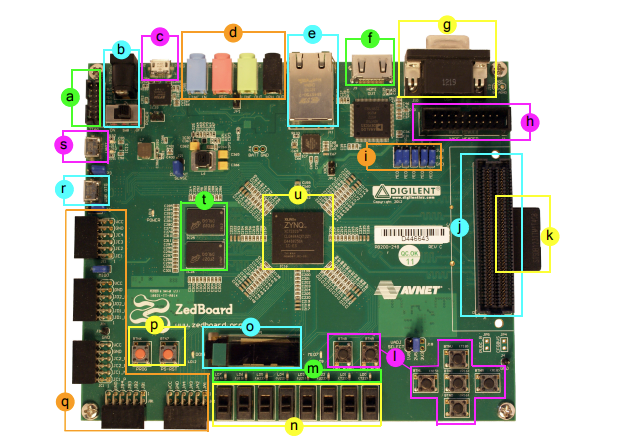
\includegraphics[width=0.8\textwidth]{fig/teorico/zedboard_raw.png}
    \caption{Tarjeta de desarrollo Zedboard}
    \label{fig:zedboard_raw_info}
\end{figure}

Como se pudo observar en \ref{fig:zedboard_raw_info}, esta tarjeta de desarrollo cuenta con los puertos de conexión que se mencionan en la Tabla \ref{tab:puertos_yocto}: 

\begin{table}[htbp!]
    \caption{Puertos de entrada y salida de la plataforma de desarrollo Zedbord}
    \label{tab:puertos_yocto}
    \resizebox{\textwidth}{!}{%
    \begin{tabular}{|l|l|ll}
    \hline
    Identificador & Descripción                     & \multicolumn{1}{l|}{Identificador} & \multicolumn{1}{l|}{Descripción}      \\ \hline
    a             & Conector JTAG Xilinx            & \multicolumn{1}{l|}{l}             & \multicolumn{1}{l|}{Pulsadores}       \\ \hline
    b & Entrada de voltaje y   interruptor de encendido & \multicolumn{1}{l|}{m} & \multicolumn{1}{l|}{LEDs}                                 \\ \hline
    c             & USB-JTAG para   programación    & \multicolumn{1}{l|}{n}             & \multicolumn{1}{l|}{Interruptores}    \\ \hline
    d             & Puertos de audio                & \multicolumn{1}{l|}{o}             & \multicolumn{1}{l|}{Pantalla OLED}    \\ \hline
    e & Puerto de ethernet                              & \multicolumn{1}{l|}{p} & \multicolumn{1}{l|}{Botones de   programación y reinicio} \\ \hline
    f             & Puerto HDMI (Salida   de video) & \multicolumn{1}{l|}{q}             & \multicolumn{1}{l|}{Conectores Pmod}  \\ \hline
    g & Puerto VGA (Salida de   video)                  & \multicolumn{1}{l|}{r} & \multicolumn{1}{l|}{USB OTG para   perifericos}           \\ \hline
    h             & Puerto XADC                     & \multicolumn{1}{l|}{s}             & \multicolumn{1}{l|}{USB UART}         \\ \hline
    i             & Jumpers de   configuración      & \multicolumn{1}{l|}{t}             & \multicolumn{1}{l|}{Memoria DDR3}     \\ \hline
    j             & Conector FCM                    & \multicolumn{1}{l|}{u}             & \multicolumn{1}{l|}{Dispositivo Zynq} \\ \hline
    k             & Entrada para tarjeta   SD       &                                    &                                       \\ \cline{1-2}
    \end{tabular}%
    }
\end{table}

\begin{table}[h!]
    \caption{Especificaciones generales de la tarjeta de desarrollo ZeadBoard}
    \label{tab:zedboard}
    \resizebox{\textwidth}{!}{%
    \begin{tabular}{|l|l|}
    \hline
    \multicolumn{1}{|c|}{\textbf{Especificación}} & \multicolumn{1}{c|}{\textbf{Detalles}} \\ \hline
    \textbf{Procesador}             & Xilinx Zynq-7000 (XC7Z020)                         \\ \hline
    \textbf{Núcleos de Procesador}  & ARM Cortex-A9 de doble núcleo                      \\ \hline
    \textbf{Memoria DDR3}           & 512 MB                                             \\ \hline
    \textbf{Memoria Flash}          & 256 MB QSPI                                        \\ \hline
    \textbf{Almacenamiento}         & Tarjeta SD de 4 GB                                 \\ \hline
    \textbf{Conectividad}           & Ethernet (10/100/1000 Mbps), USB OTG 2.0, USB-UART \\ \hline
    \textbf{Salidas de Video}       & HDMI (1080p), VGA de 8 bits, OLED 128x32           \\ \hline
    \textbf{Audio}                  & Códec de audio I2S                                 \\ \hline
    \textbf{Puertos GPIO}           & 54 pines GPIO                                      \\ \hline
    \textbf{Interfaz de JTAG}       & Soporte para programación y depuración             \\ \hline
    \textbf{Dimensiones}            & 10.2 cm x 6.4 cm                                   \\ \hline
    \textbf{Fuente de Alimentación} & 5V a través de conector de alimentación            \\ \hline
    \textbf{Sistema Operativo}      & Soporte para Linux y otros sistemas embebidos      \\ \hline
    \textbf{Expansión}              & Conectores Pmod y FMC para módulos adicionales     \\ \hline
    \end{tabular}%
    }
\end{table}

Además de esto algunas especificaciones de la plataforma de desarrollo son mencionadas en \ref{tab:zedboard}. Por otro lado la ZedBoard es una plataforma de desarrollo altamente versátil que se destaca por su capacidad para ejecutar sistemas operativos como Linux, lo que la convierte en una opción ideal para proyectos de diseño y desarrollo de sistemas embebidos. Además de su compatibilidad con Linux, como se mencionó anteriormente la ZedBoard cuenta con especificaciones técnicas que la hacen destacar en el ámbito del desarrollo. Entre ellas se incluyen un procesador ARM Cortex-A9, una FPGA. 

\section{Marcos de trabajo}

Los marcos de trabajo en sistemas embebidos son conjuntos de herramientas y bibliotecas que facilitan el desarrollo de aplicaciones en estos 
sistemas. Estos proporcionan una estructura que permite abordar los desafíos específicos que presentan los sistemas embebidos.

Los sistemas embebidos interactúan con su entorno físico, lo que requiere un diseño que no solo considere los resultados de las operaciones, 
sino también el cumplimiento de plazos y restricciones específicas. En este contexto, las propiedades no funcionales, como el consumo energético, 
la latencia, la fiabilidad y el manejo de recursos, son críticas para el diseño y optimización del rendimiento general del sistema \cite{Marugn2017SimulacinYV}. Los frameworks 
juegan un papel fundamental al proporcionar herramientas y bibliotecas predefinidas, permitiendo a los desarrolladores centrarse en la lógica de la 
aplicación en lugar de lidiar con los detalles de bajo nivel del hardware, lo que acelera el proceso de desarrollo y reduce la posibilidad de errores. 
Ejemplos de frameworks populares en sistemas embebidos incluyen Robot Operating System (ROS), utilizado en aplicaciones de robótica, y FreeRTOS, 
un sistema operativo de tiempo real diseñado para microcontroladores y sistemas embebidos \cite{HerreraLpez2023EntornoDT}.

\subsection{YOCTO}\label{subsec:yocto}

Yocto es un marco de trabajo o bien del inglés (framework) popular utilizado en el desarrollo de sistemas embebidos, especialmente en la creación de distribuciones de Linux 
personalizadas para hardware específico. Yocto utiliza un proceso de construcción cruzada, lo que significa que el código se compila en una plataforma diferente 
a la que se ejecutará, permitiendo que el código se optimice para el hardware específico del sistema embebido \cite{Leppakoski2013FrameworkFI}.

\begin{figure}[h!]
    \centering
    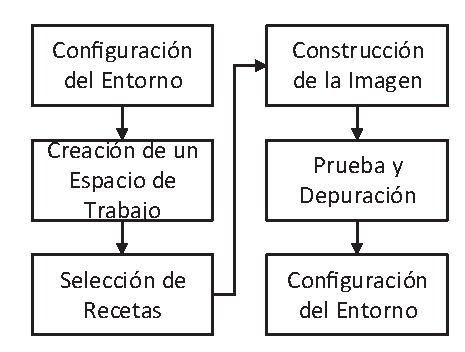
\includegraphics[width=0.5\textwidth]{fig/teorico/Flujo de trabajo de yocto.pdf}
    \caption{Flujo de trabajo Yocto Project}
    \label{fig:yocto_project_workflow}
\end{figure}

Una de las principales ventajas de Yocto es su flexibilidad en la configuración del sistema, permitiendo a los desarrolladores seleccionar paquetes específicos, 
configurar opciones de compilación y personalizar el sistema operativo según sus necesidades. Además, Yocto fomenta la reutilización de código a través de capas, 
que son colecciones de recetas, configuraciones y parches que se pueden agregar o eliminar fácilmente del flujo de trabajo de construcción \cite{Leppakoski2013FrameworkFI}.

\section{MATLAB}
MATLAB es un software de cálculo técnico desarrollado por MathWorks, ampliamente utilizado en diversas áreas de la ciencia y la ingeniería. Proporciona un entorno interactivo para el desarrollo de algoritmos, análisis de datos, visualización y cálculo numérico. Su facilidad para trabajar con vectores y matrices lo distingue de otros sistemas de cálculo \cite{PealozaLuna2022SimulacinDU}. Es comúnmente utilizado para simular sistemas eléctricos, como convertidores DC/DC, y realizar análisis numéricos en problemas complejos \cite{OrdezGarca2022MatlabCU}. 

MATLAB juega un papel crucial en el desarrollo de sistemas de control aeroespaciales, facilitando la simulación, modelado y control de vehículos aéreos no tripulados (UAV) y otros sistemas relacionados.MATLAB, junto con Simulink, permite el modelado cinemático y dinámico de UAVs. Esto incluye la programación y control de sus movimientos, como cabeceo y guiñada, utilizando motores de corriente directa y encoders ópticos para medir su posición \cite{Senz2020LaboratorioPE} \cite{ChvezGudio2023DesarrolloYC}.

\subsection{Simulink}

Como se mencionó anteriormente Simulink, es un entorno de simulación y diseño gráfico que forma parte del software MATLAB. Se utiliza principalmente para modelar, simular y analizar sistemas dinámicos, especialmente aquellos que involucran componentes eléctricos, mecánicos y de control, algunas  de las características principales de Simulink son:

\begin{itemize}
    \item Modelado Gráfico
    \item Simulación en Tiempo real
    \item Integración con MATLAB
    \item Diseño de Controladores
    \item Análisis de Sistemas Dinámicos
\end{itemize}

De esta forma podemos ver que simulink es una herramienta que permite a los usuarios crear modelos visuales de sistemas complejos utilizando bloques representativos, facilitando así su diseño y comprensión. Ofrece simulaciones en tiempo real, esenciales para evaluar el comportamiento de sistemas en ingeniería y control bajo diversas condiciones \cite{PealozaLuna2022SimulacinDU}. Su integración con MATLAB potencia las capacidades de análisis y programación, permitiendo un análisis más profundo y la personalización de simulaciones \cite{Daza2021PlataformaDP}. Simulink se aplica en diversas áreas como la ingeniería eléctrica, mecánica, robótica y diseño de sistemas de control, siendo especialmente útil para diseñar y probar controladores (como PID y Fuzzy), analizar sistemas dinámicos y desarrollar prototipos rápidos para sistemas embebidos \cite*{CardozoSarmiento2019SimulationOI}.

\section{Transformación de modelo a modelo}\label{sec:modelo2model}

La transformación de modelo a modelo se refiere a un proceso en el que un modelo se convierte en otro, manteniendo la esencia de su estructura y funcionalidad, 
pero adaptándose a nuevas necesidades o contextos. Este concepto es fundamental en la Ingeniería de Software, especialmente dentro de la Arquitectura Dirigida 
por Modelos (MDA), donde se busca facilitar la interoperabilidad y la portabilidad de sistemas a través de la transformación de modelos independientes de la computación 
(CIM) a modelos independientes de la plataforma (PIM) y viceversa.

\begin{itemize}
    \item Modelos de Datos a Modelos de Aplicación:
    \item Modelos de Negocio a Modelos de Implementación
    \item Modelos UML a Código Fuente
\end{itemize}

Para efectos de este trabajo el área de interés serán la transformación de UML a Código Fuente.

\subsection{MATLAB Embedded Coder}

El MATLAB Embedded Coder se adapta a esta definición de transformación de modelo a modelo, ya que permite a los usuarios generar código C y C++ a partir de modelos 
Simulink. Esto es especialmente útil en el desarrollo de sistemas embebidos, donde se requiere que los modelos de alto nivel se transformen en código 
que pueda ser ejecutado en hardware específico. Esta herramienta facilita la implementación de algoritmos y sistemas de control, asegurando que el modelo original 
se traduzca eficazmente en un formato que pueda ser utilizado en entornos de producción.

\subsection{MATLAB Simulink Coder}

Simulink Coder es una herramienta del entorno MATLAB/Simulink que permite generar automáticamente código C y C++ a partir de modelos gráficos, facilitando la implementación de algoritmos en hardware o software. Sus características incluyen la generación de código automática, integración con diversas plataformas de hardware, optimización del rendimiento y soporte para modelos complejos, lo que la hace ideal para aplicaciones en control de sistemas, simulación y pruebas, y desarrollo ágil. En resumen, Simulink Coder es esencial para ingenieros que desean transformar modelos teóricos en aplicaciones prácticas, mejorando tanto el proceso de desarrollo como el rendimiento del producto final.
\newpage

\begin{figure}[h!]
    \centering
    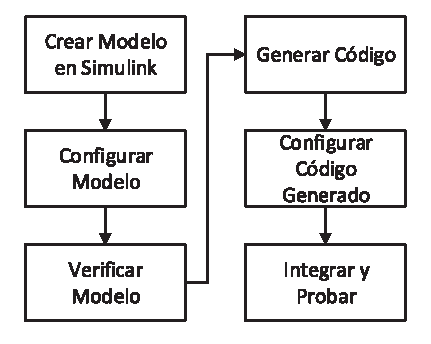
\includegraphics[width=0.5\textwidth]{fig/teorico/Flujo de trabajo simulink coder.pdf}
    \caption{Flujo de trabajo Simulink Coder}
    \label{fig:Simulink_coder_workflow}
\end{figure}

Como se pudo observar en la Figura \ref{fig:Simulink_coder_workflow}, primeramente se debe de diseñar el modelo utilizando bloques de Simulink para representar el sistema o algoritmo a implementar, una vez generado el diagrama se deben de ajustar las configuraciones del modelo, incluyendo parámetros como el tipo de solución, la frecuencia de muestreo y las opciones de simulación, además de esto se deben de realizar simulaciones para verificar que el modelo funcione correctamente y cumpla con los requisitos especificados. 

Finalmente se debe de hacer uso de la herramienta Simulink Coder para generar automáticamente código C o C++ a partir del modelo validado. Adicionalmente a este código generado se pueden realizar configuraciones según se desea su ejecución, estas configuraciones son opciones adicionales para la generación del código, como optimización y estilo de codificación. Una vez aplicados todos los cambios necesarios se debe integrar el código generado en un entorno de desarrollo adecuado y realizar pruebas para asegurar que el código se comporta como se espera en el hardware objetivo.

\section{Código embebido}

El código embebido se refiere a un tipo de software diseñado para operar en dispositivos con recursos limitados, como microcontroladores y sistemas embebidos. 
Este código es fundamental en la programación de dispositivos electrónicos, permitiendo que estos realicen tareas específicas, como gestionar un sistema de 
automatización industrial o incluso operar en dispositivos móviles. Se caracteriza por su ejecución en dispositivos con recursos limitados, su capacidad 
para controlar dispositivos electrónicos, el uso de lenguajes de bajo nivel, la optimización de recursos y la necesidad de garantizar tiempos de respuesta 
determinísticos.

\section{Compilación Cruzada}

La compilación cruzada es un proceso clave en el desarrollo de software que permite compilar código fuente en un sistema operativo o arquitectura de hardware diferente al utilizado para el desarrollo. Este método es especialmente valioso en entornos como sistemas embebidos, donde la plataforma de destino no es adecuada para la compilación directa. Utiliza compiladores específicos, conocidos como compiladores cruzados, que generan código ejecutable para la plataforma de destino desde una plataforma de origen. Esto permite a los desarrolladores trabajar en sus máquinas locales, como Windows o Linux, mientras crean aplicaciones para dispositivos como microcontroladores o sistemas operativos variados.


Además de su uso en sistemas embebidos, la compilación cruzada es fundamental para el desarrollo multiplataforma, ya que facilita la creación de aplicaciones que funcionan en diferentes sistemas operativos sin necesidad de modificar el código base. Este enfoque no solo mejora la eficiencia del proceso de desarrollo y pruebas, sino que también evita la constante transferencia de código a la plataforma de destino. En resumen, la compilación cruzada es una técnica esencial en el desarrollo moderno de software, permitiendo a los desarrolladores abordar múltiples plataformas y arquitecturas con mayor facilidad.

\begin{figure}[h!]
    \centering
    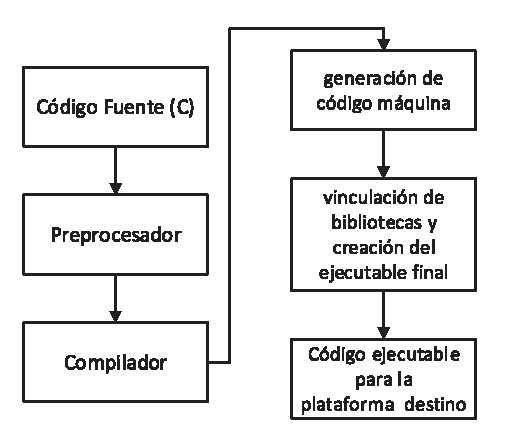
\includegraphics[width=0.5\textwidth]{fig/teorico/Flujo de trabajo xcompiler.pdf}
    \caption{Diagrama de compilación cruzada}
    \label{fig:xcompile_workflow}
\end{figure}

Como se pudo observar en la Figura \ref{fig:xcompile_workflow}, el proceso de compilación de un programa en lenguaje C comienza con el código fuente, que es el conjunto de instrucciones escritas por el programador. A continuación, se utiliza el preprocesador, que lleva a cabo tareas esenciales como la inclusión de archivos y la expansión de macros, generando un archivo intermedio que está listo para ser compilado. Posteriormente, el compilador analiza este archivo intermedio y produce código objeto, una representación en lenguaje máquina que aún no está completamente vinculada. Este código objeto es luego procesado por el ensamblador, que lo convierte en código máquina, específico para la arquitectura del sistema objetivo.

\section{Contenedores}\label{sec:containers}

Docker ha revolucionado la forma en que se desarrollan y despliegan aplicaciones al ofrecer un entorno portátil y consistente. Gracias a su capacidad de empaquetar aplicaciones junto con todas sus dependencias, los desarrolladores pueden estar seguros de que su software funcionará de manera idéntica en cualquier entorno, ya sea local, en la nube o en producción. Esta portabilidad no solo ahorra tiempo en la configuración del entorno, sino que también reduce significativamente los problemas relacionados con "funciona en mi máquina". Además, el aislamiento que proporcionan los contenedores asegura que las aplicaciones operen sin interferencias, lo que es crucial para mantener la estabilidad y el rendimiento.

Por otro lado, la eficiencia de Docker es notable. A diferencia de las máquinas virtuales, los contenedores comparten el núcleo del sistema operativo, lo que permite un uso más optimizado de los recursos y un inicio casi instantáneo. Esto se traduce en una mayor agilidad y rapidez al escalar aplicaciones, ya que se pueden crear y gestionar múltiples instancias de contenedores con facilidad. La capacidad de versionar imágenes también es un gran beneficio, ya que permite a los equipos mantener un historial claro de cambios y revertir a versiones anteriores cuando sea necesario. En conjunto, estas características hacen de Docker una herramienta indispensable para la integración y entrega continua (CI/CD), mejorando significativamente los flujos de trabajo de desarrollo y despliegue.

\section{Protocolos de Comunicación}\label{sec:protocolos_de_comunicacion}

Los protocolos de comunicación son un conjunto de reglas y convenciones que permiten la transmisión de datos entre dispositivos en una red. Estos protocolos son esenciales para garantizar que los dispositivos puedan intercambiar información de manera efectiva y segura \cite{Eterovic2018AnlisisDP}.

\subsection{UART}

El Universal Asynchronous Receiver-Transmitter, por sus siglas en ingles (UART) es un protocolo de comunicación serial ampliamente utilizado para la transmisión de datos entre dispositivos. Su característica principal es que es asíncrono, lo que significa que no requiere una señal de reloj compartida entre el transmisor y el receptor.

\textbf{Características:}

\begin{itemize}
    \item Transmisión Asíncrona: No necesita sincronización de reloj, lo que simplifica su implementación y reduce la complejidad del sistema.
    \item Configuración Simple: Opera comúnmente con configuraciones de 8 bits de datos, 1 bit de parada y 1 bit de paridad opcional, facilitando su uso en diversas aplicaciones.
    \item Distancia de Comunicación: Es efectivo para distancias cortas, generalmente menos de 15 metros, debido a la posible degradación de la señal a medida que aumenta la distancia.
    \item Velocidad de Transmisión: Las tasas de baudios (baud rate) pueden variar desde 300 hasta 115200 bps o más, dependiendo del hardware y las condiciones del entorno.
\end{itemize}

\textbf{Aplicaciones:}

\begin{itemize}
    \item Comunicación entre microcontroladores.
    \item Interfaces para sensores y dispositivos periféricos.
    \item Envío de datos a través de puertos serie en computadoras y dispositivos embebidos.
\end{itemize}

\subsection{SSH}

El Secure Shell (SSH) es un protocolo de red que permite la administración segura de dispositivos y la transferencia de datos a través de redes inseguras. SSH proporciona autenticación y cifrado, garantizando que los datos transmitidos estén protegidos contra ataques maliciosos.

\textbf{Características:}

\begin{itemize}
    \item Cifrado: Utiliza algoritmos de cifrado robustos, como AES, para proteger la información durante su transmisión.
    \item Autenticación: Permite autenticación mediante contraseña o claves públicas, aumentando significativamente la seguridad en el acceso a los sistemas.
    \item Túneles Seguros: Facilita la creación de túneles seguros para otros protocolos, lo que permite la transferencia protegida de datos sensibles.
    \item Interfaz de Línea de Comando: Proporciona acceso remoto a la línea de comandos, permitiendo a los administradores gestionar sistemas sin necesidad de estar físicamente presentes.
\end{itemize}

\section{Computadoras de guía, navegación y control}

Las computadoras de guía, navegación y control son esenciales en diversas aplicaciones, particularmente en aviación, navegación marítima y vehículos autónomos. Su función principal radica en procesar datos de sensores para ofrecer información precisa que facilite la toma de decisiones en tiempo real. Estas tecnologías son fundamentales para garantizar la seguridad y eficiencia en el transporte moderno.

Existen tres tipos principales de computadoras en este ámbito: las computadoras de navegación, que determinan la posición y rumbo de embarcaciones o aeronaves mediante sistemas GPS e inerciales; las computadoras de control, que regulan el movimiento y estabilidad de los vehículos, como los controladores de vuelo; y las computadoras de guía, que ofrecen rutas óptimas a través de sistemas de navegación por satélite. Los componentes clave incluyen sensores que recogen datos del entorno, procesadores que realizan cálculos complejos y interfaces de usuario que permiten la interacción con el sistema.

Las aplicaciones de estas computadoras son variadas y críticas. En la aviación, se utilizan para el control de vuelo en aeronaves comerciales y militares. En la navegación marítima, aseguran rutas seguras para barcos. Además, son integradas en vehículos autónomos como coches y drones, permitiendo una navegación eficiente sin intervención humana. En conjunto, estas tecnologías no solo mejoran la seguridad, sino que también optimizan la eficacia del transporte actual.

\subsection{EXA ICEPS}\label{sec:exaiceps}
La computadora de vuelo EXA ICEPS (Integrated Control and Engine Performance System) es una tecnología avanzada diseñada para gestionar y optimizar el rendimiento del motor y otros sistemas críticos en aeronaves. Su integración de sistemas permite combinar el control del motor con diferentes funciones de la aeronave, lo que resulta en una gestión más eficiente y segura durante el vuelo.

Entre sus principales características se destacan el monitoreo en tiempo real, que proporciona datos sobre el rendimiento del motor, permitiendo a los pilotos tomar decisiones informadas. Además, la EXA ICEPS optimiza el rendimiento al maximizar la eficiencia del combustible y reducir las emisiones, contribuyendo así a operaciones más sostenibles. Sus funciones incluyen el control automático de los parámetros del motor y la facilitación del diagnóstico y mantenimiento predictivo, lo que ayuda a reducir costos operativos.

Este sistema ejemplifica cómo la tecnología moderna está revolucionando la aviación, mejorando tanto la seguridad como la eficiencia operativa. Al integrar múltiples funciones y proporcionar información crítica en tiempo real, la EXA ICEPS no solo optimiza el rendimiento de las aeronaves, sino que también promueve prácticas más sostenibles en la industria.
\section{Revisión literaria}
En los últimos años, las computadoras de guía, navegación y control han mostrado grandes avances en el desarrollo de sistemas autónomos.

\subsection{Desarrollo de sistemas de navegación}

En 2022, se presentó un sistema de planificación y control de navegación para vehículos autónomos en entornos urbanos. Este sistema permite la planificación 
de rutas basadas en la posición actual del vehículo y su destino, utilizando un controlador clásico que asegura el seguimiento de la trayectoria mediante 
odometría y correcciones visuales. Los resultados se simularon utilizando herramientas como ROS y Gazebo, lo que demuestra la viabilidad de estos sistemas en 
entornos complejos \cite{BarreraRamrez2022SistemaDP}. 

\subsection{Transformación de Lenguaje de Bloques a Código C}

La traducción de código de control de lenguaje de bloques a C implica un proceso de conversión donde cada bloque visual se asocia con una estructura de código 
en C. Esto se puede hacer utilizando herramientas de software que generan automáticamente el código C a partir de la lógica definida en el entorno de bloques. 
Este proceso no solo facilita la programación, sino que también permite la optimización del código generado para mejorar el rendimiento en sistemas de navegación 
autónoma.

\subsubsection{XOD}

XOD es un entorno de programación visual basado en bloques que permite a los usuarios crear programas para microcontroladores como Arduino. Este software 
genera automáticamente código en C++ a partir de la lógica definida en bloques. Los usuarios pueden conectar componentes gráficamente y, al finalizar, acceder 
al código generado, que es abierto y personalizable. XOD es gratuito y permite la creación de nuevos nodos para componentes específicos, lo que facilita la 
adaptación a diferentes proyectos \cite{Snchez2020ProgramacinDL}.

\subsubsection{Visual Microcontroller}
Este software proporciona un lenguaje de programación gráfico para microcontroladores, desarrollado en C\#. Utiliza una interfaz gráfica que permite a los 
usuarios diseñar diagramas que representan la lógica de control. El sistema compila el código a partir de diagramas gráficos, generando código intermedio 
en C antes de llegar al código hexadecimal necesario para la programación del microcontrolador \cite{Sacta2011DesarrolloDU}.


\subsubsection{LabVIEW}

LabVIEW es un entorno de desarrollo que utiliza un enfoque gráfico para la programación. Aunque es más conocido en el ámbito de la ingeniería, también 
permite la generación de código en C. LabVIEW facilita la creación de aplicaciones de control y adquisición de datos, y su capacidad para traducir 
diagramas de bloques a código C lo convierte en una opción útil para proyectos que requieren un control preciso de hardware.

\subsubsection{Simulink}
Como se mencionó anteriormente, Simulink, parte de MATLAB, proporciona un entorno gráfico para modelar, simular y analizar sistemas dinámicos. 
Permite a los usuarios crear modelos utilizando bloques y, posteriormente, generar código C automáticamente a partir de estos modelos. Esta 
herramienta es especialmente valiosa en aplicaciones de ingeniería donde se requiere un alto grado de precisión y control sobre el 
comportamiento del sistema.

\section{Avances recientes en GNCs }

En el marco del proyecto EROSS+ (European Robotic Orbital Support Services), se ha trabajado en el diseño de un sistema GNC altamente autónomo 
para misiones de servicio robótico en órbita. Este proyecto, que abarca desde 2021 hasta 2023, busca integrar técnicas avanzadas de navegación 
visual y control de cumplimiento para la captura y manipulación de satélites, mostrando un enfoque en la autonomía y la eficiencia operativa \cite{Casu2023EROSSPA}.

Otro desarrollo notable es el programa de NASA sobre GNC autónomo, que incluye sistemas para el transbordador espacial. Este programa se centra en la optimización 
de trayectorias de vuelo y la adaptación de sistemas GNC para diferentes condiciones de vuelo, lo que demuestra la importancia de la flexibilidad en el diseño de 
estos sistemas \cite{Bordano1991AutonomousGN}.

Además, la actividad VV4RTOS, apoyada por la Agencia Espacial Europea, se ha centrado en la verificación y validación de sistemas de control basados en optimización. 
Esto incluye el desarrollo de software GNC en tiempo real, lo que permite una validación más efectiva y segura de los sistemas diseñados \cite{Loureno2023VerificationV}.

\subsection{Programación de Sistemas GNC}
Los lenguajes de bloques, como Simulink, son comúnmente utilizados para diseñar y simular sistemas de control. Estos lenguajes permiten a los ingenieros visualizar 
el flujo de datos y las interacciones entre componentes de manera intuitiva. Sin embargo, la necesidad de traducir estos modelos a código C es crucial para su 
implementación en hardware real.

A pesar de los avances, existen desafíos significativos en la implementación de sistemas GNC. La variabilidad en los entornos operativos y la necesidad de adaptarse 
a condiciones cambiantes requieren algoritmos robustos y adaptativos. La optimización de estos sistemas es fundamental para asegurar su efectividad en misiones 
críticas.

Un estudio reciente sobre el sistema CubeNav destaca la importancia de desarrollar herramientas de análisis de navegación que faciliten las operaciones de GNC 
en misiones de CubeSats. Este enfoque busca reducir la curva de aprendizaje y minimizar errores humanos, lo que es esencial para misiones de bajo presupuesto 
y alta complejidad \cite{Loureno2023VerificationV}.
  \chapter{Tarjeta de desarrollo}
\label{ch:especifico1}

En este capítulo se pretende identificar una plataforma de hardware para el desarrollo de un modelo de ingeniería de
una computadora de guía, navegación y control espacial por sus siglas en ingles (GNC), para llevar a cabo este objetivo 
se plantean los requerimientos que se deben de tomar en cuenta para elegir una tarjeta de desarrollo que logre satisfacer
las necesidades de este proyecto, seguido de esto se seleccionaran un grupo de tarjetas las cuales cumplan con los 
requerimientos previamente establecidos, estas serán comparadas para poder determinar cuál de las tarjetas de desarrollo 
seleccionadas puede cumplir de mejor forma la tarea seleccionada.

\section{Selección de la tarjeta de desarrollo}
    Para la selección de la tarjeta de desarrollo se partirá de la definición de los requerimientos de operación del sistema, 
    esto tomando en cuenta las operaciones más comunes que realizan los sistemas GNC, una vez definidos los requerimientos, se 
    seleccionaran al menos 3 tarjetas candidatas, esto con el fin de establecer los criterios de comparación para el desarrollo
    de una matriz de Pugh.

\subsection{Requerimientos de la aplicación}

Al elegir una tarjeta de desarrollo para un sistema de guía, navegación y control (GNC) en aplicaciones espaciales, 
se deben de tener en cuenta varios factores clave. Dentro de ellos se encuentran el procesamiento, mas precisamente
la capacidad de calculo, ya que estos sistemas reuqieren de un procesamiento intensivo para los calculos de trayectoria
, estimacion de estado y control. Seguido de esto se debe de considerar que sea un sistema de baja latencia, ademas que
el mismo tenga soporte para sensores y actuadores para poder mediir y controlar el sistema, ademas de esto los puertos
de entrada y salida deben ofrecer la presicion necesaria ara leer los datos de los sensores que se conecten al mismo.

Por otro lado el sistema debe de contener capacidades de tiempo real estricto ya que los sistemas GNC deben de tomar
desiciones criticas en el momento requerido. ademas de tener la capacidad de ejecutar un sistema opereativo de tiempo real
(RTOS) o bien Linux en tiempo real. Tambien un aspecto importante a contener por la tarjeta de desarrollo es el consumo de
energia, esto sin dejar de lado las capacidades de simulacion y pruebas, ya que, en la interfaz de simulacion la tarjeta se
debe de poder conectar a un entorno de pruebas de hardware-in-the-loop por sus siglas en ingles (HIL), ademas de las
capacidades de depuracion y monitoreo.

Finalmente se deben de tomar en cuenta aspectos como lo son el Tamanno, peso y forma de la trjeta buscando que las mismas contengan 
un tamanno compacto ya que los sistemas espaciales siempre se deben de integrar en espacios reducidos y la resistencia del mismo.

\subsection{Tarjetas candidatas}
Bajo los requerimientos planteados anteriomente se eligieron las siguientes tarjetas de desarrollo, las mismas se presentaran con sus
caracteristicas.

\subsubsection{Xilinx ZCU102 Evaluation Kit}

La tarjeta de desarrollo ZCU102 contiene procesamiento basado en Zynq UltraScale+ MPSoC, el cual combina un procesador ARM Cortex-A53 de 
64 bits con una FPGA de alto rendimiento, la cual es excelente para el procesamiento en tiempo real y algorimos personalizados.

Por otro aldo esta ofrece una amplia gama de interfaces de comunicacion como: PCIe, Ethernet, I2C, SPI, UART, GPIO. En cuanto a la eficiencia energetica esta opcion contiene mecanismos para el control de energia, ademas de ser compatible con entornos de 
de simulacion y tiene interfaces JTAG oara una buena depuracion. finalmente es una tarjeta ampliamente utilizada en la industria en Sistemasd
de prototipos avanzados y despliegue de HIL.

En sintesis esta opcion ofrece un procesamiento potente y versatil ademas de ser excelente para desarrollar y escalar sistemas GNC complejos, 
por otro lado es una tarjeta de desarrollo costosa.

\subsubsection{NVIDIA Jetson AGX Xavier}

Para el caso de la tarjeta AGX Xavier de NVIDIA incorpora una CPU ARM v8.2 de 64 bits y una GPU NVIDIA Volta, prestaciones las cuales se encargan de proporcionar
un alto nivel de procesamiento de datos en paralelo especualmente utilizado para aplicaciones de vision por computador o inteligencia artificial para sistemas GNC. 

Las interfases de comunicacion presentes en esta tarjeta son puertos I2C, SPIm UART y GPIO ademas de contener adicionalmente soporte nativo para camaras y sensores de
alta gama. Ademas presenta capacidades en tiempo real ya que se puede implementar con el NVIDIA Jetpack SDK. 

En cuanto a la eficiencia energetica, la misma posee un diseno optimizado para bajo consumo. ademas de ser compatible con interfases de pruebas y simulacion mediante el 
uso de entornos como Tensor RT y otras plataformas propietarias del desarrollador de la tarjeta de desarrollo.

Esta tarjeta es ideal para sistemas GNC con un procesamiento intensivo de datos ya sean de vision por computador o bien inteligencia artificial, por otro lado posee un desarrollo potente 
para el procesamiento de tares en paralelo o bien de aprendizaje reforzado, finalmente contiene un buen soporte para aplicaciones en tiempo real y simulaciones. Por otro lado contiene un 
bajo procesamiento logico comparado con las FPGA para aplicaciones en tiempo real extremo, y esta tarjeta de desarrollo se encuentra mas enfocada en el la implementacion de soluciones que
requieran inteligencia artificial.

\subsubsection{TMS320C6678 Development Kit}

La tarjeta TMS320C6678 es basada en un procesador para procesamiento digital de senales (DSP) de 8 nucleos, esta enfocado a aplicaciones de procesamiento intensivo en tiempo real, soporta
interfases como lo son Ethernet, SPI, UARTm I2C y GPIO, ademas de tener opciones para expandir la conectividad de la misma, por otro lado como mencionamos anteriormente es uno de los sistemas
mas optimizados para el procesamiento en tiempo real por medio de la plataforma propietaria TI RTOS.

Sobre la eficiencia energetica, esta tarjeta de desarrollo ofrece herramientas especificas para la optimizacion del consumo de energia, hacinedola adecuada para entornos de consumo energetico 
restringido, finalmente es compatible con Code Composer Studio, el cual es un entorno de desarrollo integrado que facilita las labores de integracion, simulacion y depuracion. Por tanto podemos
decir que es una tarjeta de desarrollo muy adecuada para los sistemas de procesamiento de senañes y control, tiene una gran capacidad para soportar aplicaciones industriarles y aeroespaciales. Por otro
lado, podemos ver que es un plataforma menos flexible que una FPGA. 

\subsubsection{ZedBoard de Avnet}

Para la tarjeta ZedBoard en cuanto a procesamiento tenemos que utiliza un procesador Xilinx Zynq-7000 APSoC el cual combina un procesador ARM Cortex-A9 dual core con una FPGA programable, de esta froma 
tomando el procesador ARM el cual es ideal para ejecutar algoritmos de control y  logica de navegacion en un entrno de RTOS o bien Linux, por otro lado la FPGA Zynq-7000 permite la ejecucion de tareas 
de procesamiento paralelo en hardware como el filtrado de sennales o algoritmos de estimacion de estad, ofreciendo baja latencia y flexibilidad en tiempo real.

En cuanto a las interfases de entrada y salida, incluye varias opciones como lo son: GPIO, I2C, SPI, UART. Ademas de esto contiene puertos Ethernet, micro usb y HDMI los cuales resultan utiles para la 
comunicacion externa y visualizacion de los sistemas de desarrollo.

La combinacion de un procesador ARM con una FPGA permite un equilibrio en el consumo de energia ya que la mayoria de tareas intensivas se pueden llevar a cabo en la FPGA y el SoC Zynq ofrece opciones de 
ahorro de energia lo cual siempre representa un beneficio para las aplicaciones embebidas. En cuanto a la pruebas y simulaciones cuenta con entornos como vivado y SDK de Xilinx esto con el fin de realizar
simulaciones de HIL. Por otro lado ofrece aplicaciones para depuracion como lo es Jtag para el monitoreo en tiempo real de las aplicaciones ejecutandose en la FPGA y en el procesador ARM.
\subsection{Criterios de comparación}

Una vez presentadas las terjetas de desarrollo candidatas se procede con la definicion de los criterios de comparacion: para este caso los criterios a tomar en cuenta son los siguientes:

\begin{enumerate}
    \item Capacidad de procesamiento: La capacidad de procesamiento en dispositivos de desarrollo para sistemas GNC es crucial porque garantiza la ejecución en tiempo real de algoritmos complejos, como los de control y fusión de sensores, que son esenciales para la estabilidad y precisión del sistema. Permite procesar grandes volúmenes de datos de múltiples sensores de manera simultánea y rápida, ejecutar tareas en paralelo, y realizar cálculos intensivos como la planificación de trayectorias y control adaptativo. Además, un procesamiento robusto facilita la simulación HIL, asegurando pruebas y simulaciones realistas.

    \item Soporte para sensores y actuadores: El soporte para sensores y actuadores es esencial en dispositivos de desarrollo para sistemas GNC porque estos sistemas dependen de la entrada de múltiples sensores como acelerómetros, giroscopios, GPs, entre otros, para monitorear y estimar la posición, orientación y velocidad del vehículo en tiempo real. La capacidad de interactuar directamente con estos sensores, y con actuadores que ejecutan las acciones de control, es fundamental para garantizar la retroalimentación continua y precisa necesaria para el correcto funcionamiento del sistema GNC. Interfaces como I2C, SPI, UART, y GPIO permiten esta integración, asegurando un control eficiente y adaptable.

    \item Capacidad de trabajo en tiempo real: La capacidad de trabajo en tiempo real es vital en dispositivos de desarrollo para sistemas de guía, navegación y control (GNC) porque estos sistemas requieren respuestas inmediatas y precisas ante cambios en el entorno o en las condiciones del vehículo. Los algoritmos de control, como los de estabilidad y trayectoria, deben ejecutarse sin demoras para garantizar la seguridad y el rendimiento óptimo del sistema. Sin procesamiento en tiempo real, las decisiones de control podrían retrasarse, afectando la estabilidad y el control del vehículo, lo cual es crítico en aplicaciones como navegación autónoma o vuelo espacial.

    \item Consumo de energia: El consumo de energía es crucial en dispositivos de desarrollo para sistemas de guía, navegación y control (GNC), especialmente en aplicaciones espaciales o autónomas, donde los recursos energéticos son limitados. Un consumo eficiente permite que el sistema funcione de manera prolongada sin comprometer su rendimiento, maximizando la duración de la misión y asegurando que los componentes críticos, como sensores y actuadores, siempre reciban suficiente energía. Además, la gestión adecuada del consumo evita el sobrecalentamiento y prolonga la vida útil de los dispositivos, lo que es fundamental en entornos de operación prolongada o difíciles de acceder.

    \item Caracteristicas Fisicas: Las características físicas, como el tamaño, peso y forma, son importantes en dispositivos de desarrollo para sistemas de guía, navegación y control (GNC) porque estos sistemas suelen implementarse en entornos con restricciones de espacio y peso, como en vehículos aéreos, drones o satélites. Un dispositivo compacto y ligero facilita la integración en estos sistemas sin afectar su desempeño ni su capacidad de carga. Además, un diseño físico optimizado es clave para minimizar los efectos de vibraciones, choques o cambios de temperatura, asegurando un funcionamiento fiable en condiciones extremas.

    \item Costo: El costo es un factor importante en dispositivos de desarrollo para sistemas de guía, navegación y control (GNC) porque influye directamente en la viabilidad económica del proyecto, especialmente en fases de prototipado o prueba. Un dispositivo con un costo adecuado permite realizar iteraciones y pruebas sin superar el presupuesto, facilitando el acceso a tecnologías avanzadas sin comprometer la calidad. Además, un costo equilibrado permite escalar el proyecto o implementar múltiples sistemas de prueba, optimizando el desarrollo sin sacrificar funcionalidad o capacidad técnica.

    \item Escalabilidad del sistema: 
    La escalabilidad del sistema es crucial en dispositivos de desarrollo para sistemas de guía, navegación y control (GNC) porque permite adaptar el hardware y software a medida que el proyecto crece en complejidad o requisitos técnicos. Un dispositivo escalable facilita la integración de nuevos sensores, algoritmos más avanzados o mayores capacidades de procesamiento sin necesidad de cambiar completamente la plataforma. Esto ahorra tiempo y costos, además de asegurar que el sistema pueda evolucionar para cumplir con las demandas de futuras fases del desarrollo o nuevas aplicaciones, manteniendo la flexibilidad y la eficiencia.

\end{enumerate}
\newpage

\section{Matriz de Pugh}

% Please add the following required packages to your document preamble:
% \usepackage{graphicx}
\begin{table}[h!]
    \centering
    \caption{Matriz de Pugh para seleccionar la tarjeta de desarrollo que mejor de adapte a los requerimientos del proyecto}
    \label{tab:Pug_tarjetas_desarrollo}
    \resizebox{\columnwidth}{!}{%
    \begin{tabular}{lccccc}
    \hline
    \multicolumn{1}{|l|}{Criterios} & \multicolumn{1}{l|}{Peso} & \multicolumn{1}{l|}{ZCU102} & \multicolumn{1}{l|}{AGX Xavier} & \multicolumn{1}{l|}{TMS320C6678} & \multicolumn{1}{l|}{Zedboard} \\ \hline
    \multicolumn{1}{|l|}{Capacidad de   procesamiento} & \multicolumn{1}{c|}{15} & \multicolumn{1}{c|}{15} & \multicolumn{1}{c|}{15} & \multicolumn{1}{c|}{8} & \multicolumn{1}{c|}{10} \\ \hline
    \multicolumn{1}{|l|}{Soporte para   sensores} & \multicolumn{1}{c|}{15} & \multicolumn{1}{c|}{15} & \multicolumn{1}{c|}{15} & \multicolumn{1}{c|}{15} & \multicolumn{1}{c|}{15} \\ \hline
    \multicolumn{1}{|l|}{Soporte para   actuadores} & \multicolumn{1}{c|}{15} & \multicolumn{1}{c|}{15} & \multicolumn{1}{c|}{15} & \multicolumn{1}{c|}{15} & \multicolumn{1}{c|}{15} \\ \hline
    \multicolumn{1}{|l|}{Soporte de   sistemas de tiempo real} & \multicolumn{1}{c|}{20} & \multicolumn{1}{c|}{20} & \multicolumn{1}{c|}{20} & \multicolumn{1}{c|}{15} & \multicolumn{1}{c|}{20} \\ \hline
    \multicolumn{1}{|l|}{Caracteristicas   Fisicas} & \multicolumn{1}{c|}{10} & \multicolumn{1}{c|}{4} & \multicolumn{1}{c|}{7} & \multicolumn{1}{c|}{10} & \multicolumn{1}{c|}{10} \\ \hline
    \multicolumn{1}{|l|}{Costo de la   tarjeta} & \multicolumn{1}{c|}{15} & \multicolumn{1}{c|}{7} & \multicolumn{1}{c|}{10} & \multicolumn{1}{c|}{10} & \multicolumn{1}{c|}{15} \\ \hline
    \multicolumn{1}{|l|}{Escalabilidad   del sistema} & \multicolumn{1}{c|}{10} & \multicolumn{1}{c|}{10} & \multicolumn{1}{c|}{6} & \multicolumn{1}{c|}{6} & \multicolumn{1}{c|}{10} \\ \hline
     & \multicolumn{1}{l}{} & \multicolumn{1}{l}{} & \multicolumn{1}{l}{} & \multicolumn{1}{l}{} & \multicolumn{1}{l}{} \\ \cline{1-1} \cline{3-6} 
    \multicolumn{1}{|l|}{Suma general} & \multicolumn{1}{l|}{} & \multicolumn{1}{c|}{86} & \multicolumn{1}{c|}{88} & \multicolumn{1}{c|}{79} & \multicolumn{1}{c|}{95} \\ \cline{1-1} \cline{3-6} 
    \multicolumn{1}{|l|}{Posicion} & \multicolumn{1}{l|}{} & \multicolumn{1}{c|}{3} & \multicolumn{1}{c|}{2} & \multicolumn{1}{c|}{4} & \multicolumn{1}{c|}{1} \\ \cline{1-1} \cline{3-6} 
    \end{tabular}%
    }
    \end{table}

    Como se pudo observar en la Tabla \ref{tab:Pug_tarjetas_desarrollo}, un claro ganador segun los requerimientos establecidos para este proyecto ha sido la tarjeta de desarrollo zedbaord ya que es la mejor opcion en cuanto a caracteristicas como lo son la capacidad de procesamiento y \dots

\section{Plataforma seleccionada}

Como se pudo observar en la Tabla \ref{tab:Pug_tarjetas_desarrollo}, la tarjeta de desarrollo seleccionada fue la Trajeta Zedboard de Avnet. La ZedBoard es una tarjeta de desarrollo basada en el SoC (System-on-Chip) Xilinx Zynq-7000. Diseñada para aplicaciones de desarrollo en sistemas embebidos y de procesamiento de señales, la ZedBoard combina la potencia de un procesador ARM con la flexibilidad de una FPGA (Field Programmable Gate Array), proporcionando una plataforma versátil para la investigación, el desarrollo y la prueba de diversas aplicaciones, incluidas las de guía, navegación y control (GNC).

\subsection{Especificaciones principales}

Como se meciono en el capitulo \ref{ch:marco} en la Tabla \ref{tab:zedboard} y anteriormente en este capitulo la tarjeta en cuestion presenta las siguientes especificaciones principales.

\subsubsection{Procesador y FPGA}
SoC Xilinx Zynq-7000: La ZedBoard integra un procesador ARM Cortex-A9 dual-core junto con una FPGA programable de la serie 7-Series.
ARM Cortex-A9: Ofrece un rendimiento de procesamiento general que puede ejecutar sistemas operativos como Linux o FreeRTOS, lo que es útil para tareas de control y procesamiento de datos.
FPGA: La FPGA proporciona capacidad para implementar lógica personalizada, lo que permite el desarrollo de algoritmos específicos en hardware para procesamiento en tiempo real y alta velocidad.
\subsubsection{Interfaces de E/S}
GPIO: General Purpose Input/Output, permite la interacción con una amplia gama de periféricos y sensores.
I2C, SPI, UART: Protocolos de comunicación estándar que facilitan la integración con diversos dispositivos de sensor y actuadores.
Ethernet: Conectividad de red para comunicación y transmisión de datos.
USB: Puertos USB para conexión de dispositivos externos y almacenamiento.
HDMI: Salida de video para visualización de datos y control gráfico.
JTAG: Para depuración y programación de la FPGA y el procesador ARM.
\subsubsection{Memoria}
RAM: Incluye memoria DDR3 SDRAM para el procesador y la FPGA, proporcionando espacio suficiente para la ejecución de sistemas operativos y algoritmos complejos.
Flash: Memoria flash para almacenamiento de configuraciones y datos persistentes.
\subsubsection{Alimentación y Consumo de Energía}
La ZedBoard se alimenta típicamente a través de una entrada de 5V, con un diseño que optimiza el consumo energético para aplicaciones de desarrollo. Sin embargo, el consumo real depende del uso de la FPGA y el procesador.
\subsubsection{Tamaño y Factor de Forma}
Dimensiones: Aproximadamente 15.24 cm x 22.86 cm (6 x 9 pulgadas), lo que la hace adecuada para prototipos sin ser excesivamente grande.
Diseño: Compacta pero con suficiente espacio para interfaces y módulos adicionales.
\subsubsection{Capacidades de Desarrollo}
Entornos de Desarrollo: Compatible con Xilinx Vivado Design Suite y SDK, proporcionando herramientas avanzadas para diseño, simulación, y depuración.
Ejemplos de Aplicaciones: Adecuada para aplicaciones que requieren procesamiento en paralelo, desarrollo de sistemas embebidos, y prueba de algoritmos de control.

\section{Reflexión final}

Como se pudo observar a lo largo de este capitulo se analizaron los requerimientos de hardware que se deben de tomar en cuenta para el desaarrollo de este proyecto, seguido de esto se tomaron cuatros tarhjetas de desarrolo con el fin de elegir entre las que presentaran las prestaciones adecuadas para la tarea a realizar. Por un lado se tenian tarjetas muy potentes como xxxx y xxxx y por otro lado se tenian tarjetas de grandes dimenciones como la xxx y xxxx. Segun los parametros definidos se elige la tarjeta xxxx con numero de parte xxx para continuar con el desarrollo de este proyecto.
  \chapter{Flujo de trabajo para la implementación de software para GNC embebido}
\label{ch:especifico2}

Como se pudo observar en el capítulo \ref{ch:especifico1}, se realizó la selección de la tarjeta de desarrollo Zedboard para el desarrollo del proyecto, además de esto uno de los parámetros que se tomó en cuenta fue la compatibilidad de esta con el flujo de trabajo de Yocto Project.

Es por esto que en este capítulo se pretenden establecer los flujos de trabajo para el prototipado de algoritmos de control de orientación y navegación para aplicaciones espaciales. Esto mediante el uso de MATLAB Simulink para tomar un caso de estudio como ejemplo.

Una vez seleccionado el caso de estudio se convierte el código por medio de la transformación de modelo de Simulink a un modelo de código C, esto con el objetivo de poder embeber el código C por medio del flujo de trabajo de Yocto Project y finalmente probar el mismo en la tarjeta de desarrollo seleccionada.

De esta forma se puede comparar los resultados obtenidos y el tiempo de ejecución que llevo la tarea en el computador y en el sistema embebido.


\begin{figure}[h!]
    \centering
    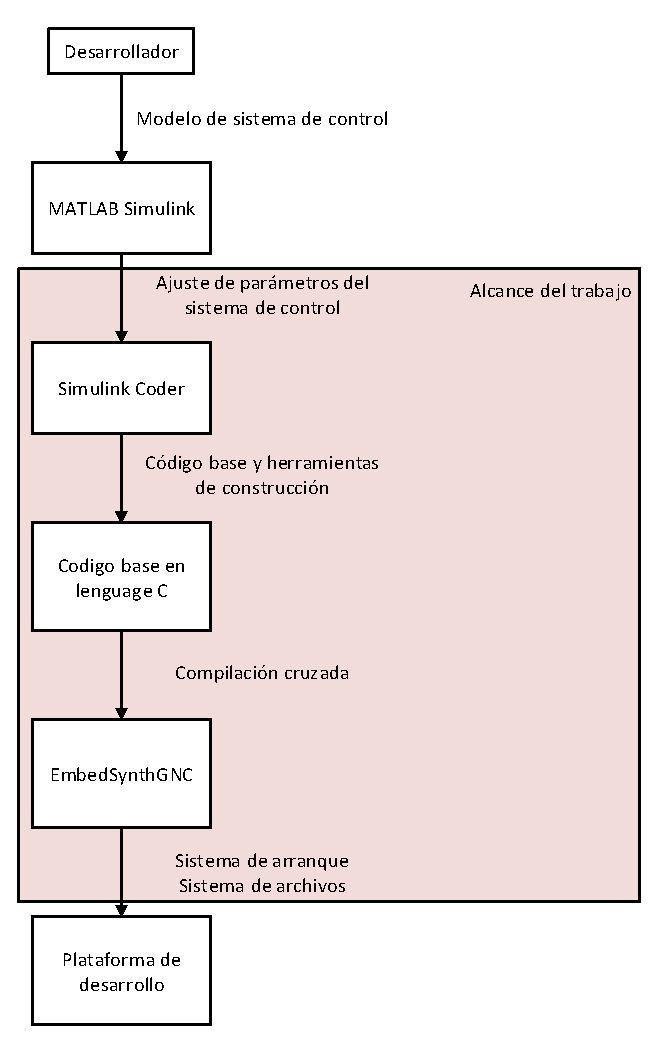
\includegraphics[width=0.3\textwidth]{fig/especifico_2/Diagrama general del proyecto.pdf}
    \caption{Diagrama general del flujo de trabajo propuesto}
    \label{fig:diagrama_flujo_trabajo}
\end{figure}


En la Figura \ref{fig:diagrama_flujo_trabajo}, se muestra un diagrama del flujo de trabajo general. En este capítulo se trabajará en la sección remarcada en rojo la cual engloba la generación del modelo utilizado como caso de estudio, la validación del mismo en MATLAB Simulink, la generación de un código en lenguaje C y la incorporación del mismo en el flujo de trabajo de Yocto Project.

\section{Selección del caso de estudio}

Como caso de estudio se seleccionó una aplicación la cual permitiera una comparación de resultados antes del procesado y después del mismo, es por esto que se decidió implementar un filtro  de tipo paso bajo haciendo uso de los siguientes bloques de MATLAB Simulink. 

\begin{itemize}
    \item Onda seno
    \item Suma
    \item Función de transferencia
    \item Generador de archivo de salida
\end{itemize}

La configuración seleccionada para el primer generador de onda seno es:

\begin{itemize}
    \item Amplitud = 1
    \item Bias = 0 
    \item Frecuencia = 1 rad/s
    \item Fase = 0 
    \item Tiempo de muestreo = 0 
\end{itemize}

Por otro lado, para la segunda onda se tiene la configuración:

\begin{itemize}
    \item Amplitud = 1
    \item Bias = 0 
    \item Frecuencia = 12 rad/s
    \item Fase = 0 
    \item Tiempo de muestreo = 0 
\end{itemize}

Ya que al sumar ondas de diferentes frecuencias, se puede observar un fenómeno llamado modulación, donde la onda resultante presenta un patrón que varía en el tiempo.

\begin{equation}
    y(t) = \sin(t) + \sin(12t)
    \label{eq:funcion_de_suma_de_ondas}
\end{equation}

Por otro lado la función de transferencia a utilizar en el filtro será:

\begin{equation}
    H(S) = \frac{1}{S+1}
    \label{eq:funcion_de_transferencia_filtro}
\end{equation}

Al aplicar el filtro a la señal compuesta,  la onda $\sin(t)$ pasará a través del filtro con poca atenuación, mientras que la onda $\sin(12t)$ será significativamente atenuada debido a su  alta frecuencia.

\begin{figure}[h!]
    \centering
    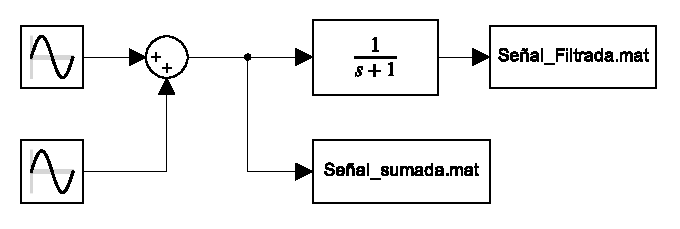
\includegraphics[width=0.5\textwidth]{fig/especifico_2/Diagrama matlab simulink.pdf}
    \caption{Diagrama MATLAB Simulink}
    \label{fig:diagrama_matlab_simulink}
\end{figure}

Estos bloques mencionados anteriormente se colocan como se muestra en la Figura \ref{fig:diagrama_matlab_simulink} de modo que se obtienen como salida del sistema dos archivos, uno llamado señal sumada el cual contiene los datos crudos de la suma de las dos señales y otro denominado señal filtrada el cual contiene los datos de la señal filtrada por la función de transferencia.

\subsection{Simulación del caso de estudio en MATLAB Simulink}\label{subsec:simulacion_caso_de_estudio}

\begin{figure}[h!]
    \centering
    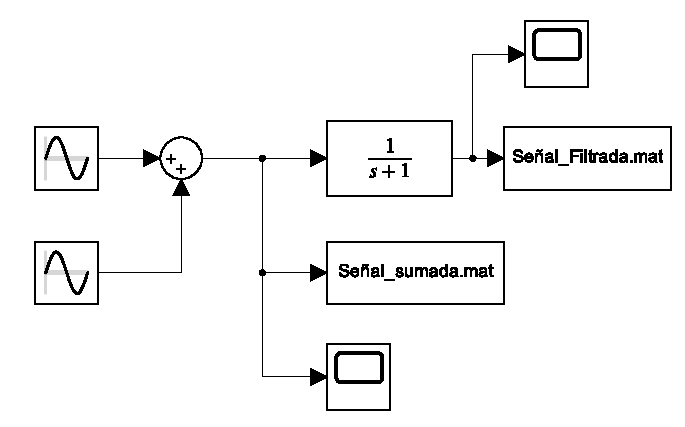
\includegraphics[width=0.5\textwidth]{fig/especifico_2/Diagrama matlab simulink scope.pdf}
    \caption{Diagrama MATLAB Simulink para poder observar las salidas}
    \label{fig:diagrama_matlab_simulink_graficos}
\end{figure}

Utilizando el diagrama de la Figura \ref{fig:diagrama_matlab_simulink}, además de los parámetros configurados anteriormente se colocan dos bloques de gráfico en el diagrama como se muestra en la Figura \ref{fig:diagrama_matlab_simulink_graficos}, esto con el objetivo de poder observar las señales de salida en cada uno de los puntos de interés. 


\begin{figure}[htbp]
    \centering
    \begin{subfigure}[b]{0.45\textwidth}
        \centering
        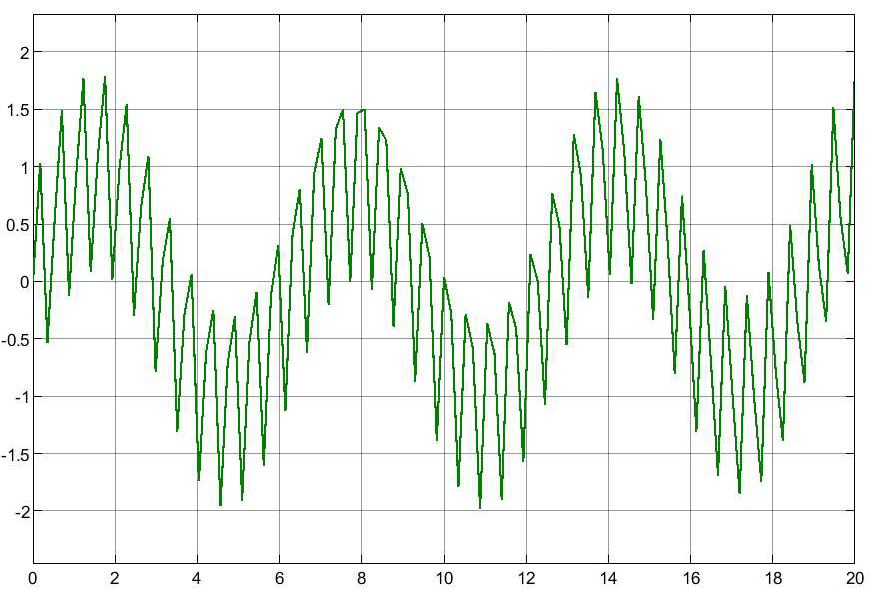
\includegraphics[width=\textwidth]{fig/especifico_2/onda_modulada.pdf}
        \caption{Ondas Moduladas}
        \label{fig:onda_modulada}
    \end{subfigure}
    \hfill
    \begin{subfigure}[b]{0.45\textwidth}
        \centering
        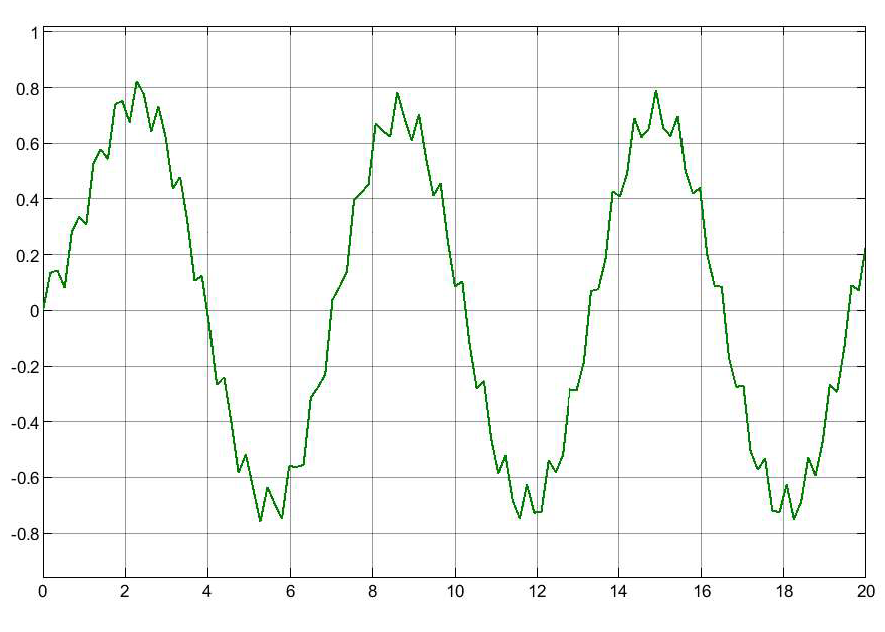
\includegraphics[width=\textwidth]{fig/especifico_2/onda_filtrada.pdf}
        \caption{Onda resultante luego de la función de transferencia}
        \label{fig:onda_filtrada}
    \end{subfigure}
    \caption{Salida resultante del diagrama mostrado en la Figura \ref{fig:diagrama_matlab_simulink_graficos}}
    \label{fig:salida_resultante_diagrama_graficos}
\end{figure}


Como se puede observar en la Figura \ref{fig:onda_modulada} se puede observar la salida de la suma de las dos señales senoidales, por otro lado en la Figura \ref{fig:onda_filtrada} se puede observar la salida de la función de transferencia.

\subsubsection{Resultados obtenidos con la ejecución de la simulación}

Como se mencionó anteriormente los resultados obtenidos se pueden observar en la Figura \ref{fig:salida_resultante_diagrama_graficos}, siendo la salida esperada de la función de transferencia, ya que al ser un filtro paso bajo atenúa las señales que estén por debajo de la frecuencia de corte, que para este filtro es de 1 $rad/s$. Como la señal compuesta contiene una onda seno con frecuencia de 1 $rad/s$ y otra con frecuencia de 12 $rad/s$ es posible observar aun componentes de la frecuencia atenuada.

\section{Flujo de trabajo de la aplicación de transformación de modelo a modelo}

Para poder cumplir con el objetivo de embeber el sistema, se debe de hacer uso del MATLAB Simulink Coder, el cual tiene la capacidad de convertir un sistema de control generado en MATLAB Simulink, en un código C. Algunos de los parámetros que se pueden configurar en este transformador de modelos son: parámetros de la solución, implementación en hardware y generación de código.

A lo largo de este capítulo se definirán los parámetros que se deben de utilizar y el funcionamiento de estos dentro de la generación del código C.

\subsection{Simulink Coder}\label{subsec:simulink_coder}

Una vez comprobado el comportamiento esperado por el caso de estudio se puede proceder con la ejecución del flujo de trabajo de MATLAB Simulink Coder, esto con el fin de transformar el modelo generado en Simulink a un modelo de lenguaje de programación C. Cabe destacar que para esta implementación se utilizó el diagrama que se muestra en la Figura \ref{fig:diagrama_matlab_simulink}, ya que, este solamente contiene como salida los archivos con los datos numéricos del sistema y no contiene las salidas gráficas agregadas en \ref{subsec:simulacion_caso_de_estudio}.


\subsection{Definición de parámetros}

\begin{figure}[h!]
    \centering
    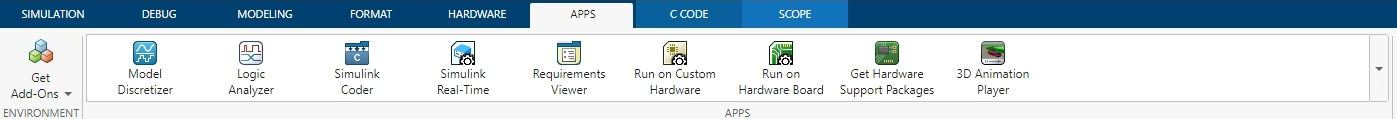
\includegraphics[width=0.8\textwidth]{fig/especifico_2/paso_a_paso_mtmt/apps.png}
    \caption{Pestaña Aplicaciones}
    \label{fig:pestana_apps}
\end{figure}

\begin{figure}[h!]
    \centering
    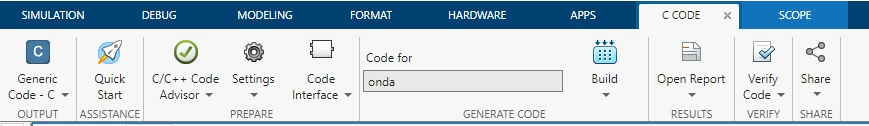
\includegraphics[width=0.8\textwidth]{fig/especifico_2/paso_a_paso_mtmt/c_code.png}
    \caption{Pestaña código C}
    \label{fig:pestana_c_code}
\end{figure}

\begin{figure}[h!]
    \centering
    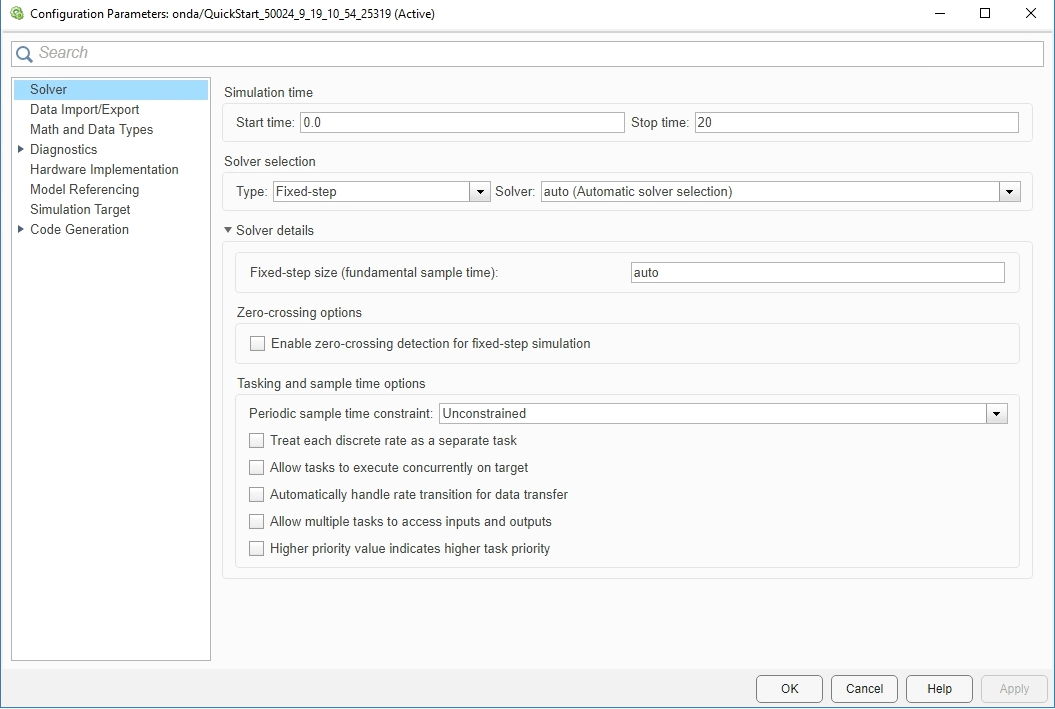
\includegraphics[width=0.8\textwidth]{fig/especifico_2/paso_a_paso_mtmt/configuration_parameters.png}
    \caption{Configuración de parámetros}
    \label{fig:pestana_config}
\end{figure}

Para la definición de parámetros, se debe de estar en el entorno de MATLAB Simulink, una vez en el entorno mencionado anteriormente se debe ir a la pestaña denominada Aplicaciones, o bien APPS como se muestra en la Figura \ref{fig:pestana_apps}, se deberá de seleccionar la aplicación denominada Simulink Coder, cuando seleccionamos esta opción se abrirá una pestaña llamada código C, o bien C CODE como se pudo observar en la Figura \ref{fig:pestana_c_code}.

Una vez estemos en la pestaña de código C, debemos de ir a la opción de configuración de parámetros, en la Figura \ref{fig:pestana_c_code} se observa esta opción bajo el nombre de settings, una vez presionada la opción se abre una ventana emergente como la que se muestra en la Figura \ref{fig:pestana_config}, en la pestaña denominada Solver se deberán de proporcionar los datos sobre el tiempo de ejecución de la prueba.

\subsubsection{Selección del procesador objetivo}

\begin{figure}[h!]
    \centering
    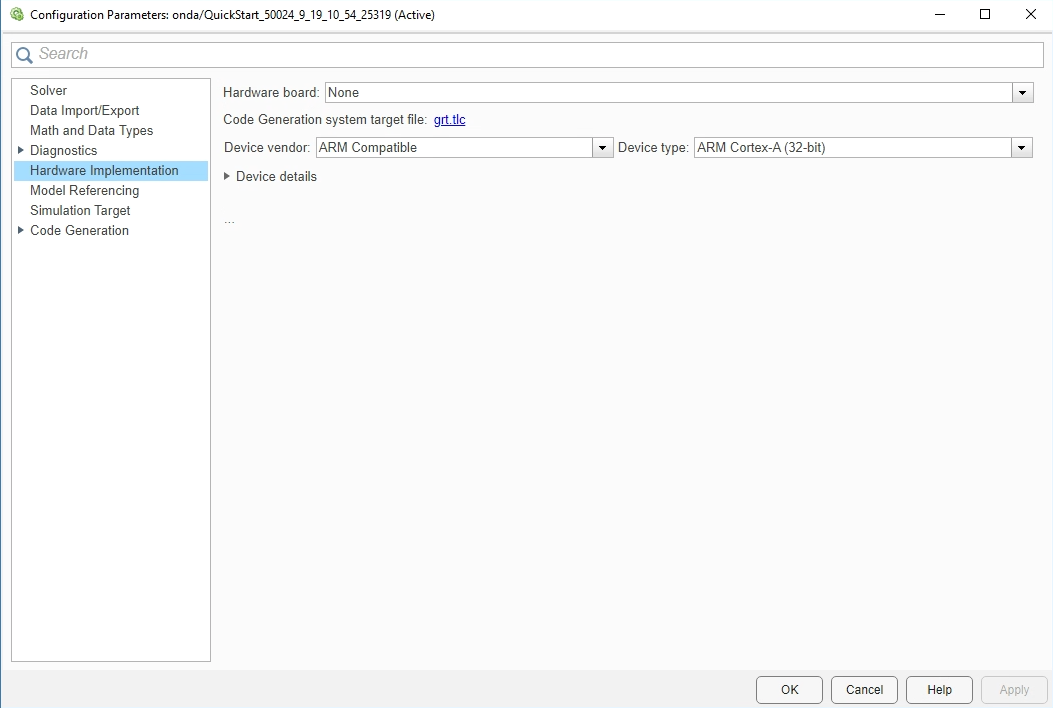
\includegraphics[width=0.8\textwidth]{fig/especifico_2/paso_a_paso_mtmt/configuration_parameters_processor.png}
    \caption{Selección del procesador y la familia del procesador}
    \label{fig:pestana_config_procesador}
\end{figure}

Continuando en la sección de configuración de parámetros ahora debemos de ir a la pestaña llamada implementación de hardware o bien Hardware Implementation, en donde deberemos de colocar los datos de Device Vendor el cual hace referencia al tipo de procesador que contiene la tarjeta de desarrollo, para nuestro caso sería ARM Compatible y el Device Type que seria a la familia que pertenece el procesador, para nuestro caso sería un ARM Cortex-A de 32-bits tal y como se muestra en la Figura \ref{fig:pestana_config_procesador}.


\subsubsection{Selección del tipo de archivo de construcción}

Anteriormente configuramos los parámetros de tiempo de operación y procesador de la tarjeta de desarrollo, ahora debemos de configurar el tipo de archivo que se utilizara para la generación de los archivos binarios, como se deberá de realizar una compilación cruzada se debe de elegir un tipo de archivo el cual nos permita compilar los binarios para la ejecución del sistema sin importar el sistema operativo de la máquina host. Es por esto que se debe de seleccionar en la pestaña de Code Generation el Toolchain denominado CMake tal y como se muestra en la Figura \ref{fig:pestana_config_output_file}, además de esto se debe de marcar tanto la opción denominada como Generate code only, como Package code and artifacts, esta última nos genera como salida un archivo comprimido con todos los requerimientos de la aplicación para poder ser construida.


\begin{figure}[h!]
    \centering
    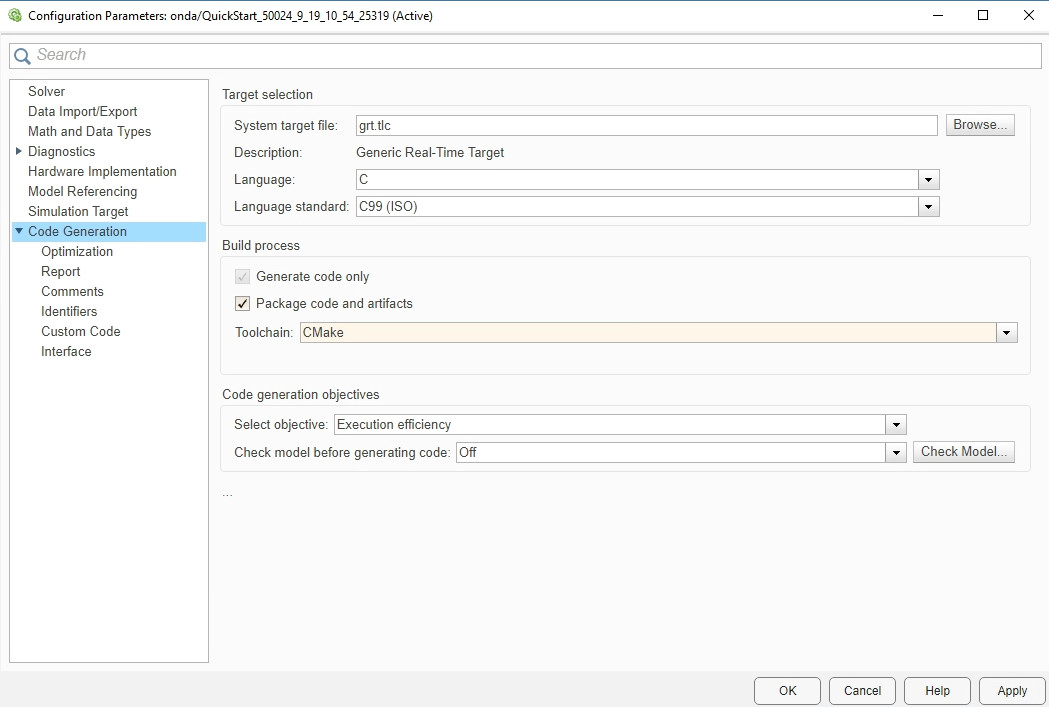
\includegraphics[width=0.8\textwidth]{fig/especifico_2/paso_a_paso_mtmt/configuration_output_file.png}
    \caption{Selección del tipo de archivo de construcción}
    \label{fig:pestana_config_output_file}
\end{figure}

\subsubsection{Generación de archivos de compilación}

Una vez configurados todos los parámetros mencionados anteriormente debemos de proceder con la construcción de los archivos, para esto se debe de ir a la barra de tareas a la opción denominada como generar código, la misma se puede observar en la Figura \ref{fig:pestana_c_code} bajo el nombre de Build.

\subsection{Contenedor para compilación de los binarios}

Para poder generar la compilación cruzada es necesario crear un contenedor para poder utilizar Ubuntu 20.04, ya que esta versión es la que presenta mayor compatibilidad con las dependencias contenidas en el flujo de trabajo de Yocto Project que se utiliza. 


\begin{lstlisting}[language=bash, caption={Instalacion de docker, Linux}, label=lst:install_docker]
    sudo apt install docker.io
\end{lstlisting}

\begin{lstlisting}[language=bash, caption={Instalacion de Ubuntu 20.04, Linux}, label=lst:install_20_04_ubuntu]
    sudo docker run -it ubuntu:20.04 /bin/bash
\end{lstlisting}

Para poder generar este contenedor primeramente se debe de satisfacer la dependencia de tener instalado docker.io, esto se logra por medio del comando que se muestra en \ref{lst:install_docker},seguido de esto, se puede hacer uso del comando \ref{lst:install_20_04_ubuntu} el cual se encarga de construir la máquina dentro del entorno del contenedor. Este último comando se encarga de descargar la imagen de Ubuntu 20.04, crea y ejecuta un contenedor en modo interactivo además de proporcionar acceso al terminal del contenedor, donde puedes ejecutar comandos como si fuera una máquina virtual con Ubuntu 20.04.

\subsubsection{Instalación de programas en el contenedor}

\begin{lstlisting}[language=bash, caption={Instalacion del compilador cruzado, Linux}, label=lst:cross_compiler]
    sudo apt install gcc-arm-linux-gnueabihf
\end{lstlisting}

\begin{lstlisting}[language=bash, caption={Instalacion de CMake, Linux}, label=lst:cmake]
    sudo apt install cmake
\end{lstlisting}

\begin{lstlisting}[language=bash, caption={Instalacion de build essential, Linux}, label=lst:build_essential]
    sudo apt install build-essential
\end{lstlisting}

Una vez generado el contenedor debemos de instalar en el mismo el compilador cruzado que para nuestros efectos será arm-linux-gnueabihf-gcc, esto lo podemos hacer mediante el comando que se muestra en \ref{lst:cross_compiler},  CMake el cual es una herramienta de construcción multiplataforma y de código abierto que se utiliza para gestionar la construcción de software utilizando un enfoque basado en proyectos y finalmente build-essential las cuales son herramientas que nos ayudaran a compilar el programa generado en \ref{subsec:simulink_coder} para la arquitectura del procesador.

\begin{figure}[h!]
    \centering
    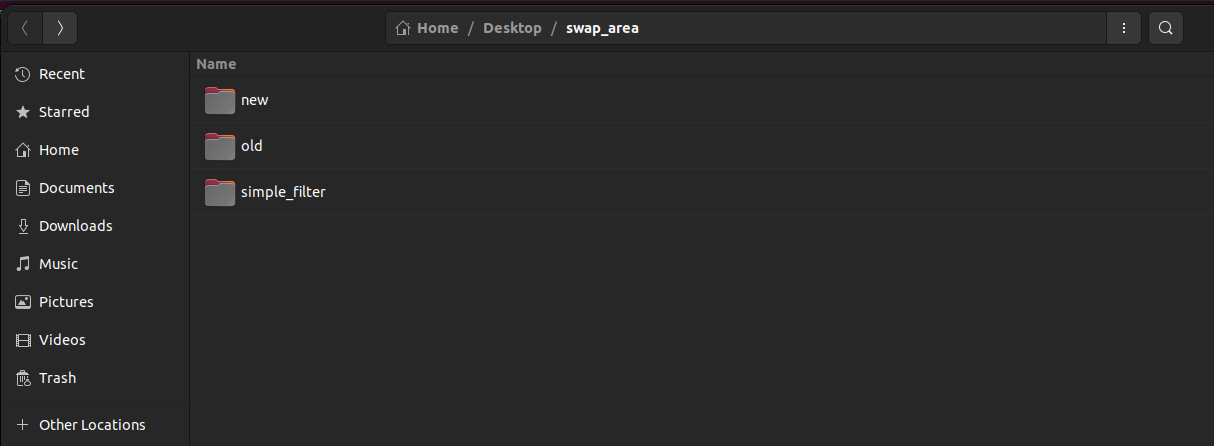
\includegraphics[width=0.8\textwidth]{fig/especifico_2/paso_a_paso_mtmt/root_folder.png}
    \caption{Archivo comprimido en el directorio swap\_area}
    \label{fig:pestana_swap_area}
\end{figure}

\begin{lstlisting}[language=bash, caption={Copiar archivos al contenedor, Linux}, label=lst:copy_to_container]
    sudo docker cp /direccion/del/archivo 
    <id_de_contenedor>:/direccion/del/contenedor
\end{lstlisting}

\begin{lstlisting}[language=bash, caption={Copiar archivos del contenedor, Linux}, label=lst:copy_from_container]
    sudo docker cp <id_de_contenedor>:/direccion/del/contenedor
    /direccion/del/archivo
\end{lstlisting}

Seguido de esto se debe de copiar el archivo comprimido generado en \ref{subsec:simulink_coder}, al contenedor con Ubuntu. Primeramente colocaremos el archivo comprimido en un directorio llamado swap\_area, tal y como se muestra en \ref{fig:pestana_swap_area}. Seguido de esto se debe de descomprimir el archivo. Una vez descomprimido el archivo, como se mencionó anteriormente, lo enviaremos al contenedor haciendo uso del comando \ref{lst:copy_to_container}.

\subsection{Compilación de los binarios}\label{subsec:compilacion_binario}

\begin{lstlisting}[language=bash, caption={Compilacion del programa, Linux}, label=lst:build_cmake_file]
    cmake -DCMAKE_C_COMPILER=arm-linux-gnueabihf-gcc 
    CMakeLists.txt -DMATLAB_ROOT=/home/test/simple_filter/R2024b/
\end{lstlisting}

\begin{figure}[h!]
    \centering
    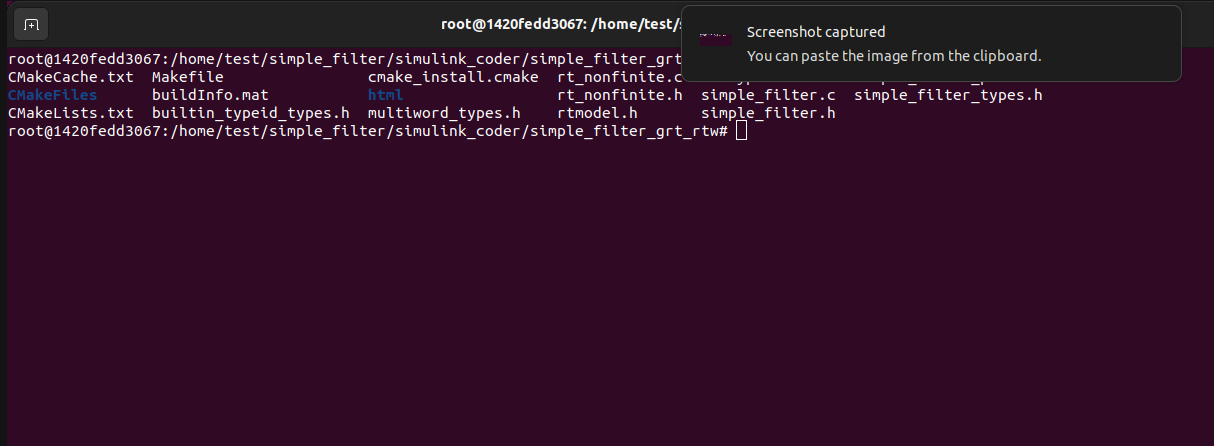
\includegraphics[width=0.8\textwidth]{fig/especifico_2/paso_a_paso_mtmt/cmake_file.png}
    \caption{Make File}
    \label{fig:make_file}
\end{figure}


\begin{figure}[h!]
    \centering
    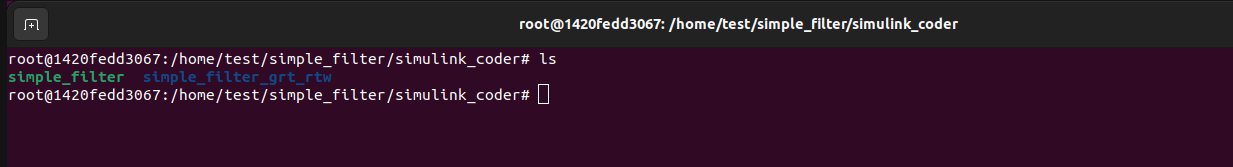
\includegraphics[width=0.8\textwidth]{fig/especifico_2/paso_a_paso_mtmt/binario_compilado.png}
    \caption{Binario llamado simple\_filter}
    \label{fig:binario_compilado}
\end{figure}

Para la compilación del archivo binario se deberá hace uso del comando \ref{lst:build_cmake_file} por el cual se construirá el Makefile, tal y como se muestra en la Figura \ref{fig:make_file}, una vez generado el Makefile se ejecutó el comando make el cual da como salida los binarios requeridos para la ejecución del programa. Los mismos se observan como se muestra en la Figura \ref{fig:binario_compilado}.

Una vez compilado el archivo binario, se puede continuar con el flujo que se presenta en el diagrama que se muestra en la Figura \ref{fig:diagrama_flujo_trabajo}, lo cual sería la implementación de los binarios en una imagen de yocto.


\section{Flujo de Trabajo Herramienta desarrollada por mi persona}

Como se pudo observar anteriormente se realizó la compilación cruzada de un caso de estudio, el mismo ahora se debe de implementar en un sistema operativo a la medida mediante el flujo de trabajo de Yocto Project, como se mencionó en \ref{subsec:yocto}, Yocto Project es un marco de trabajo utilizado para el desarrollo de sistemas embebidos especializado en la construcción de distribuciones de Linux a la medida. 

\begin{figure}[h!]
    \centering
    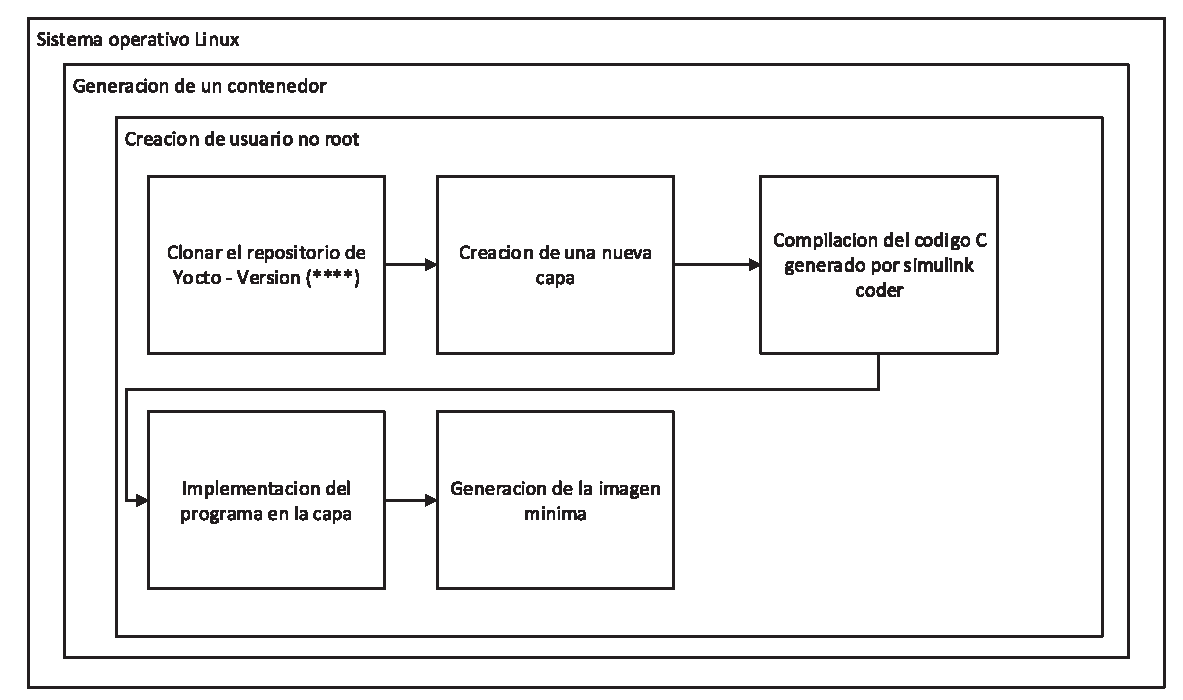
\includegraphics[width=0.8\textwidth]{fig/especifico_2/Flujo de trabajo de mi idea.pdf}
    \caption{Flujo de trabajo Yocto}
    \label{fig:flujo_yocto}
\end{figure}

En el desarrollo de esta seccion se muestran los pasos que se siguieron para la generación de una imagen mínima, la integración de una capa personalizada con el binario generado en \ref{subsec:compilacion_binario} y la implementación de la misma en la tarjeta de desarrollo seleccionada.

\subsection{Sistema operativo para desarrollo}

Como sistema operativo de desarrollo se utilizó Ubuntu 22.04 LTS, en una computadora con las siguientes características:

\begin{itemize}
    \item Procesador - Intel Corei9-13980HX 
    \item Almecenamiento - 500 GB
    \item Memoria RAM - 16 GB 
\end{itemize}

\subsection{Generación de un contenedor}

Para el desarrollo del marco de trabajo de Yocto se decidió implementar un contenedor, esto debido a que la versión de Yocto para la cual se encontraba un paquete de soporte para la tarjeta de desarrollo es Yocto Zeus 3.0, este fue liberado en octubre del 2019, por tanto no era soportado por la versión de Linux del computador de desarrollo, es por esto que se tomó la decisión de utilizar un contenedor el cual ejecutara la versión de Ubuntu 16.04 LTS. 

\begin{lstlisting}[language=bash, caption={Instalacion de Ubuntu 16.04}, label=lst:install_16_04_ubuntu]
    sudo docker run -it ubuntu:16.04 /bin/bash
\end{lstlisting}

Para la generación del contenedor se hace uso del comando que se muestra en \ref{lst:install_16_04_ubuntu}, el cual se encarga de darnos un contenedor con Ubuntu 16.04 LTS.Ademas de esto debemos de instalar algunos requerimientos como lo son:

\begin{itemize}
    \item tree : para poder visualizar árboles de dependencia
    \item vim : para poder editar archivos de texto
    \item etc \dots
\end{itemize}

\subsubsection{Creación de un usuario no root}

Para el uso del marco de trabajo de Yocto se debe de generar un usuario no root, esto principalmente por razones de seguridad y manejo adecuado de permisos. El usuario se puede generar por medio de los siguientes comandos:

\begin{lstlisting}[language=bash, caption={Generacion de usuario no root, Linux}, label=lst:no_root_user]
    apt - get install -y sudo
    useradd - ms/bin/bash myuser
    echo "myuser:password" | chpasswd
    usermod - aG sudo myuser
\end{lstlisting}

De forma que según el comando observado en \ref{lst:no_root_user}, en la primera línea instalamos sudo, seguido de esto en la segunda línea se agrega el usuario denominado "myuser", en la tercera línea se genera una contraseña para este usuario la cual se define como "chpasswd", finalmente se agrega en el archivo usermod el nuevo usuario. 

\begin{lstlisting}[language=bash, caption={Iniciar usuario no root, Linux}, label=lst:no_root_user_log]
    su - myuser
\end{lstlisting}


Cada vez que iniciemos el contenedor siempre lo haremos como usuario root, para poder iniciar con el usuario no root llamado "myuser" se debe de hacer uso del comando que se muestra en \ref{lst:no_root_user_log}.

\subsection{Yocto Project}

Como se observó en \ref{subsec:yocto}, yocto presenta flexibilidades a la hora de configurar un sistema permitiendo al desarrollador seleccionar paquetes específicos y personalizar el sistema operativo.

\begin{lstlisting}[language=bash, caption={Requerimientos Yocto Zeus, Linux}, label=lst:yocto_requirements]
    sudo apt - get install gawk wget git - core diffstat unzip texinfo
    gcc - multilib build - essential chrpath socat cpio python python3
    python3 - pip python3 - pexpect xz - utils debianutils 
    iputils - ping python3 - git python3 - jinja2 
    libegl1 - mesa libsdl1 .2 - dev pylint3 xterm
\end{lstlisting}

Para que el mismo funcione de forma correcta debemos de instalar los requerimientos del marco de trabajo los cuales se pueden observar en \ref{lst:yocto_requirements}.

\begin{lstlisting}[language=bash, caption={Version de Yocto}, label=lst:yocto_clone]
    git clone -b zeus https://git.yoctoproject.org/git/poky
    cd poky
\end{lstlisting}

\begin{lstlisting}[language=bash, caption={BSP para Zedboard}, label=lst:yocto_zedboard]
    git clone -b zeus https://github.com/Xilinx/meta-xilinx
    git clone -b zeus https://github.com/openembedded/meta-openembedded.git
\end{lstlisting}

La versión de yocto a utilizar se debe de clonar de \ref{lst:yocto_clone}, seguido de esto se debe de ir a la rama de la versión Yocto Zeus. Además de clonar este repositorio se debe de ingresar al directorio denominado poky y clonar dentro del repositorio \ref{lst:yocto_zedboard} el cual contiene en su rama llamada Zeus la versión de paquete de soporte para la tarjeta requerida para generar una imagen para la tarjeta de desarrollo seleccionada.

\begin{lstlisting}[language=bash, caption={Configuraciones adicionales, Yocto}, label=lst:aditional_config]
    source oe - init - build - env
    
    echo "MACHINE ??=\"zedboard-zynq7\"" >> conf/local.conf
    echo "IMAGE_FEATURES +=\"package-management\"" >> conf/local.conf
    echo "DISTRO_HOSTNAME =\"zynq\"" >> conf/local.conf
    
    bitbake-layers add-layer ../meta-xilinx/meta-xilinx-bsp/
    bitbake-layers add-layer ../meta-openembedded/meta-oe/
\end{lstlisting}

Algunas configuraciones adicionales que se deben de realizar se muestran en \ref{lst:aditional_config}.

\subsection{Creación de una capa de yocto}

\begin{lstlisting}[language=bash, caption={"Print Working Directory",Linux}, label=lst:pwd]
    pwd
\end{lstlisting}

\begin{lstlisting}[language=bash, caption={Inicializar ambiente, Yocto}, label=lst:yocto_ambient_set]
    source oe-init-build-env
\end{lstlisting}

Para la generación de una capa de yocto primero debemos de estar seguros que nos encontramos en el directorio denominado POKY, esto lo podemos verificar por medio del uso del comando \ref{lst:pwd}, seguido de esto se debe de inicializar el entorno de desarrollo esto mediante el comando que se muestra en \ref{lst:yocto_ambient_set}, este se encarga de generar todos los archivos necesarios para poder hacer uso de las variables de entorno con las cuales opera el marco de trabajo de Yocto.

\begin{lstlisting}[language=bash, caption={Generar nueva capa, Yocto }, label=lst:yocto_new_layer]
    bitbake-layers create-layer <nombre-de-la-capa>
\end{lstlisting}

\begin{figure}[h!]
    \centering
    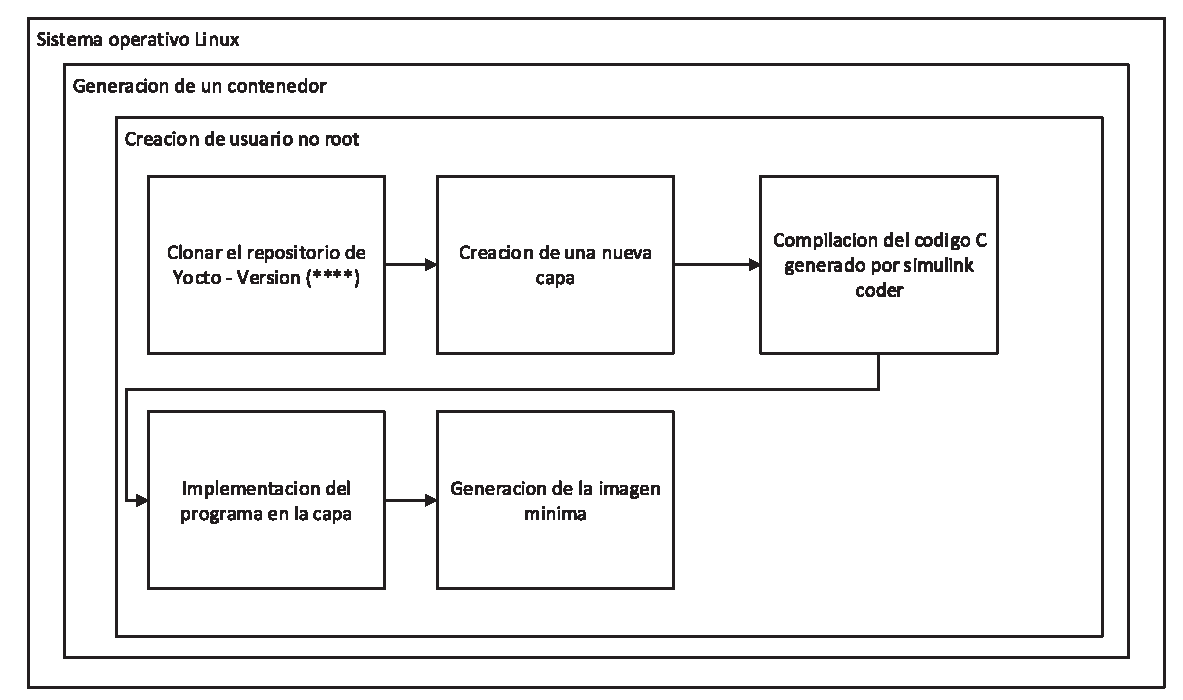
\includegraphics[width=0.8\textwidth]{fig/especifico_2/Flujo de trabajo de mi idea.pdf}
    \caption{Árbol de directorios de la capa}
    \label{fig:arbol_capa_custom_yocto}
\end{figure}

\begin{lstlisting}[language=bash, caption={Agregar nueva capa, Yocto }, label=lst:add_new_layer]
    bitbake-layers add-layer ../<nombre-de-la-capa>
\end{lstlisting}

Seguido de esto se debe de utilizar el comando que se muestra en \ref{lst:yocto_new_layer} el cual se encargara de generar el árbol de directorios que se puede observar en la Figura \ref{fig:arbol_capa_custom_yocto}. Una vez implementado este comando se debe de hacer uso del comando que se muestra en \ref{lst:add_new_layer} para poder agregar la capa al archivo denominado bblayers.conf el cual contiene todas las rutas de acceso a las capas requeridas para generar la imagen.

\subsection{Caso de estudio}

En esta sección se integrará el caso de estudio generado en \ref{subsec:compilacion_binario}, a un sistema operativo a la medida por medio del marco de trabajo de Yocto Project, primeramente se generara una capa personalizada, seguido de esto se generara el archivo de instalación con el cual la capa personalizada pasara a ser parte del sistema de archivos del sistema embebido, también se generara la imagen mínima la cual consiste en un sistema de arranque y el sistema de archivos y finalmente se implementaran estos en la tarjeta de desarrollo seleccionada en \ref{ch:especifico1}.

\subsection{Integración del programa generado a la capa de Yocto}

Para la implementación del binario generado en \ref{subsec:compilacion_binario}, se deben de generar algunos directorios, esto con el objetivo de mantener un entorno limpio y ordenado. Para contener todos los directorios que se deben de crear, se genera un directorio llamado "recipes-core" el cual dentro del mismo deberá de contener un directorio llamado "sistema\_control" el cual se encargara de contener el archivo de configuración de la capa llamado "sistema\_control.bb"; este archivo se genera mediante el comando que se observa en \ref{lst:yocto_new_layer}, además de generar este archivo se debe de crear un directorio llamado "files" que será el encargado de contener el archivo binario compilado en \ref{subsec:compilacion_binario}.

\subsubsection{sistema\_control.bb}

Como se mencionó anteriormente el archivo llamado sistema\_control.bb es el encargado de la configuración de la capa, el mismo contiene los comandos de instalación y la dirección en donde se encontraran los binarios en el sistema de archivos de la imagen del sistema embebido.

\begin{figure}[h!]
    \centering
    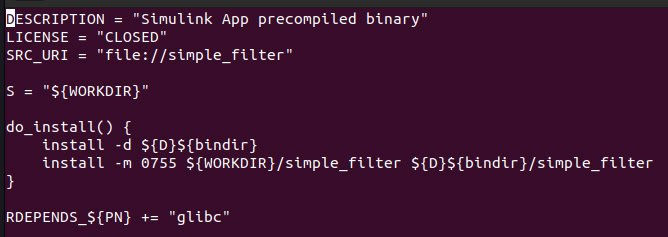
\includegraphics[width=0.8\textwidth]{fig/especifico_2/bbfilestructure.jpg}
    \caption{Estructura del archivo sistema\_control.bb}
    \label{fig:estructura_archivo_bb}
\end{figure}

La estructura que debe de contener ese archivo para instalar binarios en el sistema son las que se pueden observar en la Figura \ref{fig:estructura_archivo_bb}.

\subsection{Generación de la imagen mínima}\label{subsec:generacion_imagen_minima}

\begin{lstlisting}[language=bash, caption={Generar archivos de desarrollador, Yocto }, label=lst:yocto_developer_image]
    bitbake-layers add-layer ../<nombre-de-la-capa>
\end{lstlisting}

Antes de generar la imagen mínima se debe de tener en consideración ejecutar la línea de comando que se muestra en \ref{lst:yocto_developer_image}, esto con el fin de generar archivos de desarrollo en lugar de archivos de imagen en formato iso. Una vez generados estos cambios se debe de iniciar de nuevo el entorno por medio del comando \ref{lst:yocto_ambient_set}, seguido de esto se deberá de ejecutar el comando de "bitbake core-image-minimal" el cual se encarga de comenzar a generar la imagen mínima.

\subsection{Implementación de la imagen mínima en la tarjeta de desarrollo Zedboard}

Para la implementación de la imagen mínima desarrollada en \ref{subsec:generacion_imagen_minima} en la tarjeta de desarrollo, se deben de desarrollar los siguientes pasos en la máquina Host:

\begin{enumerate}
    \item Se debe de formatear la tarjeta SD de al menos 4 GB, las particiones de la misma se tienen que observar de la siguiente forma 
    \begin{itemize}
        \item raíz = 100 MB FAT 32
        \item sistema de archivos = 3.5 GB ext6(linux filesystem format)
        \end{itemize} 
\end{enumerate}

Seguido de esto se debe de ir a la ruta (ruta donde se encuentran los archivos de imagen de la zedboard), mientras que en la máquina host se debe de ir a la ruta seleccionada para almacenar los archivos temporalmente y se deben de copiar los archivos del contenedor a la máquina host mediante el comando que se muestra en \ref{lst:copy_from_container}, esto con el objetivo de poder enviar los archivos a la tarjeta SD más adelante.

\begin{lstlisting}[language=bash, caption={Copiar archivos root, Linux}, label=lst:copy_root]
    sudo cp boot.bin boot.scr 
    core-image-minimal-zedboard-zynq7.cpio.gz.u-boot
     u-boot.img uEnv.txt uImage zynq-zed.dtb /media/root
\end{lstlisting}

\begin{lstlisting}[language=bash, caption={Copiar sistema de archivos, Linux}, label=lst:copy_fs]
    sudo cp core-image-minimal-zedboard-zynq7.tar.gz /mnt/partition2
\end{lstlisting}

Para el sistema Root se deberán de copiar los archivos mediante el comando que se muestra en \ref{lst:copy_root}, por otro lado en la partición denominada FileSystem se debe de copiar el archvivo "core-image-minimal-zedboard-zynq7.tar.gz" mediante el uso del comando que se muestra en \ref{lst:copy_fs}.

\subsection{Conexión de la tarjeta de desarrollo con el computador host}

Como protocolo de comunicación se establece de primera mano UART, el cual como se mencionó en \ref{sec:protocolos_de_comunicacion} consiste en un protocolo de comunicación serie que permite la transmisión y recepción de datos de manera asíncrona entre dos dispositivos y en el caso de la tarjeta de desarrollo se conecta según se muestra en el diagrama de la Figura \ref{fig:puertos_zedboard}, mediante el uso del puerto marcado como "S" en el diagrama. Para poder leer la consola se hace uso de Minicom el cual se encarga de la emulación de terminal en Linux que permite la comunicación serie con dispositivos a través de puertos seriales.

\begin{figure}[h!]
    \centering
    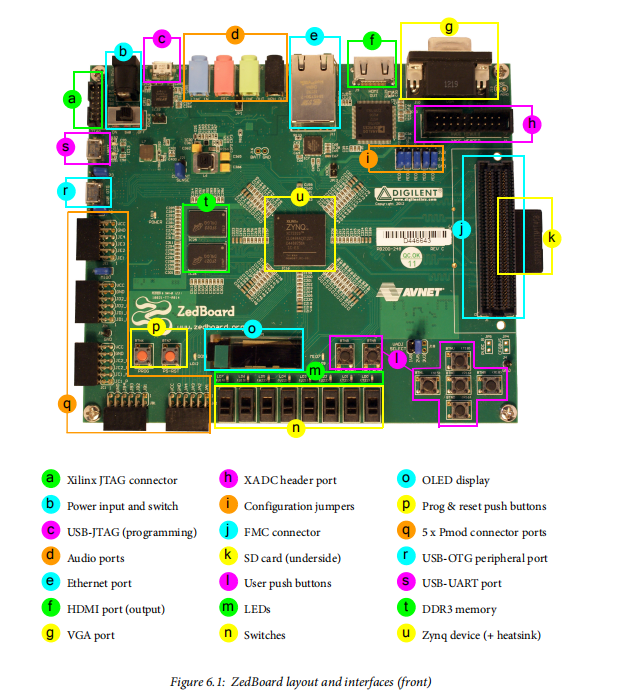
\includegraphics[width=0.8\textwidth]{fig/especifico_2/154140ZedBoard.png}
    \caption{Puertos tarjeta de desarrollo Zedboard}
    \label{fig:puertos_zedboard}
\end{figure}


Una vez que se estableció la conexión por medio de SSH el cual como se menciona en \ref{sec:protocolos_de_comunicacion}, consiste en protocolo de comunicación en red que permite el acceso remoto seguro a sistemas, proporcionando autenticación y encriptación de datos, ya que es mejor que UART para comunicaciones remotas porque proporciona autenticación y encriptación, garantizando la seguridad de los datos transmitidos, mientras que UART es un protocolo simple y sin mecanismos de seguridad, adecuado solo para comunicaciones locales y de corto alcance. 

El diagrama de este protocolo de comunicación se puede observar en \ref{fig:puertos_zedboard}, el cual se logra mediante la conexión al puerto denominado en el diagrama como .


\subsection{Ejecución del caso de estudio y resultados}

Una vez implementada la imagen de Yocto en la tarjeta de desarrollo se puede ejecutar el caso de estudio. Para esto será necesario dirigirnos al directorio en el cual se instaló el archivo binario, el mismo se encuentra en la ruta xxxxx. Una vez encontrado el archivo basta con ejecutarlo mediante el uso del nombre del mismo "simple\_filter". Cuando el archivo se ejecuta genera dos archivos de salida llamados xxx y xxx, mediante el uso del programa en Python desarrollado se pueden leer los archivos generados y crear gráficos a partir de los mismos. Los resultados se deben de transmitir al computador por medio del comando \ref{lst:copy_ssh}.

\begin{lstlisting}[language=bash, caption={Copiar archivo por protocolo SSH, Linux}, label=lst:copy_ssh]
    scp user@ip:/ruta/del/archivo/zedboard .
\end{lstlisting}

\begin{figure}[htbp]
    \centering
    \begin{subfigure}[b]{0.45\textwidth}
        \centering
        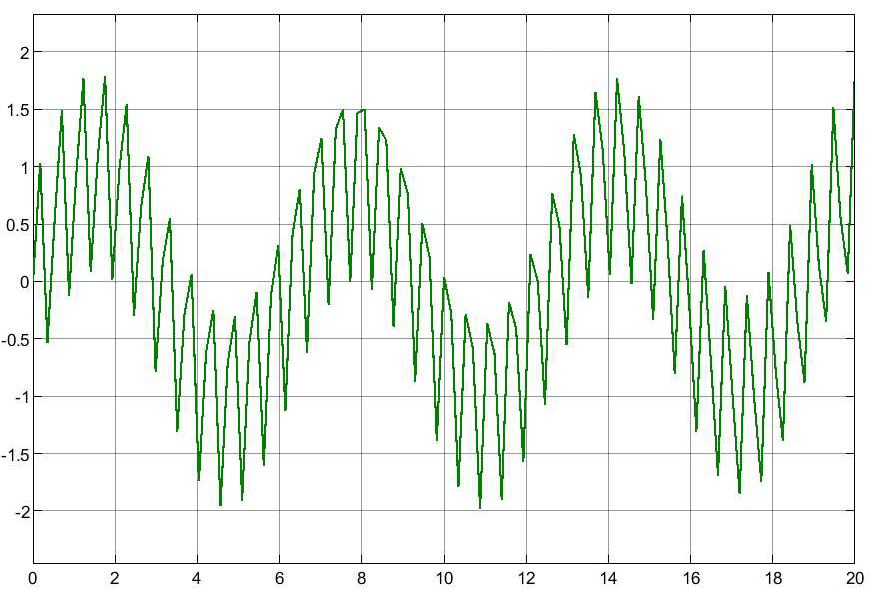
\includegraphics[width=\textwidth]{fig/especifico_2/onda_modulada.pdf}
        \caption{Ondas Moduladas}
        \label{fig:onda_modulada_zedboard}
    \end{subfigure}
    \hfill
    \begin{subfigure}[b]{0.45\textwidth}
        \centering
        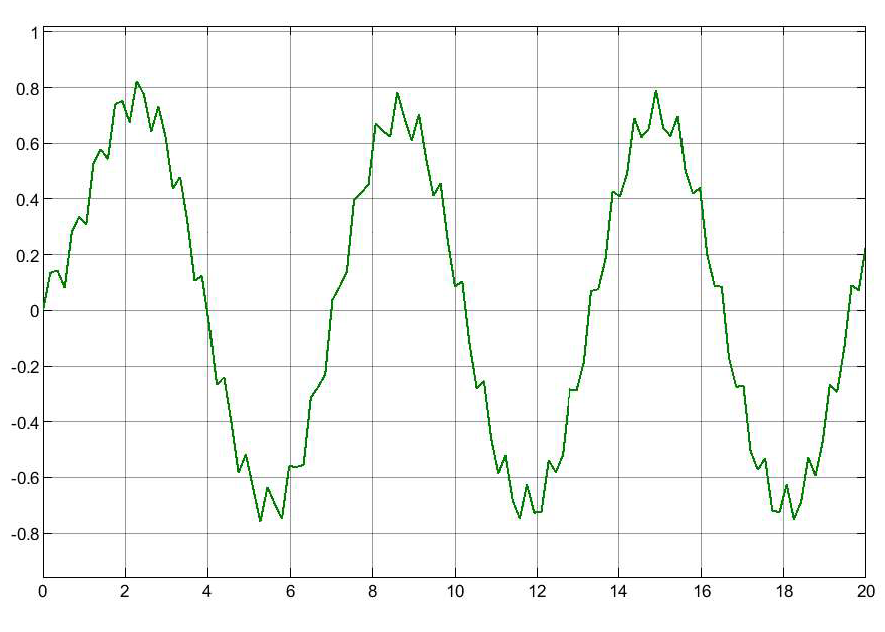
\includegraphics[width=\textwidth]{fig/especifico_2/onda_filtrada.pdf}
        \caption{Onda resultante luego de la función de transferencia}
        \label{fig:onda_filtrada_zedboard}
    \end{subfigure}
    \caption{Salida resultante del diagrama mostrado en la Figura \ref{fig:diagrama_matlab_simulink_graficos}}
    \label{fig:salida_resultante_diagrama_graficos_zedboard}
\end{figure}

\subsection{Comparación de resultados}

Como se pudo observar, con la comparación realizada, obtenemos que los datos tiene una desviación de xxxxx además de xxxxxx, es por esto que podemos determinar que la implementación de sistemas de control es viable según lo demuestra el caso de estudio.



\section{Reflexión final}
  \chapter{Caso de estudio IMU y PID}
\label{ch:especifico3}

\section{Caso de estudio 2 - IMU}

Como caso de estudio de implementación de una Unidad de medición inercial, IMU por sus siglas en Ingles, se siguió el uso del modelo que se presenta en \cite{mathworks2024imu}. Este ejemplo muestra cómo generar y fusionar datos de sensores IMU usando MATLAB Simulink. Permitiendo modelar con precisión el comportamiento de un acelerómetro, un giroscopio y un magnetómetro, además de poder fusionar sus salidas para calcular la orientación.

Una IMU es un grupo de sensores que incluye un acelerómetro para medir aceleración y un giroscopio para medir velocidad angular. Frecuentemente, también se incluye un magnetómetro para medir el campo magnético de la Tierra. Cada uno de estos tres sensores produce una medición de tres ejes, constituyendo una medición de 9 ejes en total. Ademas de esto un Sistema de Referencia de Actitud y Rumbo (AHRS, por sus siglas en inglés) toma las lecturas de sensores de 9 ejes y calcula la orientación del dispositivo. Esta orientación se da en relación con el marco NED, donde N es la dirección del Norte Magnético. El bloque AHRS en Simulink logra esto usando una estructura de filtro de Kalman indirecto \cite{mathworks2024imu}.

\subsection{Implementación en MATLAB Simulink}

\begin{figure}[h!]
    \centering
    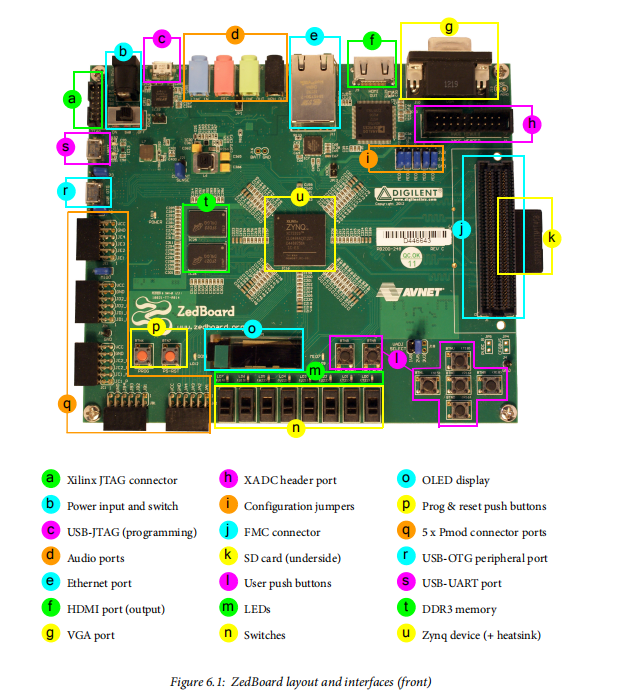
\includegraphics[width=0.8\textwidth]{fig/especifico_2/154140ZedBoard.png}
    \caption{Diagrama completo del caso de estudio 2 - IMU \cite{mathworks2024imu}}
    \label{fig:caso_de_estudio_2_IMU}
\end{figure}


Como se puede observar en la Figura \ref{fig:caso_de_estudio_2_IMU}, este es el caso de estudio que se propone en \cite{mathworks2024imu}, a este caso de estudio se le deben de realizar unas modificaciones de acuerdo al funcionamiento deseado que se tiene para este caso de estudio, siempre generando datos en el ámbito de simulación en MATLAB para luego contrastar los mismos con los datos obtenidos en la ejecución del modelo en la tarjeta de desarrollo seleccionada.

\subsection{Bloques utilizados para la implementación}

Los bloques utilizados se obtienen en la librería de bloques de MATLAB Simulink. A continuación se muestran los bloques requeridos, asi como la configuración de los mismos para la correcta operación del modelo. La implementación del sistema se divide en dos partes, el primer parte se encarga de generar los archivos necesarios para la operación del sistema mientras que la segunda parte del sistema se encarga de leer los archivos con los datos y generar los dos archivos de salida del programa.

\subsubsection{Sistema para la generación de archivos}

Este sistema es el encargado de generar los archivos de entrada, estos mismos contienen los datos de tiempo y valores para la correcta implementación del sistema

\begin{figure}[h!]
    \centering
    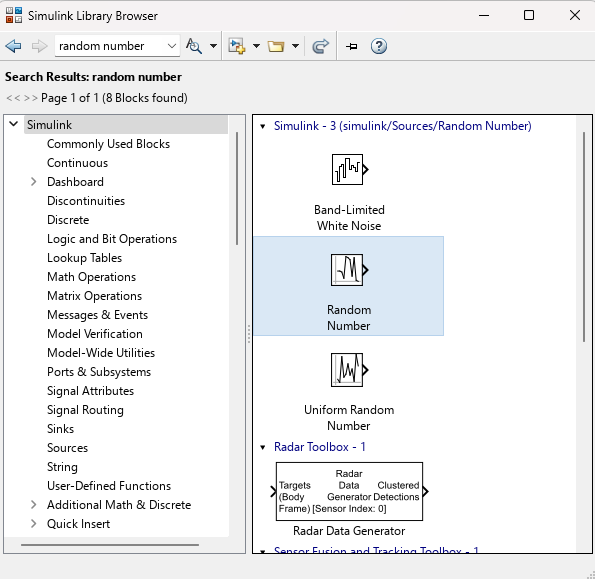
\includegraphics[width=0.45\textwidth]{fig/Capitulo5/Caso_de_estudio_IMU/Generador_de_archivos/libreria_de_bloques_aceleracion_lineal.png}
    \caption{Librería de bloques - Aceleración Lineal}
    \label{fig:lib_bloques_linear_acceleration}
\end{figure}

\begin{figure}[h!]
    \centering
    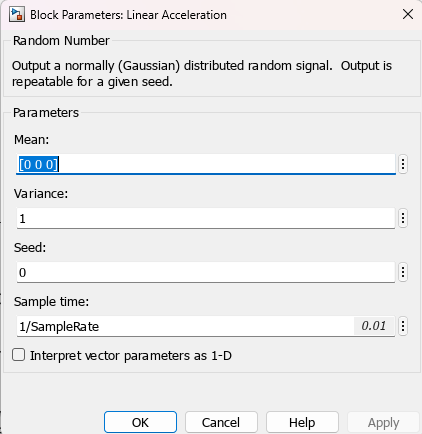
\includegraphics[width=0.45\textwidth]{fig/Capitulo5/Caso_de_estudio_IMU/Generador_de_archivos/configuracion_bloque_aceleracion_lineal.png}
    \caption{Configuración del bloque aceleración lineal}
    \label{fig:lib_bloques_config_linear_acceleration}
\end{figure}

\begin{figure}[h!]
    \centering
    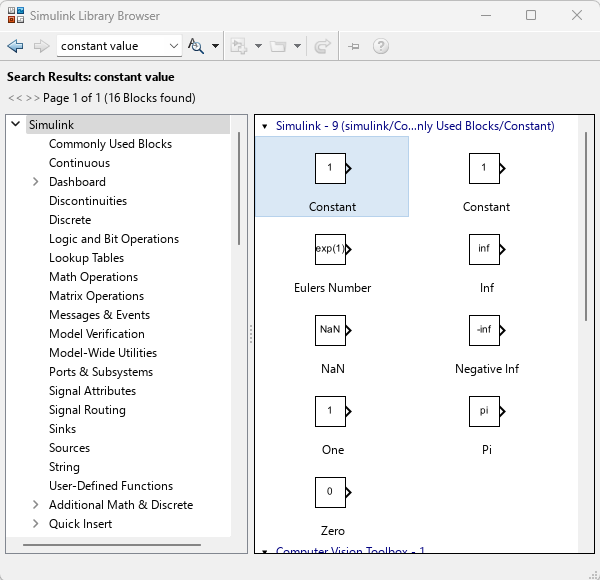
\includegraphics[width=0.45\textwidth]{fig/Capitulo5/Caso_de_estudio_IMU/Generador_de_archivos/libreria_de_bloques_constante_velocidad_angular.png}
    \caption{Librería de bloques - Velocidad Angular}
    \label{fig:lib_bloques_angular_velocity}
\end{figure}

\begin{figure}[h!]
    \centering
    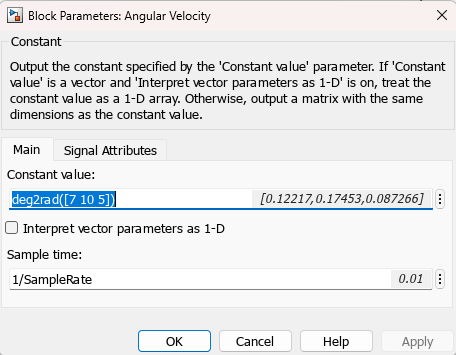
\includegraphics[width=0.45\textwidth]{fig/Capitulo5/Caso_de_estudio_IMU/Generador_de_archivos/configuracion_bloque_velocidad_angular.png}
    \caption{Configuración del bloque velocidad angular}
    \label{fig:lib_bloques_config_angular_velocity}
\end{figure}

\begin{figure}[h!]
    \centering
    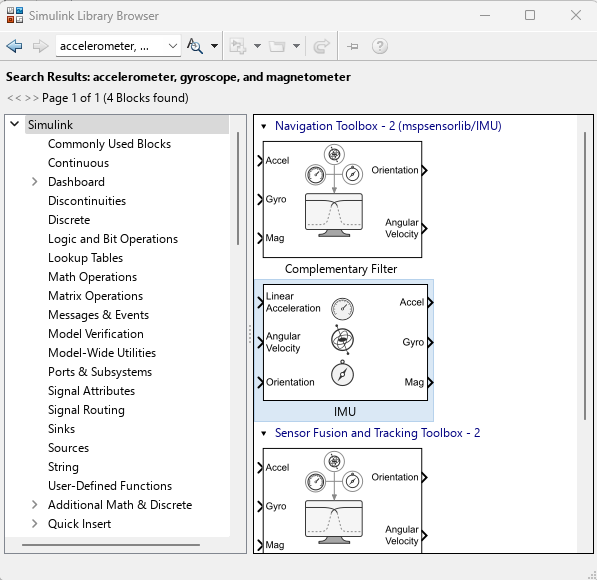
\includegraphics[width=0.45\textwidth]{fig/Capitulo5/Caso_de_estudio_IMU/Generador_de_archivos/libreria_de_bloques_IMU.png}
    \caption{Librería de bloques - IMU}
    \label{fig:lib_bloques_IMU}
\end{figure}


\begin{figure}[h!]
    \centering
    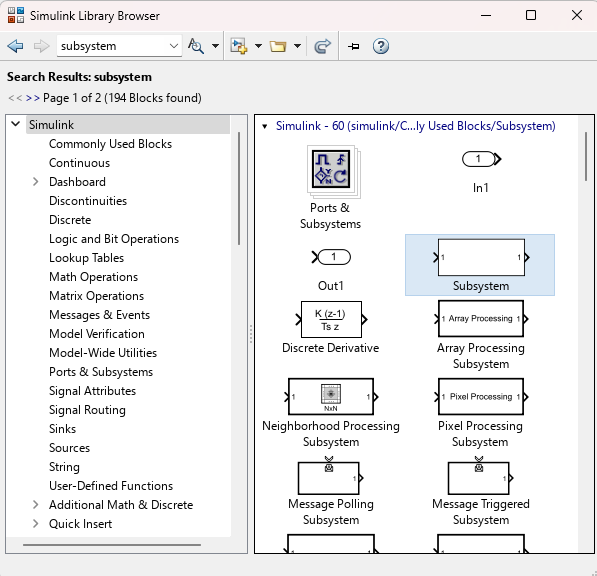
\includegraphics[width=0.45\textwidth]{fig/Capitulo5/Caso_de_estudio_IMU/Generador_de_archivos/libreria_de_bloques_subsistema_integracion_velocidad_angular.png}
    \caption{Librería de bloques - Integrador}
    \label{fig:lib_bloques_integrador}
\end{figure}

\begin{figure}[h!]
    \centering
    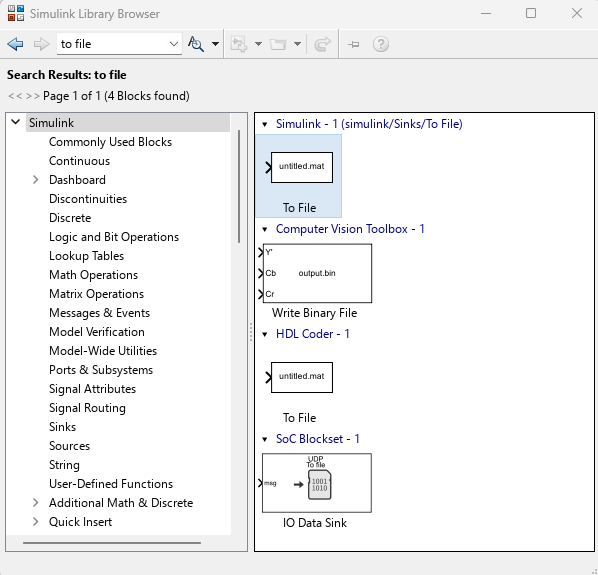
\includegraphics[width=0.45\textwidth]{fig/Capitulo5/Caso_de_estudio_IMU/Generador_de_archivos/libreria_de_bloques_to_file.png}
    \caption{Librería de bloques - Guardar en archivo}
    \label{fig:lib_bloques_to_file_IMU}
\end{figure}

\subsubsection{Sistema para la lectura e interpretación de los archivos generados previamente}

\begin{figure}[h!]
    \centering
    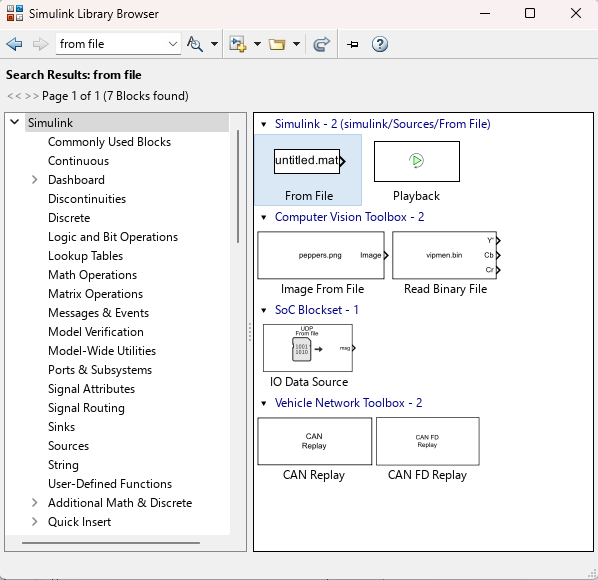
\includegraphics[width=0.45\textwidth]{fig/Capitulo5/Caso_de_estudio_IMU/Generador_de_salidas/libreia_de_bloques_from_file.png}
    \caption{Librería de bloques - Leer de archivo}
    \label{fig:lib_bloques_from_file_IMU}
\end{figure}

\begin{figure}[h!]
    \centering
    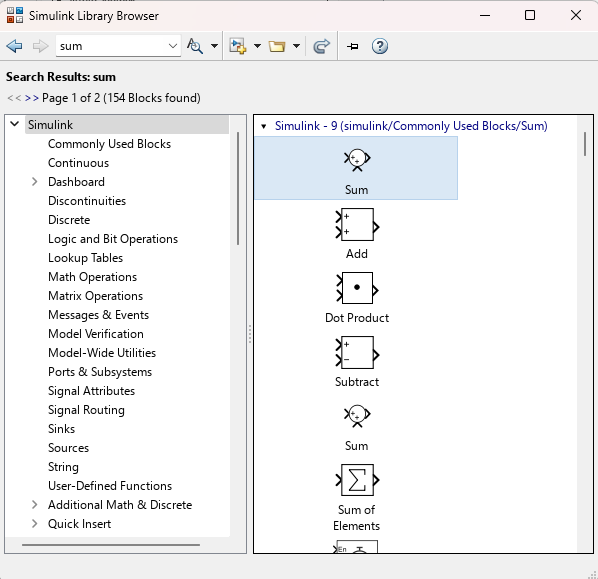
\includegraphics[width=0.45\textwidth]{fig/Capitulo5/Caso_de_estudio_IMU/Generador_de_salidas/libreia_de_bloques_suma.png}
    \caption{Librería de bloques - Suma}
    \label{fig:lib_bloques_add}
\end{figure}

\begin{figure}[h!]
    \centering
    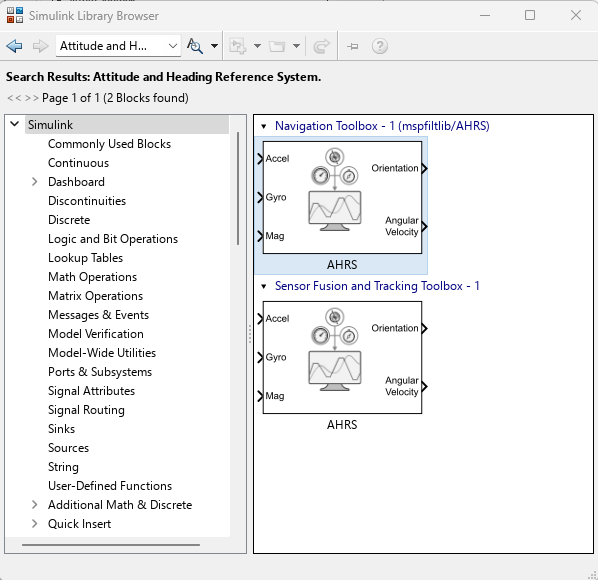
\includegraphics[width=0.45\textwidth]{fig/Capitulo5/Caso_de_estudio_IMU/Generador_de_salidas/libreira_de_bloques_sensor_AHRS.png}
    \caption{Librería de bloques - AHRS}
    \label{fig:lib_bloques_AHRS}
\end{figure}

\begin{figure}[h!]
    \centering
    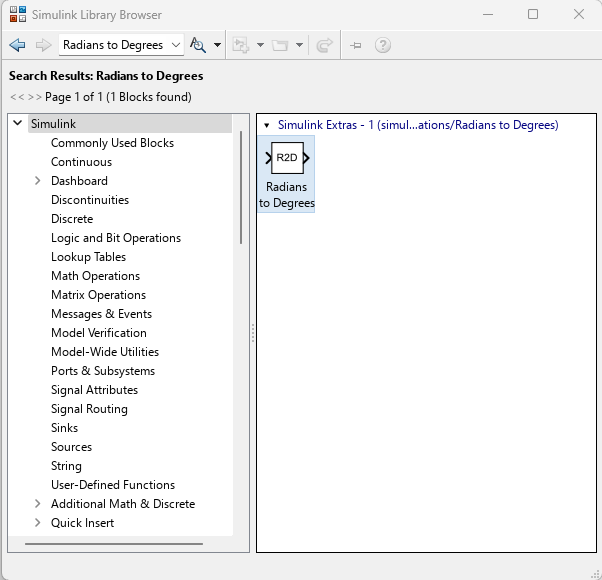
\includegraphics[width=0.45\textwidth]{fig/Capitulo5/Caso_de_estudio_IMU/Generador_de_salidas/libreria_bloque__rad_2_deg.png}
    \caption{Librería de bloques - Conversor de radianes a grados}
    \label{fig:lib_bloques_R2D}
\end{figure}

\begin{figure}[h!]
    \centering
    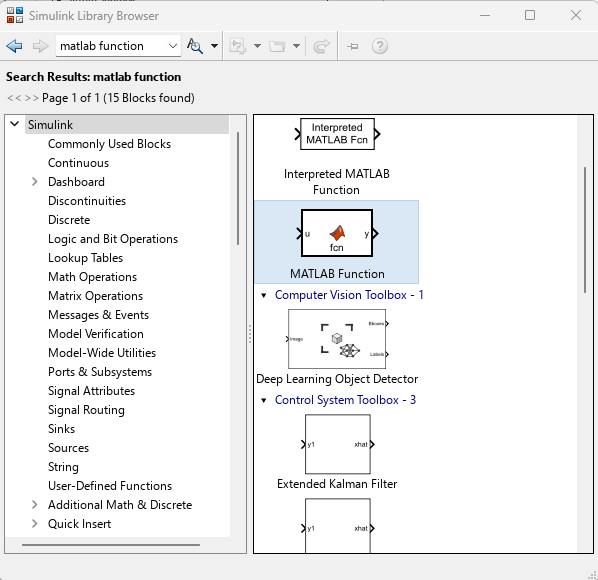
\includegraphics[width=0.45\textwidth]{fig/Capitulo5/Caso_de_estudio_IMU/Generador_de_salidas/libreria_bloque_de_funcion.png}
    \caption{Librería de bloques - Función}
    \label{fig:lib_bloques_func}
\end{figure}

\subsection{Implementación en la Tarjeta de desarrollo mediante EmbedSynthGNC}

\section{Caso de estudio 3 - PID}
\subsection{Implementación en MATLAB Simulink}
\subsection{Implementación en la Tarjeta de desarrollo mediante EmbedSynthGNC}
  \chapter{Conclusiones}

El análisis realizado destacó a la Avnet ZedBoard como una plataforma de desarrollo óptima para el modelado de ingeniería de una computadora de navegación espacial. La arquitectura compartida con la EXA ICEPS, basada en el procesador ARM Cortex-A9 de 32 bits, permitió una comparación detallada y efectiva del rendimiento y las capacidades en un entorno controlado. Esto no solo validó los algoritmos en condiciones seguras, sino que también optimizó significativamente el proceso de desarrollo, preparándolo para su eventual implementación en un sistema crítico. La ZedBoard se consolidó como una herramienta fundamental para avanzar de manera segura y eficiente en el desarrollo de sistemas de guía, navegación y control espacial, cumpliendo satisfactoriamente el objetivo de identificar una plataforma de hardware adecuada para este propósito

Los resultados obtenidos confirman de manera satisfactoria el logro del objetivo propuesto: establecer flujos de trabajo efectivos para el prototipado de algoritmos de control de orientación y navegación con hardware en el loop, específicamente para aplicaciones espaciales. La estrecha concordancia observada entre los resultados de simulación y los datos experimentales, combinada con los bajos porcentajes de error, evidencia la confiabilidad y precisión del marco de trabajo desarrollado. Esta validación asegura que el flujo de trabajo implementado cumple con los requisitos necesarios para la integración y prueba de algoritmos en entornos de hardware en el loop. Por lo tanto, se ha establecido una metodología robusta y fiable para la verificación y validación de sistemas de control de orientación y navegación espacial, lo que será de gran valor en futuras investigaciones y desarrollos en este campo.

La evaluación de los casos de uso de una computadora de navegación y control espacial, a través de la implementación de una aplicación de referencia demostrativa, ha arrojado resultados prometedores. La precisión alcanzada en los modelos de la Unidad de Medición Inercial (IMU) y del controlador PID confirma la capacidad de la aplicación para replicar con exactitud las condiciones reales, lo que es fundamental en entornos de guía, navegación y control espacial.

Los bajos niveles de error registrados en ambos casos demuestran que los modelos implementados no solo capturan fielmente el comportamiento dinámico del sistema, sino que también ofrecen una herramienta confiable para futuras aplicaciones y pruebas. Este alto grado de precisión en la simulación y el control proporciona una base sólida para el uso de esta computadora en misiones donde la precisión y la confiabilidad son críticas.

\chapter{Recomendaciones}

Realizar una evaluación comparativa continua del desempeño de la ZedBoard frente a nuevas plataformas de hardware embebido para mantener actualizado el sistema, considerando nuevas opciones con mayores capacidades o eficiencia energética, especialmente si surgen otros modelos compatibles con ICEPS de EXA.
	
Automatizar el entorno de compilación cruzada mediante scripts y herramientas como CE Docker, para facilitar la generación de binarios para ARM y simplificar la integración de futuros cambios en el código.

Implementar un sistema de versionado y pruebas automatizadas para los archivos de arranque y de sistema. Esto permitirá asegurar la compatibilidad y estabilidad del entorno a lo largo del ciclo de vida del proyecto y en futuras iteraciones.

Diseñar un marco de validación de algoritmos que permita evaluar la efectividad de cada algoritmo de control en simulaciones y pruebas de hardware en lazo cerrado. Esto ayudará a identificar mejoras en su rendimiento y adaptabilidad para aplicaciones GNC complejas

  %----------------------------------------------------------------------------
  % literature in bibtex way:
  % \bibliographystyle{sty/plainurl} % for english documents
  %\bibliography{literatura}
  % literature in biblatex/biber way
  \printbibliography[title={Bibliografía},heading=bibintoc]
  %----------------------------------------------------------------------------

  %----------------------------------------------------------------------------
  \appendix
  %----------------------------------------------------------------------------

  \chapter{Demostración del teorema de Nyquist}
\label{apx:apendice}

El título anterior es solo un ejemplo ilustrativo.  Éste teorema no ameritaría
un apéndice pues es parte normal del currículum de Electrónica, pero apéndices
usualmente involucran aspectos de esta índole, que se salen de la línea de la
tesis, pero que es conveniente incluir por completitud.

Los anexos contienen toda información adicional que se considere pertinente
agregar, como manuales de usuario, demostraciones matemáticas que se salen de
la línea principal de la tesis, pero que pueden considerarse parte de los
resultados del trabajo.


  %----------------------------------------------------------------------------
  \backmatter
  %----------------------------------------------------------------------------

  \printindex                % insert index into document. Don't forget to call
                             % "makeindex filename" first.
\end{document}
